\documentclass[a4paper]{article}
\usepackage{pgf,tikz,pgfplots}
\usetikzlibrary{arrows,decorations.markings}
\pgfplotsset{compat=1.15}
\usepackage{mathrsfs}
\usetikzlibrary{arrows}
\usepackage{array}

\newcolumntype{M}[1]{>{\centering\arraybackslash}m{#1}}
\newcolumntype{N}{@{}m{0pt}@{}}
%% Language and font encodings
\usepackage[english]{babel}
\usepackage[utf8x]{inputenc}
\usepackage[T1]{fontenc}
\usepackage{tensor}
\usepackage{float}
\usepackage[compat=1.1.0]{tikz-feynman}
\tikzfeynmanset{/tikzfeynman/momentum/arrow shorten = 0.3}
\tikzfeynmanset{/tikzfeynman/warn luatex = false}
%% Sets page size and margins
\usepackage[a4paper,top=3cm,bottom=2cm,left=3cm,right=3cm,marginparwidth=1.75cm]{geometry}
\usepackage{fancyhdr}
\pagestyle{fancy}
%% Useful packages
\usepackage{tensor}
\usepackage{xcolor}
\usepackage{color,soul}
\usepackage{amsmath}
\usepackage{amsthm}
\usepackage{enumitem}
\usepackage{eqnarray}
\usepackage{float}
\usepackage{esint}
\usepackage{wrapfig}
\usepackage{gensymb}
\usepackage{lipsum}
\usepackage{amssymb}
\usepackage{array}
\usepackage{tikz}
\usepackage[colorlinks=true, allcolors=blue]{hyperref}
\usepackage{graphicx}
\usepackage{amsmath}
\usepackage{amssymb}
\usepackage{graphicx}
\usepackage[colorlinks=true, allcolors=blue]{hyperref}
\usepackage{mathtools}
\DeclareMathOperator{\Proj}{Proj}
\DeclareMathOperator{\lcm}{lcm}
\DeclareMathOperator{\cosec}{cosec}
\DeclareMathOperator{\sgn}{sgn}
\DeclareMathOperator{\Span}{span}
\DeclareMathOperator{\nullity}{nullity}
\DeclarePairedDelimiter\floor{\lfloor}{\rfloor}
\DeclareMathOperator{\Res}{Res}
\DeclareMathOperator{\rank}{rank}
\DeclareMathOperator{\Ker}{Ker}
\DeclareMathOperator{\R}{R}
\DeclareMathOperator{\Tr}{Tr}
\DeclareMathOperator{\diag}{diag}
\DeclareMathOperator{\Log}{Log}
\DeclareMathOperator{\sech}{sech}
\DeclareMathOperator{\Var}{Var}
\newtheoremstyle{new2}% <name>
{2pt}% <Space above>
{2pt}% <Space below>
{\color{black}}% Body font
{}% <Indent amount>
{\bfseries\color{black}}% Theorem head font
{:}% <Punctuation after theorem head>
{.5em}% <Space after theorem headi>
{}% <Theorem head spec (can be left empty, meaning `normal')>
\theoremstyle{new2}
\newtheorem{ans}{Answer}
\newcommand{\lambdabar}{{\mkern0.75mu\mathchar '26\mkern -9.75mu\lambda}}
\newcommand{\highlight}[1]{%
  \colorbox{red!50}{$\displaystyle#1$}}
  
\definecolor{darkblue}{RGB}{	0, 0, 139}
\newtheoremstyle{new}% <name>
{2pt}% <Space above>
{2pt}% <Space below>
{\color{darkblue}}% Body font
{}% <Indent amount>
{\bfseries\color{black}}% Theorem head font
{:}% <Punctuation after theorem head>
{.5em}% <Space after theorem headi>
{}% <Theorem head spec (can be left empty, meaning `normal')>
\theoremstyle{new}
\newtheorem{qns}{Problem}
\setlength{\parindent}{0cm}
\title{\textbf{Part II PNP Problem Sheet Solutions}}
\author{Tai Yingzhe, Tommy (ytt26)}
\date{}
\setlength{\parindent}{0cm}
\begin{document}
\maketitle
\tableofcontents
\subsection*{Acknowledgements:}
Many thanks to my supervisor JingYuan Shi, and the lecturer Tina Potter for their guidance.
\newpage
\section{Example Sheet 1}
\subsection*{Matter and Forces}
\begin{qns}[Particles]
Explain the meaning of the terms quark, lepton, hadron, nucleus and boson as used in the classification of particles.
\end{qns}
\begin{ans}\leavevmode
\begin{itemize}
    \item Quarks are a type of elementary particle which combine to form composite particles called hadrons. They are the only elementary particles in the Standard Model to experience all four fundamental interactions, and the only known particles with charges being a fraction of the elementary charge.
    \item Leptons are a type of elementary particle with half-integer spin, that does not undergo strong interactions. There are two main classes: charged leptons and neutrinos, with the latter unable to interact with the electromagnetic force.
    \item Hadrons are subatomic composite particles made of two or more quarks held together by the strong force. There are two types: baryons (odd number of quarks) and mesons (even number of quarks). Common examples of baryons are protons and neutrons.
    \item Nucleus is a composite particle made of protons and neutrons.
    \item Bosons are elementary particles with integer spins, and symmetric under exchange. The fundamental forces are mediated by gauge bosons.
\end{itemize}
\end{ans}
\newpage
\subsection*{Relativistic kinematics}
\begin{qns}[Natural units]
Explain what is meant by natural units and the Heaviside-Lorentz system.
\begin{enumerate}[label={(\alph*)}]
\item The reduced Compton wavelength of a particle can be written in natural units as
$$\lambdabar=\frac{1}{m}$$
where $m$ is the mass of the particle. Estimate $\lambdabar$ for a pion ($m_\pi = 139.6$ MeV/c$^2$). Quote your answer in natural units and then convert to SI units.
\item  The total cross-section for $e^+e^-$ annihilation can be written in natural units as
$$\sigma=\frac{4}{3}\frac{\pi\alpha^2}{s}$$
where $\alpha=\frac{1}{137}$ is the fine structure constant and $\sqrt{s}$ is the centre-of-mass energy. Estimate $\sigma$ at a centre-of-mass energy equal to the $Z$ mass ($m_Z = 91.2$ GeV/c$^2$). Calculate your answer in natural units and then convert to barns.
\item  Use dimensional analysis to add the appropriate factors of $\hbar$, $\varepsilon_0$ and $c$ in the formulae for $\lambdabar$ in (a) and for $\sigma$ in (b), and then do the calculations directly in SI units.
\end{enumerate}
Note that $\hbar c=197$ MeV fm, 1 barn $=10^{-28}$ m$^2$.
\end{qns}
\begin{ans}
Natural units is defined by choosing energy as the basic unit (in GeV) and expressing every other quantities in terms of energy.
\begin{itemize}
    \item momentum GeV/c
    \item mass GeV/c$^2$
    \item time (GeV/$\hbar)^{-1}$
    \item length (GeV/$\hbar c)^{-1}$
\end{itemize}
where we can further simplify by setting $\hbar=1=c$.\\[5pt]
Heaviside-Lorentz system: natural units involving electric charge, by further setting $\varepsilon_0,\mu_0$ as 1. In this case, $e=\sqrt{4\pi/137}\sim 0.30$ in natural units.
\begin{enumerate}[label={(\alph*)}]
\item We have $\hbar c=197$ MeV fm, so
$$\lambdabar=\frac{1}{139.6}=7.16\times10^{-3}\text{MeV}^{-1}=1.41~\text{fm}$$
\item We have 1 GeV$^{-1}$ to be 0.197 fm, so 1 GeV$^{-2}$ is $3.89\times10^{-32}$ m$^2$, or 38.9 mb.
$$\sigma=\frac{4}{3}\pi\frac{1}{137^2}\frac{1}{91.2^2}=2.68\times10^{-8}(\text{GeV})^{-2}=0.0104~\text{nb}$$
\item Let $C_1$ and $C_2$ be quantities such that
$$\lambdabar=\frac{C_1}{m},\quad\sigma=\frac{C_2}{s}$$
Since $\lambda=[L]$, $m=[M]$, then $C_1=[L][M]=\hbar/c$. 
$$\lambdabar=\frac{\hbar}{mc}=\frac{6.626\times10^{-34}}{2\pi}\frac{3\times10^8}{139.6\times10^6\times 1.6\times10^{-19}}=1.41\times10^{-15}\text{m}$$
Similarly, $\sigma=[L]^2$ and $s=[M]^2$, then $C_2=[L]^2[M]^2=\hbar^2/c^2$.
$$\sigma=\frac{4}{3}\pi\frac{1}{137^2}\bigg(\frac{6.626\times10^{-34}}{2\pi}\bigg)^2\frac{1}{(91.2\times10^9\times 1.6\times10^{-19})^2}=1.04\times10^{-39}\text{m}^2$$

\end{enumerate}
\end{ans}
\newpage
\begin{qns}[Relativistic kinematics]
Consider the decay of a particle X into two particles a and b.
\begin{enumerate}[label={(\alph*)}]
\item  Show that, in the rest frame of X, the energy of particle a can be written in natural units as
$$E_a=\frac{m_X^2+m_a^2-m_b^2}{2m_X}$$
where $m_i$ is the mass of particle i. What is the equivalent expression for the energy of particle b ? What is the energy if the final state particles are the same (or antiparticles of each other)?
\item  Show that the magnitude of the momentum of particle a can be written in natural units as
$$p_a=\frac{\sqrt{m_X^4+m_a^4+m_b^4-2m_X^2m_a^2-2m_X^2m_b^2-2m_a^2m_b^2}}{2m_X}$$
What is the equivalent expression for the momentum of particle b? What is the value of the momentum if the final state particles are the same (or antiparticles of each other)? Show that if one of the final state particles is massless, e.g. $m_b=0$, then the expression for the momentum simplifies to
$$p_a=\frac{m_X^2-m_a^2}{2m_X}$$
Note: replacing $m_X$ by the centre-of-mass energy, $\sqrt{s}$, in the above gives the equivalent expressions for collision processes.
\item The HERA collider at DESY provided head-on collisions between an electron beam of 27.5 GeV and a proton beam of 920 GeV. What energy of electron beam colliding with a fixed target would be required to obtain the same centre-of-mass energy? Would HERA have had sufficient energy to have produced a Higgs boson of mass 125 GeV?
\end{enumerate}
\end{qns}
\begin{ans}\leavevmode
\begin{enumerate}[label={(\alph*)}]
\item In the rest frame of X, $m_X^2=E_X^2$. By conservation of momentum and energy:
$$\vec{p}_b+\vec{p}_a=0,\quad E_X=E_a+E_b$$
Together with the energy-momentum invariant, these give
$$m_b^2+|\vec{p}_b|^2=E_b^2=(E_X-E_a)^2=E_X^2-2E_XE_a+E_a^2=m_X^2-2m_XE_a+m_a^2+|\vec{p}_a|^2$$
This gives the desired result. Similarly, swap $b\leftrightarrow a$ to get $E_b=\frac{m_X^2+m_b^2-m_a^2}{2m_X}$. If $m_a=m_b$, $E_a=E_b=0.5 m_X$.
\item From the energy-momentum invariant,
$$m_a^2+|\vec{p}_a|^2=E_a^2=\frac{(m_X^2+m_a^2-m_b^2)^2}{(2m_X)^2}$$
Fully expand this to give the desired result. Similarly, by swapping $b\leftrightarrow a$, we obtain $\vec{p}_b$, which we find it to be equal to $\vec{p}_a$ (since expression symmetric in the labels $a,b$). When $m_a=m_b$, then
$$p_a=\frac{\sqrt{m_X^4-4m_X^2m_a^2}}{2m_X}=p_b$$
But, if $m_b=0$, we have
$$p_a=\frac{\sqrt{m_X^4+m_a^4-2m_X^2m_a^2}}{2m_X}=\frac{\sqrt{(m_X^2-m_a^2)^2}}{2m_X}=\frac{m_X^2-m_a^2}{2m_X}$$
\item We are given the energies of the $e^-$ and $p^+$ beams to be 27.5 GeV and 920 GeV respectively. By conservation of momentum and energy:
$$p_p-p_e=p_X,\quad E_e+E_p=E_X$$
By the energy-momentum invariant, $E_X^2-|p_X|^2=m_X^2$. Since $m_e<<E_e$ and $m_p<<E_p$, we have $E_e\approx p_e$ and $E_p\approx p_p$. Hence,
$$E_X=p_e+p_p=E_e+E_p=947.5 GeV,\quad p_X=p_p-p_e=E_p-E_e=892.5~\text{GeV}$$
Using the invariant quantity $s$,
$$s=E_X^2-p_X^2\implies\sqrt{s}=\sqrt{947.5^2-892.5^2}=318~\text{GeV}$$
Now, consider a fixed proton target instead. By conservation of momentum and energy again,
$$p_e=p_p,\quad E_e+E_p=E_X$$
Again, by the energy-momentum invariant, 
$$E_e+m_p=E_X=\sqrt{m_X^2+E_e^2}\implies E_e=\frac{m_X^2-m_p^2}{2m_p}=\frac{318^2-0.938^2}{2(0.938)}=53.9~\text{TeV}$$
where $s=m_X^2$ from earlier. We need a much larger energy if the proton target was fixed.\\[5pt]
Particles of rest mass less than $\sqrt{s}$ can be produced. Since
$$\sqrt{s}=318~\text{GeV}>125~\text{GeV}$$
There is enough energy to create a Higgs boson.
\end{enumerate}
\end{ans}
\begin{qns}[$\Omega$ decay]
The figure shows a photograph and line diagram of the event corresponding to the first observation of the $\Omega^-$ baryon ($\Omega^-\rightarrow\Xi^0\pi^-$, $\Xi^0\rightarrow\Lambda^0\pi^0$) in a K$^-$p interaction in a liquid hydrogen bubble chamber (from Barnes et al., Phys. Rev. Lett. 12 (1964) 204):
\begin{figure}[H]
    \centering
    \includegraphics[scale=0.65]{PS1Q4.JPG}
\end{figure}
\begin{enumerate}[label={(\alph*)}]
\item The two photons from the $\pi^0\rightarrow\gamma\gamma$ decay are both seen to convert to $e^+e^-$ pairs. Show that the process $\gamma\rightarrow e^+e^-$ is kinematically forbidden in vacuo. Explain why the conversion process can take place in the presence of matter, and draw a Feynman diagram representing photon conversion in material, as seen in the figure.
\item The $\pi^-$ and $\Xi^0$ from the $\Omega^-$ decay have momenta of 281 MeV/c and 1906 MeV/c respectively. Their spatial opening angle is 71\degree. Calculate the mass of the $\Omega^-$ and compute its momentum.
\item The length of the $\Omega^-$ flight path is 2.5 cm. Calculate the proper lifetime of the $\Omega^-$.
\end{enumerate}
$m(\pi^-)=139.6$ MeV/c$^2$, $m(\Xi^0)=1315$ MeV/c$^2$.
\end{qns}
\newpage
\begin{ans}\leavevmode
\begin{enumerate}[label={(\alph*)}]
\item Let the 4-momenta be
$$P_\gamma=(E_\gamma,E_\gamma,0,0),\quad P_{e^+}=(E_{e^+},\vec{p}_{e^+}),\quad P_{e^-}=(E_{e^-},\vec{p}_{e^-})$$
By the conservation of energy and momentum:
$$E_\gamma=E_{e^+}+E_{e^-}\implies E_\gamma^2=E_{e^+}^2+E_{e^-}^2+2E_{e^+}E_{e^-}$$
$$E_\gamma=|\vec{p}_{e^+}+\vec{p}_{e^-}|\implies E_\gamma^2=|\vec{p}_{e^+}|^2+|\vec{p}_{e^-}|^2+2\vec{p}_{e^+}\cdot\vec{p}_{e^-}=E_{e^+}^2+E_{e^-}^2-2m_e^2+2|\vec{p}_{e^+}||\vec{p}_{e^-}|\cos\theta$$
These two equations are inconsistent since
\begin{align}
    E_{e^+}E_{e^-}&=\sqrt{|\vec{p}_{e^+}|^2+m_e^2}\sqrt{|\vec{p}_{e^-}|^2+m_e^2}\nonumber\\&=\sqrt{|\vec{p}_{e^+}|^2|\vec{p}_{e^-}|^2+m_e^4+m_e^2(|\vec{p}_{e^+}|^2+|\vec{p}_{e^-}|^2)}\nonumber\\&>|\vec{p}_{e^+}||\vec{p}_{e^-}|\cos\theta-m_e^2\nonumber
\end{align}
In the presence of matter (interactions with particles/nuclei in the medium), there is a term for momentum and energy transferred to the medium. Energy and momentum conservation can now agree. Since one particle is virtual,
\begin{center}
        \begin{tikzpicture}
          \begin{feynman}
            \vertex (i) {$\gamma$};
            \vertex [right=of i] (a);
            \vertex [above right=of a] (f1) {$e^-$};
            \vertex [below right=of a] (f2);
            \vertex [above right=of f2] (f3) {$e^+$};
            \vertex [below =of f2] (f4) {$\gamma$};
            \diagram* {
              (i) -- [photon] (a),
              (f2) --  [edge label=$e^+$] (a) -- (f1),
              (f3) -- (f2) --[photon] (f4)
            };
          \end{feynman}
        \end{tikzpicture}
      \end{center}
\item The reaction is $\Omega^-\rightarrow\Xi^0\pi^-$. The conservation of energy and momentum give
$$E_\Omega=E_\Xi+E_\pi,\quad\vec{p}_\Omega=\vec{p}_\Xi+\vec{p}_\pi$$
The energy-momentum invariant gives
\begin{align}
    m_\Omega^2&=E_\Omega^2-|\vec{p}_\Omega|^2\nonumber\\&=E_\Xi^2+E_\pi^2+2E_\Xi E_\pi-|\vec{p}_\Xi|^2-|\vec{p}_\pi|^2-2|\vec{p}_\Xi||\vec{p}_\pi|\cos\theta\nonumber\\&=m_\Xi^2+m_\pi^2+2E_\Xi E_\pi-2|\vec{p}_\Xi||\vec{p}_\pi|\cos\theta\nonumber
\end{align}
We have $m_\Xi=1315$ MeV/c$^2$, $p_\Xi=1906$ MeV/c and $m_\pi=139.6$ MeV/c$^2$, $p_\pi=281$ MeV/c$^2$. Their energies are then
$$E_\Xi=\sqrt{1315^2+1906^2}=2315.6~MeV,\quad E_\pi=\sqrt{281^2+139.6^2}=313.8~MeV$$
Hence, we have
$$m_\Omega=\sqrt{1315^2+139.6^2+2(2315.6)(313.8)-2(281)(1906)\cos71\degree}=1689 MeV/c^2$$
The momentum is then
$$|p_\Omega|^2=E_\Omega^2-m_\Omega^2=(E_\Xi+E_\pi)^2-m_\Omega^2=(2315.6+313.8)^2-1689^2\implies|p_\Omega|=2015MeV/c$$
\item In the lab frame, the velocity of $\Omega^-$ is 
$$v=\frac{|\vec{p}_\Omega|c}{E_\Omega}=\frac{2015c}{\sqrt{2015^2+1689^2}}=0.766c$$
The measured lifetime in the lab frame is
$$t=\frac{x}{v}=\frac{2.5\times10^{-2}}{0.766\times 3\times10^8}=0.11~\text{ns}$$
where $x$ is the flight path. The proper lifetime (measured in the instantaneous rest frame of $\Omega^-$) is
$$\tau=t/\gamma=0.11\times10^{-9}\sqrt{1-0.766^2}=6.99\times10^{-11}~\text{s}$$
\end{enumerate}
\end{ans}
\subsection*{Decays and reactions}
\begin{qns}[Radioactive decay]
A sample of gold is exposed to a neutron beam of constant intensity such that $10^{10}$ neutrons per second are absorbed in the reaction
$$n+^{197}\text{Au}\rightarrow ~^{198}\text{Au}+\gamma$$
The nuclide $^{198}$Au undergoes $\beta$ decay to $^{198}$Hg with a mean lifetime of 4 days.
\begin{enumerate}[label={(\alph*)}]
\item How many atoms of $^{198}$Au will be present after 6 days of irradiation?
\item How many atoms of $^{198}$Hg will be present after 6 days assuming that the neutron beam has no effect on the Hg?
\item  What is the equilibrium number of $^{198}$Au nuclei?
\end{enumerate}
\end{qns}
\begin{ans}\leavevmode
\begin{enumerate}[label={(\alph*)}]
\item Let the number of $^{198}$ Au atoms be $N_2$, then it satisfies a differential equation
$$\frac{dN_2}{dt}=\lambda_1N_1-\lambda_2N_2$$
where $\lambda_1N_1$ is the number of neutrons per unit time ($\lambda_1N_1=10^{10}$ s$^{-1}$) and $\lambda_2$ is the inverse of its lifetime $\lambda_2=\frac{1}{\tau}$ which is 0.25 day$^{-1}$. Assuming the irridation starts at $t=0$, then
\begin{align}
    T=\int_0^Tdt&=\frac{1}{\lambda_1N_1}\int_0^{N(T)}\frac{1}{1-\frac{\lambda_2}{\lambda_1}\frac{N_2}{N_1}}dN_2\nonumber\\&=\frac{1}{\lambda_1N_1}\frac{-\lambda_1N_1}{\lambda_2}\ln\bigg|1-\frac{\lambda_2N}{\lambda_1N_1}\bigg|\nonumber\\&=\frac{1}{\lambda_2}\ln\frac{\lambda_1N_1}{\lambda_1N_1-\lambda_2N}\implies N(T)=\frac{\lambda_1N_1}{\lambda_2e^{\lambda_2T}}(e^{\lambda_2T}-1)\nonumber
\end{align}
Let $T=6$ days, then $N=2.68\times10^{15}$ (convert days to SI units).
\item Let $N_3$ be the number of $^{198}$Hg, then
\begin{align}
    \frac{dN_3}{dt}&=\lambda_2N_2(t)=\lambda_1N_1(1-e^{-\lambda_2t})\nonumber\\
    N_3&=\lambda_1N_1\bigg(T+\frac{1}{\lambda_2}e^{-\lambda_2T}-\frac{1}{\lambda_2}\bigg)=10^{10}(6+4e^{-6/4}-4)=2.50\times10^{15}\nonumber
\end{align}
\item At equilibrium, $\frac{dN_2}{dt}=0$, so
$$\lambda_1N_1=\lambda_2N_{\text{eq}}\implies N_{\text{eq}}=\frac{\lambda_1N_1}{\lambda_2}=\lambda_1N_1\tau_2=10^{10}\times 4\times 24\times 3600=3.46\times10^{15}$$
\end{enumerate}
\end{ans}
\newpage
\begin{qns}[Caesium decay]
The decay chain $^{139}$Cs$\rightarrow$ $^{139}$Ba $\rightarrow$ $^{139}$La is observed for an initially pure sample of 1mCi of $^{139}$Cs. The half life of $^{139}$Cs is 9.5 minutes and that of $^{139}$Ba is 82.9 minutes; $^{139}$La is stable. Write down the rate equations for this system, and show that the number of Ba atoms present at time $t$ is given by
$$N_{\text{Ba}}(t)=\frac{\lambda_{\text{Cs}}N_{\text{Cs}}(0)}{\lambda_{\text{Ba}}-\lambda_{\text{Cs}}}[e^{-\lambda_{\text{Cs}}t}-e^{-\lambda_{\text{Ba}}t}]$$
in an obvious notation, where the $\lambda$ values represent the corresponding decay rates. What is the maximium $^{139}$Ba activity (i.e. rate of $^{139}$Ba decay), and at what time does it occur?\\[5pt]
1 Ci $=3.7\times10^{10}$ disintegrations per second.
\end{qns}
\begin{ans}
The coupled first order differential equations are
$$\frac{dN_{\text{Cs}}}{dt}=-\lambda_{\text{Cs}}N_{\text{Cs}},\quad\frac{dN_{\text{Ba}}}{dt}=\lambda_{\text{Cs}}N_{\text{Cs}}-\lambda_{\text{Ba}}N_{\text{Ba}},\quad\frac{dN_{\text{La}}}{dt}=\lambda_{\text{Ba}}N_{\text{Ba}}$$
The first gives $N_{\text{Cs}}=N_{\text{Cs},0}e^{-\lambda_{\text{Cs}}t}$, and the second can thus be solved by an integration factor:
\begin{align}
    \frac{dN_\text{Ba}}{dt}+\lambda_{\text{Ba}}N_{\text{Ba}}&=\lambda_{\text{Cs}}N_{\text{Cs},0}e^{-\lambda_{\text{Cs}}t}\nonumber\\e^{\lambda_{\text{Ba}}t}N_{\text{Ba}}&=\lambda_{\text{Cs}}N_{\text{Cs},0}\int_0^te^{(\lambda_{\text{Ba}}-\lambda_{\text{Cs}})t}dt\nonumber\\N_{\text{Ba}}&=\frac{\lambda_{\text{Cs}}N_{\text{Cs},0}e^{-\lambda_{\text{Ba}}t}}{\lambda_{\text{Ba}}-\lambda_{\text{Cs}}}[e^{(\lambda_{\text{Ba}}-\lambda_{\text{Cs}})t}-1]\nonumber\\&=\frac{\lambda_{\text{Cs}}N_{\text{Cs},0}}{\lambda_{\text{Ba}}-\lambda_{\text{Cs}}}(e^{-\lambda_{\text{Cs}}t}-e^{-\lambda_{\text{Ba}}t})\nonumber
\end{align}
The activity $\lambda_{\text{Ba}}N_{\text{Ba}}$ is maximum when $\frac{dN_{\text{Ba}}}{dt}=0$, i.e.
\begin{align}
    \lambda_{\text{Cs}}N_{\text{Cs},0}e^{-\lambda_{\text{Cs}}t}&=\frac{\lambda_{\text{Ba}}\lambda_{\text{Cs}}N_{\text{Cs},0}}{\lambda_{\text{Ba}}-\lambda_{\text{Cs}}}(e^{-\lambda_{\text{Cs}}t}-e^{-\lambda_{\text{Ba}}t})\nonumber\\\implies\frac{\lambda_{\text{Ba}}}{\lambda_{\text{Cs}}}&=e^{-(\lambda_\text{Cs}-\lambda_{\text{Ba}})t}\nonumber\\\implies t&=\frac{1}{\tau_{\text{Cs}}^{-1}-\tau_{\text{Ba}}^{-1}}\ln\frac{\tau_{\text{Ba}}}{\tau_{\text{Cs}}}=\frac{\ln(82.9/9.5)}{\ln2(9.5^{-1}-82.9^{-1})}=\frac{23.2}{\ln 2}=33.5 min\nonumber
\end{align}
The corresponding maximum activity is
$$\lambda_\text{Cs}N_{\text{Cs}}e^{-\lambda_{\text{Cs}}(33.5)}=0.087mCi$$
\end{ans}
\newpage
\begin{qns}[Kaon decay]\leavevmode
\begin{enumerate}[label={(\alph*)}]
\item  Calculate the branching fraction for the decay $K^+\rightarrow\pi^+\pi^0$, given that the partial width for this decay is 1.2 $\times10^{-8}$ eV and the mean lifetime of the K$^+$ meson is 1.2 $\times10^{-8}$ s.
\item A beam of K$^+$ mesons of momentum 10 GeV is produced. What fraction of them will remain undecayed 100 m downstream?
\item When the K$^+$ mesons decay to $\pi^+\pi^0$, what are the minimum and maximum laboratory energies of the produced $\pi^+$ mesons?
\end{enumerate}
\end{qns}
\begin{ans}\leavevmode
\begin{enumerate}[label={(\alph*)}]
\item The branching fraction is
$$B_f=\frac{\Gamma_f}{\Gamma}=\Gamma_f\tau=(1.2\times10^{-8})(1.82\times10^7)=0.218$$
where we converted $\tau$ to $1/eV$ units via 1s$=\hbar^{-1}=1.515\times10^{15}$ (eV)$^{-1}$.
\item The fraction decayed will be
$$e^{-t/\tau}=e^{-x/v\gamma\tau_0}=\exp\bigg(-\frac{x}{\tau_0}\frac{m_{K^+}}{E_{K^+}}\frac{E_{K^+}}{p_{K^+}c}\bigg)=\exp\bigg(-\frac{100}{1.2\times10^{-8}}\frac{0.4937}{10(3\times10^8)}\bigg)=0.254$$
\item In the rest frame of $K^+$, we have
$$E_{\pi^+}=\frac{m_{K^+}^2+m_{\pi^+}^2-m_{\pi^0}^2}{2m_{K^+}}=248.1 MeV:=E_0$$
$$p_{\pi^+}=\frac{\sqrt{m_{K^+}^4+m_{\pi^+}^4+m_{\pi^0}^4-2m_K^2+m_\pi^2-2m_K^2+m_{\pi^0}^2-2m_{\pi^+}^2 m_{\pi^0}^2}}{2m_{K^+}}=205.1MeV:=p_0$$
where we used the results from Q3, and $m_{\pi^+}=139.6$ MeV/c$^2$, $m_{\pi^0}=134.98$ MeV/c$^2$, $m_{K^+}=493.7$ MeV. The minimum and maximum laboratory energies are
$$E_{\text{lab}}=\gamma(E_0\pm\beta p_0)$$
which gives a maximum of 9200 MeV and 877 MeV, where we have
$$\gamma=\frac{E_{K^+}}{m_{K^+}}=\frac{\sqrt{0.4937^2+10^2}}{0.4937}=20.3,\quad\beta=\frac{p_{K^+}}{E_{K^+}}=\frac{10}{\sqrt{0.4937^2+10^2}}=0.999$$
\end{enumerate}
\end{ans}
\newpage
\begin{qns}[Cross-sections]
Define the terms total cross-section and differential cross-section for scattering processes.\\[5pt]
A beam of neutrons with an intensity $10^5$ particles per second traverses a thin foil of $^{235}$U with a ”thickness” of $10^{−1}$ kg m$^{−2}$.\\[5pt]
There are three possible outcomes when a neutron interacts with a $^{235}$U nucleus:
\begin{enumerate}[label={(\roman*)}]
    \item elastic scattering of the neutron, with a cross-section $10^{−2}$ b ;
    \item the capture of the neutron followed by the emission of a $\gamma$-ray., with cross-section 70 b;
    \item the capture of the neutron, followed by the resulting nucleus undergoing fission with cross-section 200 b.
\end{enumerate}
Using this information, determine
\begin{enumerate}[label={(\alph*)}]
\item the intensity of the neutron beam transmitted by the foil;
\item  the rate of fission reactions occurring in the foil induced by the incident beam;
\item the flux of neutrons elastically scattered out of the beam at a point 10 m from the foil, assuming that the neutrons are scattered isotropically.
\end{enumerate}
\end{qns}
\begin{ans}
The total cross-section is the reaction rate per target particle per unit incident flux ($\sigma=\Gamma/\Phi$) over all directions. On the other hand, the differential cross-section is the number of particles scattered per unit time and per unit solid angle (either in real space or momentum space), per unit incident flux, per target particle.
\begin{enumerate}[label={(\alph*)}]
\item The number of neutrons scattered per unit time is
$$N=N_{\text{beam}}\sigma ndx=10^5(70+200+0.01)\times10^{-28}\frac{10^{-1}}{235(1.66\times10^{-27})}=692~\text{s}^{-1}$$
where we summed over the scattering cross-sections for all the scattering processes (i)-(iii). The total number transmitted is
$$N=10^5-692=99308s^{-1}$$
\item The fission rate is
$$\frac{\sigma_{\text{fission}}}{\sigma_{\text{total}}}\Gamma=\frac{200}{270.01}692=512~\text{s}^{-1}$$
\item The scattering rate is
$$\frac{\sigma_{\text{rate}}}{\sigma_{\text{total}}}\Gamma=\frac{0.01}{270.01}692=0.0256~\text{s}^{-1}$$
The flux at $r=10$ m is
$$\Phi=\frac{0.0256}{4\pi(10)^2}=2.04\times10^{-5}~\text{m}^{-2}~\text{s}^{-1}$$
\end{enumerate}
\end{ans}
\newpage
\begin{qns}[Breit-Wigner formula]
The Breit-Wigner formula for a reaction cross-section is given by
$$\sigma(E)=\frac{\pi g}{p_i^2}\frac{\Gamma_i\Gamma_f}{(E-E_0)^2+\Gamma^2/4}$$
Explain the meaning of the symbols in this equation, and outline its derivation.\\[5pt]
The maximum value of the cross-section for radiative capture of neutrons in $^{123}$Te (i.e. the process $n +~^{123}$ Te $\rightarrow$ $^{124}$ Te $+\gamma$) is 75 kb and is reached at a neutron energy of 2.2 eV, where the elastic width $\Gamma_n$ is 0.0104 eV and the radiative width $\Gamma_\gamma$ is 0.105 eV. The spin of $^{123}$Te in its ground state is $J=1/2$. What is the elastic cross-section at resonance and what is the spin of the compound nucleus formed?
\end{qns}
\begin{ans}\leavevmode
\begin{itemize}
    \item $\sigma(E)$ gives the cross-section of a reaction, usually involving an intermediate resonant state
    \item $g$ is the ratio of number of spin states for the resonant state to the total number of initial spin states
    \item $p_i$ is the initial momentum, in the centre-of-mass frame
    \item $\Gamma_i$ and $\Gamma_f$ are partial decay rates for the reactions `initial state'$\rightarrow Z^*$ and $Z^*\rightarrow$ `final state' respectively
    \item $E_0$ is the mass of the resonant state
    \item $E$ is the total energy
    \item $\Gamma$ is the total decay rate, which is also $1/\tau$ (inverse of the lifetime of the resonant state).
\end{itemize}
To derive the Breit-Wigner formula, we start from $\sigma=\frac{\Gamma}{\Phi}$, where the flux is $\Phi=\frac{v_iAn}{A}=v_in$ ($v_i$ is the velocity of the incoming beam, and $n$ is the number density of incident particles) and $\Gamma$ is obtained from Fermi's Golden rule:
$$\Gamma=2\pi|\mathcal{M}_{fi}|^2\rho(E_f)=2\pi|\mathcal{M}_{fi}|^2\frac{p_f^2}{(2\pi)^3v_f}\int d\Omega=\frac{|\mathcal{M}_{fi}|^2p_f^2}{\pi v_f}$$
where $\rho(E_f)$ is the density of states at energy $E_f$. To compute the density of states, consider periodic boundary conditions, then
$$dN=\bigg(\frac{L}{2\pi}\bigg)^3p^2dpd\Omega\rightarrow\rho(p)=\frac{dN}{dp}=\bigg(\frac{L}{2\pi}\bigg)^3p^2d\Omega\implies\rho(E)=\frac{dN}{dp}\frac{dp}{dE}=\bigg(\frac{L}{2\pi}\bigg)^3\frac{p^2}{v}d\Omega$$
The $L^3$ factor cancels off from the normalization factor of $|\mathcal{M}_{fi}|^2$. The matrix element $\mathcal{M}_{fi}$ is computed from second-order perturbation theory, i.e. 
$$\mathcal{M}_{fi}=\sum_Z\frac{M_{iZ}M_{Zf}}{E-E_Z}$$
where we sum over all intermediate states. Close to a particular $E_Z$, only one intermediate state dominates. Let this state be $\psi(t)=\psi(0)\exp(-i(E_0-i0.5\Gamma)t)$ with $E_Z=E_0-i0.5\Gamma$. Hence,
$$|\mathcal{M}_{fi}|^2=\frac{|\mathcal{M}_{iZ}|^2|\mathcal{M}_{Zf}|^2}{(E-E_0)^2+0.25\Gamma^2}$$
where the individual matrix elements satisfy the Fermi's Golden rule, i.e. $\Gamma_{Z\rightarrow f}=\frac{|\mathcal{M}_{Zf}|^2p_f^2}{\pi v_f}$ and $\Gamma_{i\rightarrow Z}=\frac{|\mathcal{M}_{iZ}|^2p_i^2}{\pi v_i}$. Putting them altogether, the total cross-section is
\begin{align}
\sigma&=\frac{1}{v_i}\frac{p_f^2}{\pi v_f}\frac{|\mathcal{M}_{iZ}|^2|\mathcal{M}_{Zf}|^2}{(E-E_0)^2+\Gamma^2/4}\nonumber\\&=\frac{1}{v_i}\frac{p_f^2}{\pi v_f}\Gamma_{i\rightarrow Z}\frac{\pi v_i}{p_i^2}\Gamma_{Z\rightarrow f}\frac{\pi v_f}{p_f^2}\frac{1}{(E-E_0)^2+0.25\Gamma^2}\nonumber\\&=\frac{\pi}{p_i^2}\frac{\Gamma_{Z\rightarrow f}\Gamma_{i\rightarrow Z}}{(E-E_0)^2+0.25\Gamma^2}\nonumber
\end{align}
where the factor $L^3$ in $\Phi=v_i/L^3$ (there is one particle per $L^3$ volume) is again cancelled out by the normalization factor of the transition matrix element. Finally, we add the factor $g$ to account for spin:
$$g=\frac{2J_Z+1}{(2J_a+1)(2J_b+1)}$$
This was necessary, since this is the probability for the initial particles a and b, to collide to the correct spin state to form Z.\\[5pt]
For the problem on hand, we have two possible collisions:
\begin{itemize}
    \item an elastic one involving only $n$ and $^{123}$Te;
    \item an inelastic one, which involves an emission of a photon.
\end{itemize}
We are given the partial widths, and can be used to find the partial cross-sections:
$$\frac{\sigma_n}{\sigma_\gamma}=\frac{\pi g\Gamma_n^2}{p_n^2\Gamma^2/4}\frac{p_n^2\Gamma^2/4}{\pi g\Gamma_n\Gamma_\gamma}=\frac{\Gamma_n}{\Gamma_\gamma}\implies\sigma_n=75\times10^3\frac{0.0104}{0.105}=7.4\times10^3b$$
Since the neutron has energy of 2.2 eV, it is non-relativistic, and we may approximate its momentum classically:
$$p_n=\sqrt{2mE_n}=\sqrt{2(939\times10^6)(2.2)}=6.43\times10^4eV=3.25\times10^{11}m^{-1}$$
where we used 
$$c\hbar=1.978\times10^{-7}eV~m=1\implies 1eV=5.054\times10^6m^{-1}$$
to convert $p$ to a length scale. We can thus find $g$ from $\sigma_n$:
$$g=\frac{\sigma_np_n^2}{4\pi}\frac{\Gamma^2}{\Gamma_n^2}=\frac{(7.43\times10^{-25})(3.25\times10^{11})^2}{4\pi}\bigg(\frac{0.0104+0.105}{0.0104}\bigg)^2=0.7689\approx 0.5$$
Since the spin of $^{123}Te$ in the ground state and that of the neutron is $1/2$, we must have
$$g=\frac{2J_Z+1}{(2(0.5)+1)(2(0.5)+1)}=0.75\implies J_Z=1$$
The compound nucleus is a boson.
\end{ans}
\newpage
\section{Example Sheet 2}
\subsection*{Colliders and detectors}
\begin{qns}[Detector Signatures]
For each $e^+e^-$ process below, sketch the signature in a typical cylindrical detector
\begin{figure}[H]
    \centering
    \includegraphics[scale=0.4]{detectorQ.JPG}
\end{figure}
\begin{enumerate}[label=(\alph*)]
    \item $e^+e^-\rightarrow\mu^+\mu^-e^+e^-$
    \item $e^+e^-\rightarrow\mu^+\mu^-\gamma$
    \item $e^+e^-\rightarrow\nu\overline{\nu}\gamma$
    \item $e^+e^-\rightarrow\tau^+\tau^-$ where the taus decay as $\tau^-\rightarrow e^-\overline{\nu}_e\nu_\tau$ and $\tau^+\rightarrow\pi^+\pi^0\overline{\nu}_\tau$.
    \item $e^+e^-\rightarrow\pi^+n\overline{p}\pi^0K^+K^-$
\end{enumerate}
Draw the lowest order Feynman diagram for (a)-(d).
\end{qns}
\begin{ans}\leavevmode
\begin{enumerate}[label=(\alph*)]
\item The electron and positron will show up as tracks (curvature of track consistent with the sign of the charged particle) in the tracker, with energy deposits in the electron calorimeter. The muons are more penetrating and will go further, and thus be detected in the muon spectrometer.
\begin{figure}[H]
    \centering
    \includegraphics[scale=0.4]{detectora.JPG}
\end{figure}
In drawing the Feynman diagram, remember to conserve lepton number and charge.
\begin{center}
    \begin{tikzpicture}
      \begin{feynman}
        \vertex (m1);
        \vertex [left=0.7em of m1] {$Qe$};
        \vertex [above left=of m1] (i1) {$e^-$};
        \vertex [below left=of m1] (i2) {$e^+$};
        \vertex [right=of m1] (m2);
        \vertex [right=0.7em of m2] {$Qe$};
        \vertex [right= of f2] (m3);
        \vertex [right=0.7em of m3] {$Qe$};
        \vertex [above right=of m2] (f2) {$e^+$};
        \vertex [below right=of m2] (f1);
        \vertex [above right=of m3] (f5) {$\mu^+$};
        \vertex [below right=of m3] (f4) {$\mu^-$};
         \vertex [below right =of f1] (f6);
         \vertex [left=0.7em of f1] {$Qe$};

        \diagram*{
          (i1) -- [fermion] (m1) -- [fermion] (i2),
          (f2) -- [fermion] (m2) -- [fermion, edge label=$e^-$] (f1),
          (m1) -- [photon, edge label=$\gamma$] (m2),
          (f1) -- [photon, edge label=$\gamma$] (m3) -- [fermion] (f4),
          (f1) --[fermion] (f6),
          (f5) -- [fermion] (m3) 
        };
      \end{feynman}
    \end{tikzpicture}
\end{center}
\item The muon and anti-muon will show up as tracks (curvature of track consistent with the sign of the charged particle) in the tracker, with energy deposits in the electron calorimeter. They penetrate through and will be detected in the muon spectrometer. The photons (being neutral) do not leave any tracks behind, but only energy deposits.
\begin{figure}[H]
    \centering
    \includegraphics[scale=0.4]{detectorb.JPG}
\end{figure}
In drawing the Feynman diagram, remember to conserve lepton number and charge.
\begin{center}
    \begin{tikzpicture}
      \begin{feynman}
        \vertex (m1);
        \vertex [left=0.7em of m1] {$e$};
        \vertex [above left=of m1] (i1) {$e^-$};
        \vertex [below left=of m1] (i2) {$e^+$};
        \vertex [right=of m1] (m2);
        \vertex [right=0.7em of m2] {$e$};
        \vertex [right= of f1] (m3);
        \vertex [above right=of m2] (f1) {$\mu^-$};
        \vertex [below right=of m2] (f2);
         \vertex [below right =of f2] (f6);
        \vertex [left=0.7em of f2] {$e$};

        \diagram*{
          (i1) -- [fermion] (m1) -- [fermion] (i2),
          (m2) -- [fermion] (f1),
          (f2)-- [fermion, edge label=$\mu^+$] (m2),
          (m1) -- [photon, edge label=$\gamma$] (m2),
          (f6) --[fermion] (f2),
          (f2) -- [photon, edge label=$\gamma$] (m3)
        };
      \end{feynman}
    \end{tikzpicture}
\end{center}
\item The neutrinos will not be detected in this setup. The photons (being neutral) do not leave any tracks behind, but only energy deposits.
\begin{figure}[H]
    \centering
    \includegraphics[scale=0.4]{detectorc.JPG}
\end{figure}
In drawing the Feynman diagram, remember to conserve lepton number and charge. Since neutrinos are involved, we require W gauge bosons which are mediator of the weak interaction.
\begin{center}
        \begin{tikzpicture}
          \begin{feynman}
            \vertex (i) {$e^-$};
            \vertex [right=of i] (a);
            \vertex [right=0.7em of a] {$g_W$};
            \vertex [above right=of a] (f1) {$\nu_e$};
            \vertex [below right=of a] (f2);
            \vertex [left=0.7em of f2] {$e$};
            \vertex [right=of f2] (f3) {$\gamma$};
            \vertex [below left =of f2] (f4);
            \vertex [below =0.7em of f4] {$g_W$};
            \vertex [below right =of f4] (f5){$\overline{\nu}_e$};
            \vertex [left =of f4] (f6) {$e^+$};
            \diagram* {
              (i) -- [fermion] (a)--[fermion] (f1),
              (f2) --  [photon, edge label=$W^-$] (a) -- (f1),
              (f3) -- [photon] (f2) --[photon, edge label=$W^+$] (f4),
              (f4) -- [fermion] (f6),
              (f5)--[fermion] (f4),
            };
          \end{feynman}
        \end{tikzpicture}
      \end{center}
\item $\pi^+$ and $\pi^0$ are hadrons (and will thus form deposits in the hadron calorimeter), and consists of quarks, so strong interactions are involved. Again, neutrinos are not detected in this setup. Since $\pi^+$ and $e^0$ are charged particles, they will form tracks, with curvatures consistent with their charge sign, in the tracker. The electron will form energy deposits in the electron calorimeter.
\begin{figure}[H]
    \centering
    \includegraphics[scale=0.4]{detectord.JPG}
\end{figure}
In drawing the Feynman diagram, remember to conserve lepton number and charge. Since neutrinos are involved, we require W gauge bosons which are mediator of the weak interaction. Let the pions have composition $\pi^+$ (u$\overline{d}$) and $\pi^0$ (u$\overline{u}$).
\begin{center}
    \begin{tikzpicture}
      \begin{feynman}
        \vertex (m1);
        \vertex [left=0.7em of m1] {$e$};
        \vertex [above left=of m1] (i1) {$e^-$};
        \vertex [below left=of m1] (i2) {$e^+$};
        \vertex [right=of m1] (m2);
        \vertex [below = 0.7em of m2] {$e$};
        
        
        \vertex [right= of f2] (m3);
        \vertex [left=0.7em of f2] {$g_W$};
        \vertex [right=0.7em of m3] {$g_W$};
        \vertex [above right=of m2] (f2);
        \vertex [below right=of m2] (f1);
         \vertex [below right =of f1] (f6){$\nu_\tau$};
         \vertex [above right=of m3] (f4) {$e^-$};
        \vertex [below right=of m3] (f5){$\overline{\nu}_e$};
        
        \vertex [above right=of f2] (f7);
        \vertex [right=0.7em of f7] {$g_W$};
        \vertex [below right=of f2] (f8) {$\overline{\nu}_\tau$};
        \vertex [above right=of f7] (f9);
        \vertex [left=0.7em of f9] {$\sqrt{\alpha_s}$};
        \vertex [above right =of f9](f13){$u$};
        
        \vertex [below right=of f7] (f10){$\overline{d}$};
        \vertex [right=of f9] (m4);
        \vertex [right=0.7em of m4] {$\sqrt{\alpha_s}$};
        \vertex [above right=of m4] (f11){$\overline{u}$};
        \vertex [below right=of m4] (f12){$u$};

        \diagram*{
          (i1) -- [fermion] (m1) -- [fermion] (i2),
          (f2) -- [fermion, edge label=$\tau^+$] (m2),
          (m2)-- [fermion, edge label=$\tau^-$] (f1),
          (m1) -- [photon, edge label=$\gamma/Z$] (m2),
          (f1) --[fermion] (f6),
          (f1) -- [photon, edge label=$W^-$] (m3),
          (m3) -- [fermion] (f4),
          (f5) -- [fermion] (m3),
          (f8) -- [fermion] (f2),
          (f2) -- [photon, edge label=$W^+$] (f7),
          (f7) --[fermion, edge label=$u$] (f9),
          (f10) --[fermion] (f7),
          (f9) -- [gluon] (m4),
          (f11) --[fermion] (m4),
          (m4) -- [fermion] (f12),
          (f9) -- [fermion] (f13)
        };
      \end{feynman}
    \end{tikzpicture}
\end{center}
where the taus decay as $\tau^-\rightarrow e^-\overline{\nu}_e\nu_\tau$ and $\tau^+\rightarrow\pi^+\pi^0\overline{\nu}_\tau$. The pions $\pi^+$ and $\pi^0$ are $u\overline{d}$ and $u\overline{u}$ respectively.
\item The charged particles will all produce tracks, with curvature consistent with their signs, as well as, energy deposits in the electron calorimeter. The hadrons ($\overline{p}$, $n$, $K^\pm$, $\pi^{0,+}$) will form energy deposits in the hadronic calorimeter. 
\begin{figure}[H]
    \centering
    \includegraphics[scale=0.5]{detectore.JPG}
\end{figure}
\end{enumerate}
\end{ans}
\newpage
\begin{qns}[Detector Resolution]\leavevmode
\begin{enumerate}[label=(\alph*)]
\item In an experiment, the momentum measurement accuracy of the tracking detector is 1\% for 1 GeV muons. What is the momentum accuracy for 20 GeV muons in the same apparatus?
\item The energy resolution for 1 GeV electrons in the electromagnetic calorimeter is 0.5\%. What is the energy resolution for 10 GeV electrons?
\end{enumerate}
\end{qns}
\begin{ans}
Let the measurement accuracy/resolution be $\sigma$, $p$ be momentum and $E$ be energy.
\begin{enumerate}[label=(\alph*)]
\item The momentum accuracy $\sigma_p/p\propto p$ is $\frac{\sigma_p}{p}=1\%\times \frac{20}{1}=0.2$.
\item The energy resolution $\sigma_E/E\propto1/\sqrt{E}$ is $\frac{\sigma_E}{E}=0.5\%\times\sqrt{\frac{1}{10}}=0.00158$.
\end{enumerate}
\end{ans}
\subsection*{Feynman diagrams and QED}
\begin{qns}[QED Feynman Diagrams]
Draw the lowest order Feynman diagram(s) for each of the following processes:
\begin{enumerate}[label=(\alph*)]
\item $\gamma\rightarrow e^+e^-$ (in matter)
\item $e^-e^-\rightarrow e^-e^-$
\item $e^+e^-\rightarrow e^+e^-$
\item $e^+e^-\rightarrow \mu^+\mu^-$
\item $e^+e^-\rightarrow \gamma\gamma$
\item $\gamma\gamma\rightarrow\gamma\gamma$
\end{enumerate}
\end{qns}
\begin{ans}\leavevmode
\begin{enumerate}[label=(\alph*)]
\item t-channel: the vertical propagator is the sum of two time-ordering, which includes the case of a virtual positron moving backwards in time (arrow still directed upward) and a virtual electron moving forward in time (arrow still directed upward).
\begin{center}
    \begin{tikzpicture}
      \begin{feynman}
        \vertex (m1);
        \vertex [above=0.7 em of m1] {$e$};
        \vertex [above left= of m1](i1) {$\gamma$};
        \vertex [above right= of m1](f1){$e^-$};
        \vertex [below= of m1](m2);
        \vertex [left=0.7 em of m2] {$e$};
        \vertex [right= of m2](f2){$e^+$};
        \vertex [below= of m2](m3);
         \vertex [below left=of m3] (i2) {$Ze$};
        \vertex [below right=of m3] (f3) {$Ze$};
        \diagram*{
          (i1) -- [photon] (m1) -- [fermion] (f1),
          (m2) -- [fermion, edge label=$e^\pm$] (m1),
          (f2) -- [fermion] (m2),
          (m2) -- [photon] (m3),
          (i2) -- [fermion] (m3),
          (m3) -- [fermion] (f3)
        };
      \end{feynman}
    \end{tikzpicture}
\end{center}
\item Identical particles are involved in the final state, so both `t-channel' and `u-channel' are allowed. We cannot have the `s-channel' since charge will not be conserved at the vertices. Draw the `t-channel':
\begin{center}
    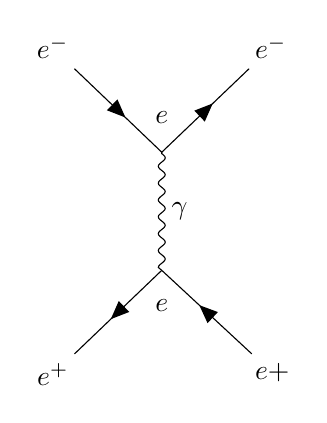
\begin{tikzpicture}
      \begin{feynman}
        \vertex (m1);
        \vertex [above=0.7 em of m1] {$e$};
        \vertex [above left= of m1](i1) {$e^-$};
        \vertex [above right= of m1](f1){$e^-$};
        \vertex [below= of m1](m2);
        \vertex [below=0.7 em of m2] {$e$};
        \vertex [below right= of m2](f2){$e+$};
        \vertex [below left= of m2](i2){$e^+$};
        \diagram*{
          (i1) -- [fermion] (m1) -- [fermion] (f1),
          (m1) -- [photon, edge label=$\gamma$] (m2),
          (m2) -- [fermion] (i2),
          (f2) -- [fermion] (m2)
        };
      \end{feynman}
    \end{tikzpicture}
\end{center}
\item Annihilation process, so draw `s-channel'. Could also have `t-channel' (electron scatters off positron).
\begin{center}
    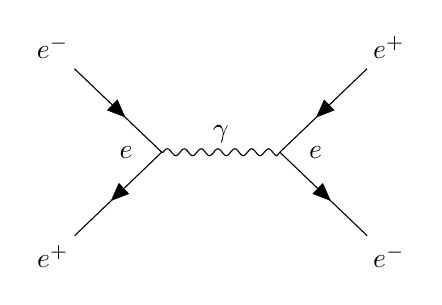
\begin{tikzpicture}
      \begin{feynman}
        \vertex (m1);
        \vertex [left=0.7em of m1] {$e$};
        \vertex [above left=of m1] (i1) {$e^-$};
        \vertex [below left=of m1] (i2) {$e^+$};
        \vertex [right=of m1] (m2);
        \vertex [right=0.7em of m2] {$e$};
        \vertex [above right=of m2] (f2) {$e^+$};
        \vertex [below right=of m2] (f1) {$e^-$};

        \diagram*{
          (i1) -- [fermion] (m1) -- [fermion] (i2),
          (f2) -- [fermion] (m2) -- [fermion] (f1),
          (m1) -- [photon, edge label=$\gamma$] (m2)
        };
      \end{feynman}
    \end{tikzpicture}
\end{center}
\item Cannot have `t-channel', otherwise lepton number is not conserve at the vertex. So draw `s-channel' only:
\begin{center}
    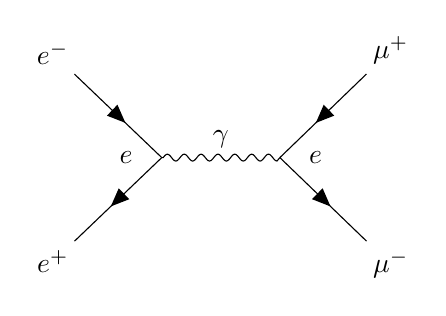
\begin{tikzpicture}
      \begin{feynman}
        \vertex (m1);
        \vertex [left=0.7em of m1] {$e$};
        \vertex [above left=of m1] (i1) {$e^-$};
        \vertex [below left=of m1] (i2) {$e^+$};
        \vertex [right=of m1] (m2);
        \vertex [right=0.7em of m2] {$e$};
        \vertex [above right=of m2] (f2) {$\mu^+$};
        \vertex [below right=of m2] (f1){$\mu^-$};

        \diagram*{
          (i1) -- [fermion] (m1) -- [fermion] (i2),
          (f2) -- [fermion] (m2) -- [fermion] (f1),
          (m1) -- [photon, edge label=$\gamma$] (m2)
        };
      \end{feynman}
    \end{tikzpicture}
\end{center}
\item Can also have 'u-channel' (since identical particles in the final state). The `t-channel' gives
\begin{center}
    \begin{tikzpicture}
      \begin{feynman}
        \vertex (m1);
        \vertex [above=0.7 em of m1] {$e$};
        \vertex [above left= of m1](i1) {$e^+$};
        \vertex [above right= of m1](f1){$\gamma$};
        \vertex [below= of m1](m2);
        \vertex [below=0.7 em of m2] {$e$};
        \vertex [below right= of m2](f2){$\gamma$};
        \vertex [below left= of m2](i2){$e^-$};
        \diagram*{
          (f1) -- [photon] (m1) -- [fermion] (i1),
          (m2) -- [fermion, edge label=$e^\pm$] (m1),
          (i2) -- [fermion] (m2),
          (f2) -- [photon] (m2)
        };
      \end{feynman}
    \end{tikzpicture}
\end{center}
\item Photons cannot self-couple, so the propagator must be electrons and positrons.
\begin{center}
    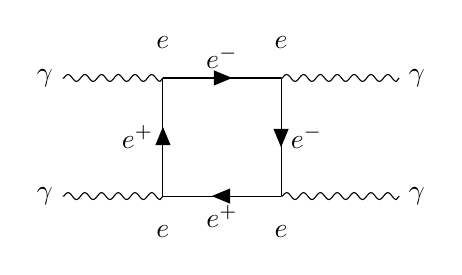
\begin{tikzpicture}
      \begin{feynman}
        \vertex (i1) {$\gamma$};
        \vertex [below=of i1] (i2) {$\gamma$};
        \vertex [right=of i1] (m1);
        \vertex [above=0.7 em of m1] {$e$};
        \vertex [right=of m1] (n1);
         \vertex [above=0.7 em of n1] {$e$};
        \vertex [right=of n1] (f1) {$\gamma$};
        \vertex [right=of i2] (m2);
         \vertex [below=0.7 em of m2] {$e$};
        \vertex [right=of m2] (n2);
         \vertex [below=0.7 em of n2] {$e$};
        \vertex [right=of n2] (f2) {$\gamma$};

        \diagram* {
          (i1) -- [photon] (m1),
          (i2) -- [photon] (m2),
          (n1) -- [photon] (f1),
          (n2) -- [photon] (f2),

          (n1) -- [fermion, edge label=$e^-$] (n2) -- [fermion, edge label=$e^+$] (m2) -- [fermion, edge label=$e^+$] (m1) -- [fermion, edge label=$e^-$] (n1);
        };
      \end{feynman}
    \end{tikzpicture}
  \end{center}
  Since the final state consists of identical particles, we have the `u-process'.
\end{enumerate}
\end{ans}
\newpage
\begin{qns}[$\pi^0$ decay]\leavevmode
\begin{enumerate}[label=(\alph*)]
\item The $\pi^0$ ($J^P = 0^−$) decays predominantly to $\gamma\gamma$ but is also seen to decay to $e^+e^-\gamma$ (“Dalitz decay”), to $e^+e^−e^+e^−$ and to $e^+e^−$ with branching fractions of 1.2\%, 3.2$\times10^{−5}$ and 2$\times10^{−7}$ respectively. Draw the leading order Feynman diagrams for each of these decays. Based on the coupling constants involved (ignoring propagator effects etc.), give rough estimates of the branching fractions for each decay.
\item The $\rho^0$ ($J^P = 1^−$) decays to $e^+e^−$ with a branching fraction of $4\times10^{-5}$. Draw the Feynman diagram for this decay and comment on the difference between the $\pi^0\rightarrow e^+e^−$ and $\rho^0\rightarrow e^+e^−$ partial widths.
\end{enumerate}
[The $\pi^0$ and $\rho^0$ lifetimes are $8.4\times 10^{−17}$ s and $4.4\times 10^{−24}$ s respectively.]
\end{qns}
\begin{ans}
Consider $\pi^0$ and $\rho^0$ to be $u\overline{u}$ (could have also been $d\overline{d}$ for $\pi^0$ meson but cross-section would be smaller due to smaller charge). In reality, $\rho^0$ is $\frac{1}{\sqrt{2}}(u\overline{u}-d\overline{d})$, hence its $J^P$ is $1^-$.
\begin{enumerate}[label=(\alph*)]
\item Remember to conserve charge and lepton number. The 4 processes are
\begin{itemize}
    \item $\pi^0\rightarrow\gamma\gamma$. One example of a leading order Feynman diagram is as follow:
    \begin{center}
    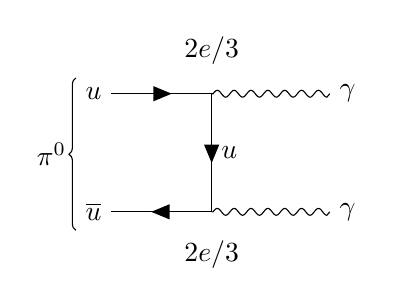
\begin{tikzpicture}
      \begin{feynman}
        \vertex (i1) {$u$};
        \vertex [below=of i1] (i2) {$\overline{u}$};
        \vertex [right=of i1] (m1);
        \vertex [above=0.7 em of m1] {$2e/3$};
        \vertex [right=of m1] (f1) {$\gamma$};
        \vertex [right=of i2] (m2);
        \vertex [below=0.7 em of m2] {$2e/3$};
        \vertex [right=of m2] (f2) {$\gamma$};

        \diagram* {
          (i1) -- [fermion] (m1),
          (m2) -- [fermion] (i2),
          (m1) -- [photon] (f1),
          (m2) -- [photon] (f2),

          (m1) -- [fermion, edge label=$u$] (m2);
        };
        \draw [decoration={brace}, decorate] (i2.south west) -- (i1.north west)
          node [pos=0.5, left] {$\pi^0$};
      \end{feynman}
    \end{tikzpicture}
  \end{center}
  The matrix element is $\mathcal{M}\propto4e^2/9$, and hence the cross-section is $\sigma\propto 16\alpha^2/81$.
  \item $\pi^0\rightarrow e^+e^-\gamma$. One example of a leading order Feynman diagram is as follow:
    \begin{center}
    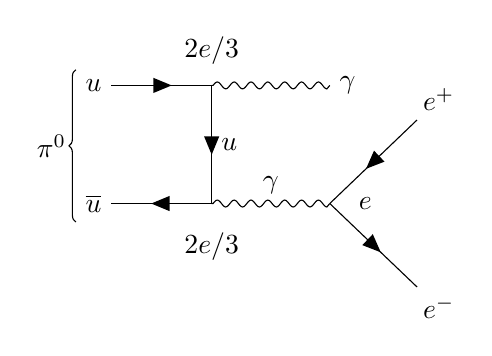
\begin{tikzpicture}
      \begin{feynman}
        \vertex (i1) {$u$};
        \vertex [below=of i1] (i2) {$\overline{u}$};
        \vertex [right=of i1] (m1);
        \vertex [above=0.4 em of m1] {$2e/3$};
        \vertex [right=of m1] (f1) {$\gamma$};
        \vertex [right=of i2] (m2);
        \vertex [below=0.7 em of m2] {$2e/3$};
        \vertex [right=of m2] (f2);
         \vertex [right=0.7 em of f2] {$e$};
        \vertex [above right=of f2] (f3) {$e^+$};
        \vertex [below right=of f2] (f4) {$e^-$};

        \diagram* {
          (i1) -- [fermion] (m1),
          (m2) -- [fermion] (i2),
          (m1) -- [photon] (f1),
          (m2) -- [photon, edge label=$\gamma$] (f2),
          (f3) -- [fermion] (f2),
          (f2) -- [fermion] (f4),
          (m1) -- [fermion, edge label=$u$] (m2);
        };
        \draw [decoration={brace}, decorate] (i2.south west) -- (i1.north west)
          node [pos=0.5, left] {$\pi^0$};
      \end{feynman}
    \end{tikzpicture}
  \end{center}
  Either photon may undergo the pair production, so the matrix element is $\mathcal{M}\propto2\times4e^3/9$, and hence the cross-section is $\sigma\propto4\times16\alpha^3/81$.
  \item $\pi^0\rightarrow e^+e^-e^+e^-$. One example of a leading order Feynman diagram is as follow:
    \begin{center}
    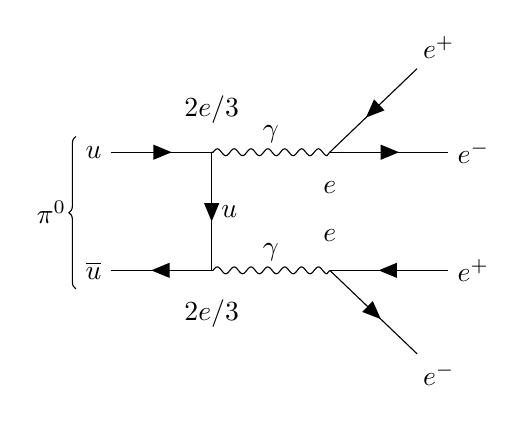
\begin{tikzpicture}
      \begin{feynman}
        \vertex (i1) {$u$};
        \vertex [below=of i1] (i2) {$\overline{u}$};
        \vertex [right=of i1] (m1);
        \vertex [above=0.7 em of m1] {$2e/3$};
        \vertex [right=of m1] (f1);
        \vertex [right=of i2] (m2);
        \vertex [below=0.7 em of m2] {$2e/3$};
        \vertex [right=of m2] (f2);
         \vertex [above=0.7 em of f2] {$e$};
        \vertex [right=of f2] (f3) {$e^+$};
        \vertex [below right=of f2] (f4) {$e^-$};
         \vertex [below=0.7 em of f1] {$e$};
        \vertex [above right=of f1] (f5) {$e^+$};
        \vertex [right=of f1] (f6) {$e^-$};

        \diagram* {
          (i1) -- [fermion] (m1),
          (m2) -- [fermion] (i2),
          (m1) -- [photon, edge label=$\gamma$] (f1),
          (m2) -- [photon, edge label=$\gamma$] (f2),
          (f3) -- [fermion] (f2),
          (f2) -- [fermion] (f4),
          (f5) -- [fermion] (f1),
          (f1) -- [fermion] (f6),
          (m1) -- [fermion, edge label=$u$] (m2);
        };
        \draw [decoration={brace}, decorate] (i2.south west) -- (i1.north west)
          node [pos=0.5, left] {$\pi^0$};
      \end{feynman}
    \end{tikzpicture}
  \end{center}
  The matrix element is $\mathcal{M}\propto4e^4/9$, and hence the cross-section is $\sigma\propto 16\alpha^4/81$.
  \item $\pi^0\rightarrow e^+e^-$. We cannot draw a vertex connecting the quark with a lepton. We must have a photon (QED) propagtor in between.
    \begin{center}
    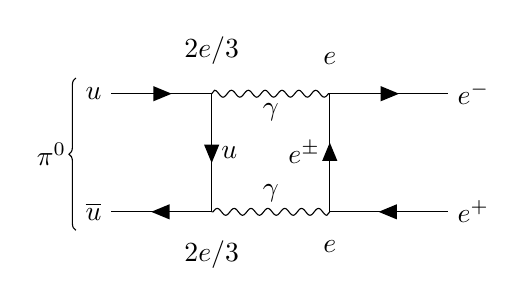
\begin{tikzpicture}
      \begin{feynman}
        \vertex (i1) {$u$};
        \vertex [below=of i1] (i2) {$\overline{u}$};
        \vertex [right=of i1] (m1);
        \vertex [above=0.7 em of m1] {$2e/3$};
        \vertex [right=of m1] (n1);
         \vertex [above=0.7 em of n1] {$e$};
        \vertex [right=of n1] (f1) {$e^-$};
        \vertex [right=of i2] (m2);
         \vertex [below=0.7 em of m2] {$2e/3$};
        \vertex [right=of m2] (n2);
         \vertex [below=0.7 em of n2] {$e$};
        \vertex [right=of n2] (f2) {$e^+$};

        \diagram* {
          (i1) -- [fermion] (m1),
          (m2) -- [fermion] (i2),
          (n1) -- [fermion] (f1),
          (f2) -- [fermion] (n2),

          (n2) -- [fermion, edge label=$e^\pm$] (n1) -- [photon, edge label=$\gamma$] (m1) -- [fermion, edge label=$u$] (m2) -- [photon, edge label=$\gamma$] (n2);
        };
        \draw [decoration={brace}, decorate] (i2.south west) -- (i1.north west)
          node [pos=0.5, left] {$\pi^0$};
      \end{feynman}
    \end{tikzpicture}
  \end{center}
  The matrix element is $\mathcal{M}\propto(2e^2/3)^2e^3$, and hence the cross-section is $\sigma\propto 16\alpha^5/81$.
\end{itemize}
The branching ratios are proportional to the ratio of cross-sections
$$1:4\alpha:\alpha^2:\alpha^3=1:0.029:5\times10^{-5}:3.9\times10^{-7}$$
where $\alpha=1/137$. This is consistent with the order of magnitude of the observed values.
\item For $\rho^0\rightarrow e^+e^-$, the s-channel is allowed with $\gamma$ being the propagator since $\rho^0$ has the same $J^P=1^-$ as the photon.
\begin{center}
    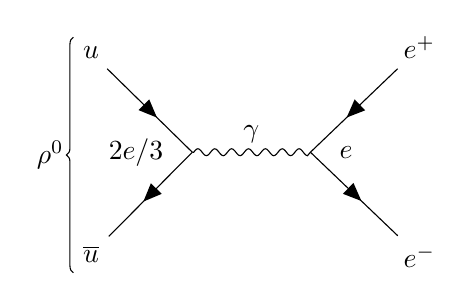
\begin{tikzpicture}
      \begin{feynman}
        \vertex (m1);
        \vertex [left=0.7em of m1] {$2e/3$};
        \vertex [above left=of m1] (i1) {$u$};
        \vertex [below left=of m1] (i2) {$\overline{u}$};
        \vertex [right=of m1] (m2);
        \vertex [right=0.7em of m2] {$e$};
        \vertex [above right=of m2] (f2) {$e^+$};
        \vertex [below right=of m2] (f1){$e^-$};

        \diagram*{
          (i1) -- [fermion] (m1) -- [fermion] (i2),
          (f2) -- [fermion] (m2) -- [fermion] (f1),
          (m1) -- [photon, edge label=$\gamma$] (m2)
        };
        \draw [decoration={brace}, decorate] (i2.south west) -- (i1.north west)
          node [pos=0.5, left] {$\rho^0$};
      \end{feynman}
    \end{tikzpicture}
\end{center}
The matrix element is $\mathcal{M}\propto 2e^2/3\implies\sigma\propto4\alpha^2/9$. The partial width is $w_i=B_i/\tau$ for $B_i$ the branching ratio and $\tau$ the half-life. The partial widths of $\rho$ and $\pi$ mesons are
$$w_\rho=\frac{6.6\times10^{-25}}{4.4\times10^{-24}}4\times10^{-5}=6~\text{keV},\quad w_\pi=\frac{6.6\times10^{-25}}{8.4\times10^{-17}}2\times10^{-7}=1.6~\mu \text{eV}$$
where we converted the half-life from SI units $s$ to natural units via $6.6\times10^{-25}$ GeV s. The ratio  of partial width is $10^9$ to 1. To account for the several orders of magnitude difference:
\begin{itemize}
    \item longer lifetime for $\pi^0$
    \item $\pi^0$ decays via higher-order processes (drawn in part a)
    \item more vertices involving quarks in $\pi^0$
    \item more propagators for $\pi^0$.
\end{itemize}
\end{enumerate}
\end{ans}
\newpage
\begin{qns}[Drell-Yan]
The Drell-Yan process, which is the production of charged lepton pairs in hadron-hadron interactions ($\pi N\rightarrow\mu^+\mu^-+$ anything, for example), proceeds via quark-antiquark annihilation into a single virtual photon. Draw a typical Feynman diagram for this process. Show that the Drell-Yan cross-sections in $\pi^+p$, $\pi^+n$, $\pi^-p$ and $\pi^-n$ interactions would be expected to be in the ratio 1 : 2 : 8 : 4.\\[5pt]
What would you expect to be the Drell-Yan cross-sections for $pp$ and $\overline{p}p$ collisions compared with the Drell-Yan cross-section for $\pi^+p$ interactions?
\end{qns}
\begin{ans}
The pion $\pi^+$ is $u\overline{d}$ while the pion $\pi^-$ is $d\overline{u}$.
\begin{enumerate}
    \item $\pi^+p$: We have $\mathcal{M}\propto e^2/3\implies\sigma\propto\alpha^2/9$.
    \begin{center}
    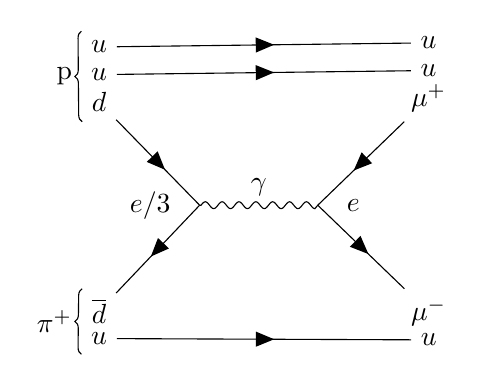
\begin{tikzpicture}
      \begin{feynman}
        \vertex (m1);
        \vertex [left=0.7em of m1] {$e/3$};
        \vertex [above left=of m1] (i1) {$d$};
        \vertex [above=1 em of i1] (si2) {$u$};
        \vertex [above=1 em of si2] (si1) {$u$};
        \vertex [below left=of m1] (i2) {$\overline{d}$};
        \vertex [below=1 em of i2] (si3) {$u$};
        \vertex [right=of m1] (m2);
        \vertex [right=0.7em of m2] {$e$};
        \vertex [above right=of m2] (f2) {$\mu^+$};
        \vertex [below right=of m2] (f1){$\mu^-$};
        \vertex [below=1 em of f1] (sf3) {$u$};
        \vertex [above=1 em of f2] (sf2) {$u$};
        \vertex [above=1 em of sf2] (sf1) {$u$};
        \diagram*{
          (i1) -- [fermion] (m1) -- [fermion] (i2),
          (f2) -- [fermion] (m2) -- [fermion] (f1),
          (m1) -- [photon, edge label=$\gamma$] (m2),
          (si1) -- [fermion] (sf1),
          (si2) -- [fermion] (sf2),
          (si3) -- [fermion] (sf3)
        };
        \draw [decoration={brace}, decorate] (i1.south west) -- (si1.north west)
          node [pos=0.5, left] {p};
          \draw [decoration={brace}, decorate] (si3.south west) -- (i2.north west)
          node [pos=0.5, left] {$\pi^+$};
      \end{feynman}
    \end{tikzpicture}
\end{center}

\item $\pi^+n$: There are two down quarks available for annihilation, so we have $\mathcal{M}\propto 2\times e^2/3\implies\sigma\propto(\alpha^2/9)+(\alpha^2/9)=2\alpha^2/9$.
    \begin{center}
    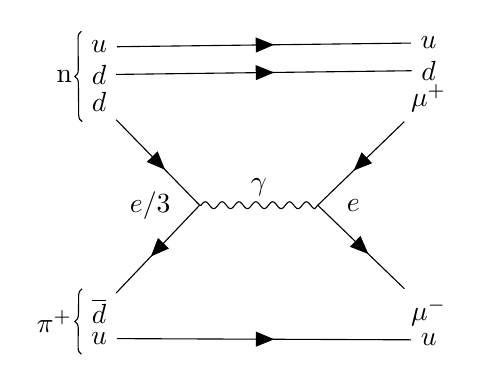
\begin{tikzpicture}
      \begin{feynman}
        \vertex (m1);
        \vertex [left=0.7em of m1] {$e/3$};
        \vertex [above left=of m1] (i1) {$d$};
        \vertex [above= 1 em of i1] (si2) {$d$};
        \vertex [above=1 em of si2] (si1) {$u$};
        \vertex [below left=of m1] (i2) {$\overline{d}$};
        \vertex [below=1 em of i2] (si3) {$u$};
        \vertex [right=of m1] (m2);
        \vertex [right=0.7em of m2] {$e$};
        \vertex [above right=of m2] (f2) {$\mu^+$};
        \vertex [below right=of m2] (f1){$\mu^-$};
        \vertex [below=1 em of f1] (sf3) {$u$};
        \vertex [above=1 em of f2] (sf2) {$d$};
        \vertex [above=1 em of sf2] (sf1) {$u$};
        \diagram*{
          (i1) -- [fermion] (m1) -- [fermion] (i2),
          (f2) -- [fermion] (m2) -- [fermion] (f1),
          (m1) -- [photon, edge label=$\gamma$] (m2),
          (si1) -- [fermion] (sf1),
          (si2) -- [fermion] (sf2),
          (si3) -- [fermion] (sf3)
        };
        \draw [decoration={brace}, decorate] (i1.south west) -- (si1.north west)
          node [pos=0.5, left] {n};
          \draw [decoration={brace}, decorate] (si3.south west) -- (i2.north west)
          node [pos=0.5, left] {$\pi^+$};
      \end{feynman}
    \end{tikzpicture}
\end{center}

\item $\pi^-p$: There are two up quarks available for annihilation, so we have $\mathcal{M}\propto 2(2e/3)\implies\sigma\propto2\times4\alpha^2/9$.
    \begin{center}
    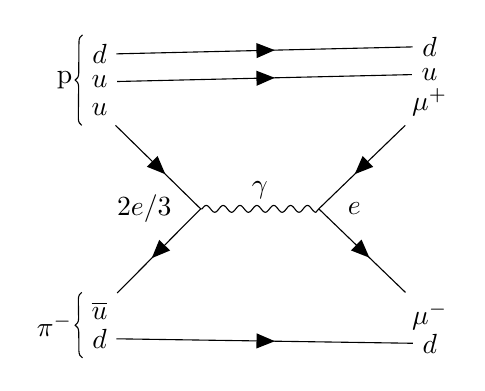
\begin{tikzpicture}
      \begin{feynman}
        \vertex (m1);
        \vertex [left=0.7em of m1] {$2e/3$};
        \vertex [above left=of m1] (i1) {$u$};
        \vertex [above=1 em of i1] (si2) {$u$};
        \vertex [above=1 em of si2] (si1) {$d$};
        \vertex [below left=of m1] (i2) {$\overline{u}$};
        \vertex [below=1 em of i2] (si3) {$d$};
        \vertex [right=of m1] (m2);
        \vertex [right=0.7em of m2] {$e$};
        \vertex [above right=of m2] (f2) {$\mu^+$};
        \vertex [below right=of m2] (f1){$\mu^-$};
        \vertex [below=1 em of f1] (sf3) {$d$};
        \vertex [above=1 em of f2] (sf2) {$u$};
        \vertex [above=1 em of sf2] (sf1) {$d$};
        \diagram*{
          (i1) -- [fermion] (m1) -- [fermion] (i2),
          (f2) -- [fermion] (m2) -- [fermion] (f1),
          (m1) -- [photon, edge label=$\gamma$] (m2),
          (si1) -- [fermion] (sf1),
          (si2) -- [fermion] (sf2),
          (si3) -- [fermion] (sf3)
        };
        \draw [decoration={brace}, decorate] (i1.south west) -- (si1.north west)
          node [pos=0.5, left] {p};
          \draw [decoration={brace}, decorate] (si3.south west) -- (i2.north west)
          node [pos=0.5, left] {$\pi^-$};
      \end{feynman}
    \end{tikzpicture}
\end{center}
\item $\pi^-n$: 
We have $\mathcal{M}\propto 2e^2/3\implies\sigma\propto4\alpha^2/9$.
    \begin{center}
    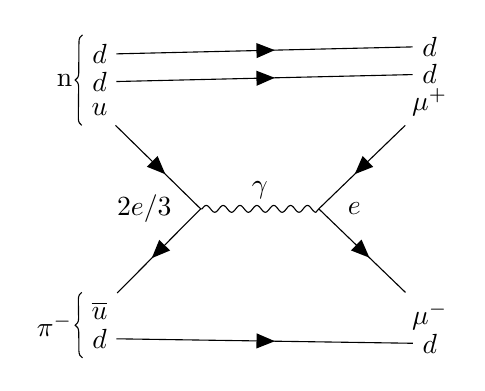
\begin{tikzpicture}
      \begin{feynman}
        \vertex (m1);
        \vertex [left=0.7em of m1] {$2e/3$};
        \vertex [above left=of m1] (i1) {$u$};
        \vertex [above=1 em of i1] (si2) {$d$};
        \vertex [above=1 em of si2] (si1) {$d$};
        \vertex [below left=of m1] (i2) {$\overline{u}$};
        \vertex [below= 1 em of i2] (si3) {$d$};
        \vertex [right=of m1] (m2);
        \vertex [right=0.7em of m2] {$e$};
        \vertex [above right=of m2] (f2) {$\mu^+$};
        \vertex [below right=of m2] (f1){$\mu^-$};
        \vertex [below=1 em of f1] (sf3) {$d$};
        \vertex [above=1 em of f2] (sf2) {$d$};
        \vertex [above=1 em of sf2] (sf1) {$d$};
        \diagram*{
          (i1) -- [fermion] (m1) -- [fermion] (i2),
          (f2) -- [fermion] (m2) -- [fermion] (f1),
          (m1) -- [photon, edge label=$\gamma$] (m2),
          (si1) -- [fermion] (sf1),
          (si2) -- [fermion] (sf2),
          (si3) -- [fermion] (sf3)
        };
        \draw [decoration={brace}, decorate] (i1.south west) -- (si1.north west)
          node [pos=0.5, left] {n};
          \draw [decoration={brace}, decorate] (si3.south west) -- (i2.north west)
          node [pos=0.5, left] {$\pi^-$};
      \end{feynman}
    \end{tikzpicture}
\end{center}
\end{enumerate}
In $pp$ scattering, there are no antiquarks, so the cross-section is zero to leading order (However, in higher orders in QCD, the gluons in the proton can create virtual $q\overline{q}$ pairs, giving a non-zero rate). In $p\overline{p}$ collisions, we have two pairs of $u\overline{u}$ and a pair of $d\overline{d}$, hence the rate should be $\propto\bigg(4\times\frac{2^2}{3^2}+\frac{1^2}{3^2}\bigg)=\frac{17}{9}$, i.e. 17 times larger than that of $\pi^+p$.
\end{ans}
\subsection*{QCD and the quark model}
\begin{qns}[Spin and Parity]
When $\pi^-$ mesons are stopped in deuterium they form “pionic atoms” ($\pi^−d$) which usually undergo transitions to an atomic s-state ($\ell=0$), where upon the capture reaction $\pi^-d\rightarrow nn$ occurs and destroys them. (The fact that capture normally occurs in an s-state is established from studies of the X-rays emitted in the transitions before capture). Given that the deuteron has spin-parity $J^P = 1^+$ and the pion has spin 0, show that these observations imply that the pion has negative intrinsic parity.
\end{qns}
\begin{ans}
Draw the usual table, comparing $J$ and $P$ for the initial and final states:
\begin{center}
\begin{tabular}{|l|l|l|}
\hline
  & initial     & final      \\
  \hline
$J^P$     & $0^{P_\pi}$, $1^+$     &
$\frac{1}{2}^+$, $\frac{1}{2}^+$     \\
\hline
$P$ & $(+1)P_\pi(-1)^{\ell=0}=P_\pi$ & $(+1)(+1)(-1)^L=P_\pi$ by conservation of parity \\
\hline
$J$& $0+1$ & $J=|L-1|,\dots,|L+1|=1$ by conservation of $J$\\
\hline
\end{tabular}
\end{center}
where $P=+1$ for $u$ and $d$ each, so the neutron has an overall $P=+1$. The possible $L$'s are $L=0,1,2$, and hence the possible $S=J-L$ values are 0 and 1. But neutrons are fermions so the RHS's wavefunction must be overall anti-symmetric under exchange. Recall $S=0$ spin singlet is anti-symmetric while $S=1$ spin triplet is symmetric, and that even $L$ gives symmetric spatial wavefunction, etc. The only allowed combination is $L=1$ and $S=1$. Hence, $P_\pi=-1$.
\end{ans}
\begin{qns}[Hadron masses]\leavevmode
\begin{enumerate}[label={(\alph*)}]
\item Verify the quark model predictions given in the lectures for the following meson masses:
\begin{center}
\begin{tabular}{|c|c|c|}
\hline
 Meson & Calculated (MeV)     & Observed (MeV)      \\
  \hline
$\pi$     & 140   & 138    \\
\hline
$K$ & 484 & 496 \\
\hline
$\eta$ & 559 & 549\\
\hline
$\rho$ & 780 & 776\\
\hline
$\omega$ & 780 & 783\\
\hline
$K^*$ & 896 & 892\\
\hline
$\phi$ & 1032 & 1020\\
\hline
\end{tabular}
\end{center}
[Assume $m_u=m_d=$310 MeV, $m_s=$483 MeV and that the spin-spin interaction coefficient $A=0.0615$ GeV$^3$ in this case.]\\[5pt]
What would the model predict for the mass of the $\eta'$ meson (measured mass 958 MeV)?
\item  What must be the total spin of any pair of quarks in the baryons in the $J^P=\frac{3}{2}^+$ decuplet? Hence predict the masses of the decuplet baryons and compare your predictions with the measured values.\\[5pt]
[Assume in this case $m_u=m_d=$360 MeV, $m_s=$540 MeV and that the spin-spin interaction coefficient $A=0.026$ GeV$^3$ in this case.]
\end{enumerate}
\end{qns}
\begin{ans}\leavevmode
\begin{enumerate}[label={(\alph*)}]
\item Use the formula, noting that $A$ should be converted to units of MeV$^3$.
$$M=m_1+m_2+\frac{A}{m_1m_2}\bigg[\frac{1}{2}J(J+1)-\frac{3}{4}\bigg]$$
The corresponding table for the mesons will be
\begin{center}
\begin{tabular}{|c|c|c|c|c|}
\hline
 Meson & $J^P$ & Composition & Calculated (MeV)     & Observed (MeV)     \\
  \hline
$\pi$ & $0^-$ & u$\overline{u}$/d$\overline{d}$/u$\overline{d}$/d$\overline{u}$   & $310\times 2+\frac{0.0615(*10^3)^3}{310^2}(0.5(0)(1)-0.75)=140$   & 138   \\
\hline
$K$ & $0^-$ & d$\overline{s}$/u$\overline{s}$/s$\overline{u}$/s$\overline{d}$ & $310+483+\frac{0.0615(*10^3)^3}{310(483)}(0.5(0)(1)-0.75)=485$ & 496 \\
\hline
$\eta$ & $0^-$&$\frac{1}{\sqrt{6}}(u\overline{u}+d\overline{d}-2s\overline{s})$& see below & 549  \\
\hline
$\rho$ & $1^-$ & u$\overline{u}$/d$\overline{d}$/u$\overline{d}$/d$\overline{u}$ & $310\times 2+\frac{0.0615(*10^3)^3}{310^2}(0.5(2)(1)-0.75)=780$ & 776  \\
\hline
$\omega$ & $1^-$ & $\frac{1}{\sqrt{2}}(u\overline{u}+d\overline{d})$ & $\frac{2}{2}(310\times 2+\frac{0.0615(*10^3)^3}{310^2}(0.5(2)(1)-0.75))=780$ & 783 \\
\hline
$K^*$ & $1^-$ & d$\overline{s}$/u$\overline{s}$/s$\overline{u}$/s$\overline{d}$ & $310+483+\frac{0.0615(*10^3)^3}{310(483)}(0.5(1)(1)-0.75)=896$ & 892 \\
\hline
$\phi$ & $1^-$ & s$\overline{s}$ & $483\times 2+\frac{0.0615(*10^3)^3}{483^2}(0.5(2)(1)-0.75)=1031.9$ & 1020  \\
\hline
\end{tabular}
\end{center}
where we have to include the linear combination coefficients in the computation of the masses. For $\eta$,
$$\frac{1}{6}\bigg(2\times 310-\frac{3(0.0615\times10^9)}{4(310)^2}\bigg)+\frac{1}{6}\bigg(2\times 310-\frac{3(0.0615\times10^9)}{4(310)^2}\bigg)+\frac{2^2}{6}\bigg(2\times 483-\frac{3\times 0.0615\times10^9}{4\times 483^2}\bigg)=558.9~\text{MeV}$$
$\eta'$ has $J^P=0^-$ and composition $\frac{1}{\sqrt{3}}(u\overline{u}+d\overline{d}+s\overline{s})$ and thus has mass
$$\frac{1}{3}\bigg(2\times 310-\frac{3(0.0615\times10^9)}{4(310)^2}\bigg)+\frac{1}{3}\bigg(2\times 310-\frac{3(0.0615\times10^9)}{4(310)^2}\bigg)+\frac{1}{3}\bigg(2\times 483-\frac{3\times 0.0615\times10^9}{4\times 483^2}\bigg)=349.4~\text{MeV}$$
which is significantly smaller than the measured mass of 958 MeV.
\item In a $J^P=\frac{3}{2}^+$ system, $J_{12}=1$ for any two quarks, in order for $J=\frac{3}{2}$ overall. Since $J=1$ for two spins, we have the eigenvalue for $\vec{s}~^2$ to be $s(s+1)$ and thus
$$\vec{s}_1\cdot\vec{s}_2=\frac{1}{2}(|\vec{s}|^2-|\vec{s}_1|^2-|\vec{s}_2|^2)=\frac{1}{2}(1(1+1)-(0.5)(0.5+1)-(0.5)(0.5+1))=\frac{1}{4}$$
Hence, the total mass of the decuplet baryons is
$$M=m_1+m_2+m_3+\frac{A'}{4}\bigg(\frac{1}{m_1m_2}+\frac{1}{m_1m_3}+\frac{1}{m_2m_3}\bigg)$$
with $A'=0.026(*10^3)^3$ MeV.
\begin{center}
\begin{tabular}{|c|c|c|c|}
\hline
 Baryon & Composition & Calculated (MeV)     & Observed (MeV)     \\
  \hline
$\Delta$     & ddd/udd/uud/uuu   & $360\times 3+\frac{0.026(*10^3)^3}{4}\frac{3}{360^2}=1230$  & 1232  \\
\hline
$\Sigma$     & dds/uds/uus   & $360\times 2+540+\frac{0.026(*10^3)^3}{4}\bigg(\frac{1}{360^2}+\frac{2}{360(540)}\bigg)=1377$  & 1385  \\
\hline
$\Xi$     & dss/uss   & $540\times 2+360+\frac{0.026(*10^3)^3}{4}\bigg(\frac{1}{540^2}+\frac{2}{360(540)}\bigg)=1529.2$  & 1533  \\
\hline
$\Omega$     & sss   & $540\times 3+\frac{0.026(*10^3)^3}{4}\frac{3}{540^2}=1686.9$  & 1672.5  \\
\hline
\end{tabular}
\end{center}
The deviations with the measured masses are small.
\end{enumerate}
\end{ans}
\newpage
\begin{qns}[$p$ and $n$ moments]
Derive the magnetic moments of the proton and neutron in the quark model as follows:
\begin{enumerate}[label={(\alph*)}]
    \item Assuming all the quarks are in $\ell=0$ states what must be the total spin of the two u quarks in the proton? (Give reasons for your answer).
    \item Hence show that the wave function for a proton in the $s_z=+\frac{1}{2}$ state can be written as
    $$\frac{1}{\sqrt{6}}(2u\uparrow u\uparrow d\downarrow -u\uparrow u\downarrow d\uparrow -u\downarrow u\uparrow d\uparrow)$$
    and derive a similar expression for the neutron.
    \item Assuming $u$ and $d$ quarks have equal mass, write their magnetic moments in terms of this quark mass.
    \item Hence predict the ratio of the proton and neutron magnetic moments. Compare with the observed values: $\mu_p$ = 2.79 $\mu_N$ , $\mu_n$ = −1.91$\mu_N$. What value for the quark mass is needed to give these values? Is this sensible?
    \item Consider now the magnetic moments of the $\Sigma^+$ (uus) and $\Sigma^-$ (dds) baryons, which are also members of the spin-$\frac{1}{2}$ octet. Show that
$$\mu_{\Sigma^+}-\mu_{\Sigma^-}=\frac{4}{5}(\mu_p-\mu_n)$$
Test using measured values: $\mu_{\Sigma^+}$ = 2.458 $\pm$ 0.010$\mu_N$ , $\mu_{\Sigma^-}$ = −1.160 $\pm$ 0.025$\mu_N$.
\end{enumerate}
\end{qns}
\begin{ans}\leavevmode
\begin{enumerate}[label={(\alph*)}]
\item Since $\ell=0$, $\psi_{\text{space}}$ is symmetric under exchange. Since the quark composition is $uu$, $\psi_{\text{flavour}}$ is symmetric under exchange. Hadrons are colour singlets, so $\psi_{\text{colour}}$ will be anti-symmetric under exchange. Since the proton is a fermion and has an overall wavefunction that is anti-symmetric under exchange, the spin wavefunction $\psi_{\text{spin}}$ is symmetric under exchange, with $S_{\text{uu}}=1$.
\item We have $qqq$ but from part (a), the first two quarks $qq$ are fixed to be spin symmetric. For $q_{s_1}q_{s_2}$ to be symmetric, we either have 
$$\uparrow\uparrow = |1,1\rangle_{s_1s_2},\quad\frac{1}{\sqrt{2}}(\uparrow\downarrow+\downarrow\uparrow)=|1,0\rangle_{s_1s_2}$$
For an overall $|\frac{1}{2},\frac{1}{2}\rangle_{s_1s_2s_3}$ baryon that has the first two spins symmetric under exchange, it must be a linear combination of the two possible cases:
\begin{itemize}
    \item 
    $$q_{s_1}:~\uparrow\quad q_{s_2}:~\uparrow\quad q_{s_3}:~\downarrow\implies|1,1\rangle_{s_1s_2}|0.5,-0.5\rangle_{s_3}$$
    \item 
    $$q_{s_1},~q_{s_2}:~\frac{1}{\sqrt{2}}(\uparrow\downarrow+\downarrow\uparrow)\quad q_{s_3}:~\uparrow\implies|1,0\rangle_{s_1s_2}|0.5,0.5\rangle_{s_3}$$
\end{itemize}
Consider $J_+|0.5,0.5\rangle_{s_1s_2s_3}=0$, then
\begin{align}
0&=J_+|0.5,0.5\rangle_{s_1s_2s_3}\nonumber\\&=c_1\bigg[J_+|1,1\rangle_{s_1s_2}|0.5,-0.5\rangle_{s_3}+|1,1\rangle_{s_1s_2} J_+|0.5,-0.5\rangle_{s_3}\bigg]+c_2\bigg[J_+|1,0\rangle_{s_1s_2}|0.5,0.5\rangle_{s_3}+|1,0\rangle_{s_1s_2} J_+|0.5,0.5\rangle_{s_3}\bigg]\nonumber\\&=c_1|1,1\rangle_{s_1s_2}|0.5,0.5\rangle_{s_3}+\sqrt{2}c_2|1,1\rangle_{s_1s_2}|0.5,0.5\rangle_{s_3}\implies c_1=-\sqrt{2}c_2\nonumber
\end{align}
But the state $|0.5,0.5\rangle_{s_1s_2s_3}$ is normalized, so $c_1^2+c_2^2=1\implies c_1=\sqrt{2/3}$ and $c_2=-\sqrt{1/3}$. We then obtain our result. Similarly, the overall $|0.5,-0.5\rangle_{s_1s_2s_3}$ baryon ($s_z=-1/2$) will be
$$\frac{1}{\sqrt{6}}(2u\downarrow u\downarrow d\uparrow -u\downarrow u\uparrow d\downarrow -u\uparrow u\downarrow d\downarrow)$$
Both states are symmetric under the exchange of $s_1$ and $s_2$. For the neutron, we simply do $u\leftrightarrow d$. The $s_z=\frac{1}{2}$ state will be
$$\frac{1}{\sqrt{6}}(2d\uparrow d\uparrow u\downarrow -d\uparrow d\downarrow u\uparrow -d\downarrow d\uparrow u\uparrow)$$
\item We have $\hat{\mu}_i=\frac{q_i}{m_i}\hat{S}_z$, where $\langle\hat{S}_z\rangle=\frac{\hbar}{2}$. Assume $m_u=m_d$, the magnetic moments for the up and down quarks respectively will be
$$\mu_u=\frac{2e}{3}\frac{\hbar}{2}\frac{1}{m}=\frac{\hbar e}{3m},\quad\mu_d=\frac{-1e}{3}\frac{\hbar}{2}\frac{1}{m}=-\frac{\hbar e}{6m}$$
\item The ratio will be
$$\frac{\mu_p}{\mu_n}=\frac{\langle\psi_{\text{spin}}(p)|2\hat{\mu}_u+\hat{\mu}_d|\psi_{\text{spin}}(p)\rangle}{\langle\psi_{\text{spin}}(n)|2\hat{\mu}_d+\hat{\mu}_u|\psi_{\text{spin}}(n)\rangle}$$
We have 
\begin{align}
    \mu_p&=\bigg(\frac{2}{\sqrt{6}}\bigg)^2(\mu_u+\mu_u-\mu_d)+\bigg(\frac{1}{\sqrt{6}}\bigg)^2(\mu_u-\mu_u+\mu_d)+\bigg(\frac{1}{\sqrt{6}}\bigg)^2(-\mu_u+\mu_u+\mu_d)\nonumber\\&=\frac{4}{3}\frac{\hbar e}{3m}+\frac{1}{3}\frac{\hbar e}{6m}\nonumber\\&=\frac{\hbar e}{2m}\nonumber
\end{align}
\begin{align}
    \mu_n&=\bigg(\frac{2}{\sqrt{6}}\bigg)^2(\mu_d+\mu_d-\mu_u)+\bigg(\frac{1}{\sqrt{6}}\bigg)^2(\mu_d-\mu_d+\mu_u)+\bigg(\frac{1}{\sqrt{6}}\bigg)^2(-\mu_d+\mu_d+\mu_u)\nonumber\\&=\frac{4}{3}\frac{\hbar e}{6m}+\frac{1}{3}\frac{\hbar e}{3m}\nonumber\\&=-\frac{\hbar e}{3m}\nonumber
\end{align}
Their ratio will be $-1.5$, quite close to the observed value $2.79/-1.91=-1.46$. We have $\mu_N=\frac{e\hbar}{2m_p}$, so
$$-1.91\mu_N=\mu_n=-\frac{2}{3}\frac{\hbar e}{2m}\implies\frac{m}{m_p}=\frac{2}{3(1.91)}\implies m=327MeV$$
where $m_p=938$ MeV in natural units. Similarly,
$$2.79\mu_N=\mu_p=\frac{\hbar e}{2m}\implies\frac{m}{m_p}=\frac{1}{2.79}\implies m=336MeV$$
\item Analogous to how we did it for $p$ and $n$,
$$\mu_{\Sigma^+}=\frac{4}{3}\mu_u-\frac{1}{3}\mu_s=\bigg(\frac{4}{3}\frac{1}{3}+\frac{1}{3}\frac{1}{6}\bigg)\frac{\hbar e}{m}=\frac{\hbar e}{2m},\quad\mu_{\Sigma^-}=\frac{4}{3}\mu_d-\frac{1}{3}\mu_s=\bigg(-\frac{4}{3}\frac{1}{6}+\frac{1}{3}\frac{1}{6}\bigg)\frac{\hbar e}{m}=-\frac{\hbar e}{6m}$$
but $\mu_u=\frac{\hbar e}{3m}$, $\mu_d=-\frac{e\hbar}{6m}$ and $\mu_s=-\frac{\hbar e}{6m}$. So, $\mu_{\Sigma^+}-\mu_{\Sigma^-}=\frac{\hbar e}{m}(0.5+(1/6))=\frac{2\hbar e}{3m}$ and $\mu_p-\mu_n=\frac{\hbar e}{m}(0.5+(1/3))=\frac{5\hbar e}{6m}$. The ratio will then be $4/5$. Experimentally, $\mu_{\Sigma^+}-\mu_{\Sigma^-}=(2.458-(-1.160))\mu_N=3.618\mu_N$ with a combined error of 0.027 $\mu_N$. $\mu_p-\mu_n=4.7\mu_N$. So the ratio is about 0.769.
\end{enumerate}
\end{ans}
\newpage
\begin{qns}[$\rho^0$ Decay]
Consider the decay of the $\rho^0$ meson ($J^P=1^-$) in the following decay modes:
\begin{enumerate}[label={(\alph*)}]
\item $\rho^0\rightarrow\pi^0\gamma$
\item $\rho^0\rightarrow\pi^+\pi^-$
\item $\rho^0\rightarrow\pi^0\pi^0$
\item $\rho^0\rightarrow e^+e^-$
\end{enumerate}
In each case, draw an appropriate Feynman diagram and determine whether the process is allowed or forbidden. By considering the strength of the forces involved, list the decay modes in order of expected rate.\\[5pt]
The ratio of partial widths $\Gamma(\rho^0\rightarrow\pi^0\gamma)/\Gamma(\omega^0\rightarrow\pi^0\gamma)$ is approximately 0.1 while the ratio $\Gamma(\rho^0\rightarrow e^+e^-)/\Gamma(\omega^0\rightarrow e^+e^-)$ is approximately 10. Suggest an explanation for these observations.\\[5pt]
[The quark wavefunctions for the mesons are $\frac{1}{\sqrt{2}}[u\overline{u}-d\overline{d}]$ for both $\pi^0$ and for $\rho^0$, and $\frac{1}{\sqrt{2}}[u\overline{u}+d\overline{d}]$ for $\omega^0$.]
\end{qns}
\begin{ans}\leavevmode
\begin{enumerate}[label={(\alph*)}]
\item $\rho^0\rightarrow\pi^0\gamma$: Take $\rho^0$ and $\pi^0$ to have composition $u\overline{u}$.
\begin{center}
    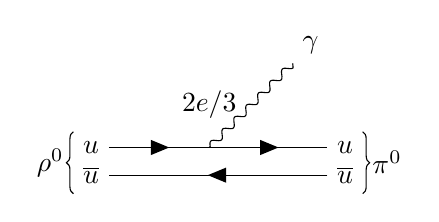
\begin{tikzpicture}
      \begin{feynman}
        \vertex (i1) {$u$};
        \vertex [below= 1 em of i1] (i2) {$\overline{u}$};
        \vertex [right=of i1] (m1);
        \vertex [above=0.7 em of m1] {$2e/3$};
        \vertex [above right=of m1] (f1) {$\gamma$};
        \vertex [right=of m1] (f2) {$u$};
        \vertex [right=of i2] (m2);
        \vertex [below =1em of f2] (f3) {$\overline{u}$};
        \diagram* {
          (i1) -- [fermion] (m1),
          (f3) -- [fermion] (i2),
          (m1) -- [photon] (f1),
          (m1) -- [fermion] (f2)
        };
        \draw [decoration={brace}, decorate] (i2.south west) -- (i1.north west)
          node [pos=0.5, left] {$\rho^0$};
          \draw [decoration={brace}, decorate] (f2.north east) -- (f3.south east)
          node [pos=0.5, right] {$\pi^0$};
      \end{feynman}
    \end{tikzpicture}

\begin{tabular}{|l|l|l|}
\hline
  & initial     & final      \\
  \hline
$J^P$     & $1^-$     &
$0^-$, $1^-$     \\
\hline
$P$ & $-1$ & $(-1)(-1)(-1)^L=-1$ \\
\hline
$J$& $0+1$ &need $J=|L-1|,\dots,|L+1|=1$ for conservation\\
\hline
\end{tabular}
\end{center}
The combined spin for the final state is $S=1$. By conservation of total angular momentum, $J=1$, we have $J=|L-1|,|L|,|L+1|=1\implies L=0,1,2$. But the final state is a fermion with overall anti-symmetric wavefunction, so we cannot have even $L$. Furthermore, we need $L=1$ to conserve parity, and this is consistent with conservation of $J$, i.e. $J=1$. This is an allowed process with $\mathcal{M}\propto 2e/3$.
\item $\rho^0\rightarrow\pi^+\pi^-$: Again, take $\rho^0$ to be $u\overline{u}$. $\pi^+$ and $\pi^-$ will be $u\overline{d}$ and $\overline{u}d$ respectively.
\begin{center}
    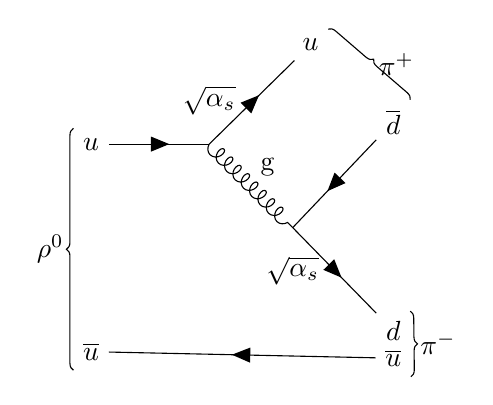
\begin{tikzpicture}
      \begin{feynman}
        \vertex (i1) {$u$};
       
        \vertex [right=of i1] (m1);
        \vertex [above=0.7 em of m1] {$\sqrt{\alpha_s}$};
        \vertex [above right=of m1] (f1) {$u$};
        \vertex [below right=of m1] (m3);
        \vertex [below=0.7 em of m3] {$\sqrt{\alpha_s}$};
        \vertex [above right=of m3] (f2) {$\overline{d}$};
        \vertex [below right=of m3] (f3) {$d$};
         \vertex [below= 7.5 em of i1] (i2) {$\overline{u}$};
        \vertex [right=of i2] (m2);
        \vertex [below=1 em of f3] (f4) {$\overline{u}$};
        \diagram* {
          (i1) -- [fermion] (m1),
          (f4) -- [fermion] (i2),
          (m1) -- [fermion] (f1),
          (m1) -- [gluon, edge label = g] (m3),
          (f2) -- [fermion] (m3),
          (m3) -- [fermion] (f3)
        };
        \draw [decoration={brace}, decorate] (i2.south west) -- (i1.north west)
          node [pos=0.5, left] {$\rho^0$};
          \draw [decoration={brace}, decorate] (f1.north east) -- (f2.north east)
          node [pos=0.5, right] {$\pi^+$};
          \draw [decoration={brace}, decorate](f3.north east)  -- (f4.south east)
          node [pos=0.5, right] {$\pi^-$};
          
      \end{feynman}
    \end{tikzpicture}

\begin{tabular}{|l|l|l|}
\hline
  & initial     & final      \\
  \hline
$J^P$     & $1^-$     &
$0^-$, $0^-$     \\
\hline
$P$ & $-1$ & $(-1)(-1)(-1)^L=-1$ \\
\hline
$J$& $0+1$ &need $|L-0|=1$ for conservation\\
\hline
\end{tabular}
\end{center}
We need $L=1$ to conserve parity, and this is consistent with conservation of $J$, i.e. $J=1$. This is an allowed process with $\mathcal{M}\propto\alpha_s$.
\newpage
\item $\rho^0\rightarrow\pi^0\pi^0$: Again, take $\rho^0$ and $\pi^0$ to be $u\overline{u}$.
\begin{center}
    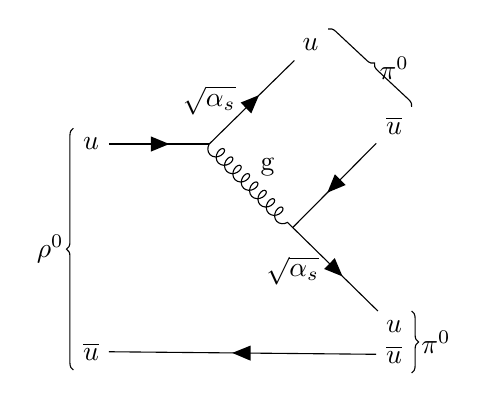
\begin{tikzpicture}
      \begin{feynman}
        \vertex (i1) {$u$};
       
        \vertex [right=of i1] (m1);
        \vertex [above=0.7 em of m1] {$\sqrt{\alpha_s}$};
        \vertex [above right=of m1] (f1) {$u$};
        \vertex [below right=of m1] (m3);
        \vertex [below=0.7 em of m3] {$\sqrt{\alpha_s}$};
        \vertex [above right=of m3] (f2) {$\overline{u}$};
        \vertex [below right=of m3] (f3) {$u$};
         \vertex [below= 7.5 em of i1] (i2) {$\overline{u}$};
        \vertex [right=of i2] (m2);
        \vertex [below= 1 em of f3] (f4) {$\overline{u}$};
        \diagram* {
          (i1) -- [fermion] (m1),
          (f4) -- [fermion] (i2),
          (m1) -- [fermion] (f1),
          (m1) -- [gluon, edge label = g] (m3),
          (f2) -- [fermion] (m3),
          (m3) -- [fermion] (f3)
        };
        \draw [decoration={brace}, decorate] (i2.south west) -- (i1.north west)
          node [pos=0.5, left] {$\rho^0$};
          \draw [decoration={brace}, decorate] (f1.north east) -- (f2.north east)
          node [pos=0.5, right] {$\pi^0$};
          \draw [decoration={brace}, decorate] (f3.north east) -- (f4.south east)
          node [pos=0.5, right] {$\pi^0$};
      \end{feynman}
    \end{tikzpicture}

\begin{tabular}{|l|l|l|}
\hline
  & initial     & final      \\
  \hline
$J^P$     & $1^-$     &
$0^-$, $0^-$     \\
\hline
$P$ & $-1$ & $(-1)(-1)(-1)^L=-1$ \\
\hline
$J$& $0+1$ &need $|L-0|=1$ for conservation\\
\hline
\end{tabular}
\end{center}
We need $L=1$ to conserve parity, and this is consistent with conservation of $J$, i.e. $J=1$. But, the final state consists of identical bosons. $\psi_{\text{flavour}}$ and $\psi_{\text{color}}$ are anti-symmetric, so $\psi_{\text{spin}}$ has to be symmetric in order for the overall wavefunction to be symmetric (bosons, of course assuming spatial wavefunction is symmetric), then $L$ must be even. This leads to a contradiction. This is a forbidden process with $\mathcal{M}\propto\alpha_s$.
\item $\rho^0\rightarrow e^+e^-$: $\rho^0$ and $\gamma$ have same $J^P=1^-$, so the reaction is allowed with $\mathcal{M}\propto\frac{2}{3}e^2$.
\begin{center}
    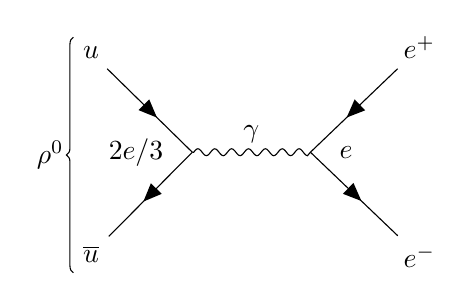
\begin{tikzpicture}
      \begin{feynman}
        \vertex (m1);
        \vertex [left=0.7em of m1] {$2e/3$};
        \vertex [above left=of m1] (i1) {$u$};
        \vertex [below left=of m1] (i2) {$\overline{u}$};
        \vertex [right=of m1] (m2);
        \vertex [right=0.7em of m2] {$e$};
        \vertex [above right=of m2] (f2) {$e^+$};
        \vertex [below right=of m2] (f1){$e^-$};

        \diagram*{
          (i1) -- [fermion] (m1) -- [fermion] (i2),
          (f2) -- [fermion] (m2) -- [fermion] (f1),
          (m1) -- [photon, edge label=$\gamma$] (m2)
        };
        \draw [decoration={brace}, decorate] (i2.south west) -- (i1.north west)
          node [pos=0.5, left] {$\rho^0$};
      \end{feynman}
    \end{tikzpicture}
\end{center}
\end{enumerate}
By looking at $\mathcal{M}$, the reactions in order of increasing rate: (d), (a) and (b), since $\alpha_s=1>>e=\frac{1}{137}$. Reaction (c) does not happen.\\[5pt]
The matrix element is obtained via
$$\mathcal{M}(i\rightarrow f)=\langle f|\hat{q}|i\rangle$$
where $\hat{q}$ is the charge operator. We have the ratio of partial widths to be
\begin{align}
\frac{\Gamma(\rho^0\rightarrow\pi^0\gamma)}{\Gamma(\omega^0\rightarrow\pi^0\gamma)}&=\frac{|\mathcal{M}(\rho^0\rightarrow\pi^0\gamma)|^2}{|\mathcal{M}(\omega^0\rightarrow\pi^0\gamma)|^2}\nonumber\\&=\frac{|\langle u\overline{u}-d\overline{d}|\hat{q}|u\overline{u}-d\overline{d}\rangle|^2}{|\langle u\overline{u}-d\overline{d}|\hat{q}|u\overline{u}+d\overline{d}\rangle|^2}\nonumber\\&=\frac{(2/3+(-1/3))^2}{(2/3-(-1/3))^2}=\frac{1}{9}\sim 0.1\nonumber
\end{align}
\begin{align}
\frac{\Gamma(\rho^0\rightarrow e^+e^-)}{\Gamma(\omega^0\rightarrow e^+e^-)}&=\frac{|\mathcal{M}(\rho^0\rightarrow e^+e^-)|^2}{|\mathcal{M}(\omega^0\rightarrow e^+e^-)|^2}\nonumber\\&=\frac{|\langle e^+e^-|\hat{q}|u\overline{u}-d\overline{d}\rangle|^2}{|\langle e^+e^-|\hat{q}|u\overline{u}+d\overline{d}\rangle|^2}\nonumber\\&=\frac{(2/3-(-1/3))^2}{(2/3+(-1/3))^2}=9\sim 10\nonumber
\end{align}
where $\langle u\overline{u}\pm d\overline{d}|\hat{q}|u\overline{u}\mp d\overline{d}\rangle=\langle u\overline{u}|q|u\overline{u}\rangle-\langle d\overline{d}|q|d\overline{d}\rangle$.
\end{ans}
\newpage
\begin{qns}[$J/\psi$ Meson]
The figure shown below (from Boyarski et al., Phys. Rev. Lett. 34 (1975) 1357) shows the original $e^+e^-$ annihilation cross-section measurements from the Mark II Collaboration which contributed to the discovery of the $J/\psi$ meson. The measurements were made during a fine scan of the $e^\pm$ beam energies at the SPEAR storage ring at SLAC which consisted of oppositely circulating $e^+$ and $e^-$ beams of equal energy. Figure (a) shows the cross-section for the process $e^+e^-\rightarrow$ hadrons, (b) shows the cross-section for $e^+e^-\rightarrow\mu^+\mu^-$ and (c) shows the cross-section for $e^+e^-\rightarrow e^+e^-$. The latter two were measured in a limited acceptance $|\cos\theta|<0.6$, where $\theta$ is the polar angle of the produced leptons.
\begin{figure}[H]
    \centering
    \includegraphics[scale=0.75]{PS2Q19.JPG}
\end{figure}
The observed width (a few MeV) of the $J/\psi$ resonance peak is predominantly caused by the energy spread inherent in the $e^+$, $e^−$ beams at each measured point. The relative centre-of mass energy between measurement points is however known very precisely (to about 1 part in $10^4$). The actual $J/\psi$ width is much smaller than the observed width, but can be extracted from the data as follows:
\begin{enumerate}[label={(\alph*)}]
\item The Breit-Wigner formula for the scattering of two particles of spin $s_1$ and $s_2$ in the region of a resonance of spin $J$ is:
$$\sigma(E)=\frac{\lambda^2}{4\pi}\frac{2J+1}{(2s_1+1)(2s_2+1)}\frac{\Gamma_i\Gamma_f}{[(E-E_0)^2+\Gamma^2/4]}$$
where $\lambda$ is the de Broglie wavelength of the incoming particles in the centre of mass frame, $E$ is the centre of mass energy, $E_0$ is the resonance energy, $\Gamma$ is the total width of the resonance and $\Gamma_i$ ($\Gamma_f$) is the partial width for decay into the initial (final) state. Show that, for the production of the $J/\psi$ resonance in $e^+e^-$ collisions, the integrated elastic cross-section under the resonance peak is given by
$$\sigma'=\int\sigma_{\text{el}}(E)dE\approx\frac{3}{8}\lambda^2B^2\Gamma$$
where $B$ is the branching fraction for the decay $J/\psi\rightarrow e^+e^-$.
\item Assume that, at each scan point, the beam energy spread produces a spread of centre of mass energies $E'$ distributed about the average centre of mass energy $E$ according to a probability distribution $f(E'-E)$. Show that the measured area under the resonance peak, $\int\sigma_{\text{meas}}(E)dE$, is equal to the true area under the peak, $\int\sigma(E)dE$.
\item  Given that the differential cross-section $d\sigma/d\Omega$ for the process $e^+e^-\rightarrow J/\psi\rightarrow e^+e^-$ is proportional to $1+\cos^2\theta$ where $\theta$ is the angle between the final $e^-$ and the beam direction, calculate the fraction of $J/\psi$ decays contained within the acceptance region $|\cos\theta|<0.6$ imposed for the $e^+e^-$ and $\mu^-\mu^+$ channels.
\item Use the data in the figure to estimate the quantities $\sigma'$ and $B$ defined above. You should obtain $\sigma'\sim$ 500 nb MeV and $B\sim$ 0.065 for the leptonic decays, after correcting for the limited acceptance. Hence estimate $\Gamma$ and $\Gamma_{\text{ee}}$ for the $J/\psi$.
\item The corresponding widths for the $\phi$ meson are $\Gamma=$4.4 MeV and $\Gamma_{\text{ee}}=$1.37 keV. Discuss why the $J/\psi$ and $\phi$ mesons have similar leptonic widths $\Gamma_{\text{ee}}$ but very different total widths $\Gamma$.
\end{enumerate}
\end{qns}
\begin{ans}\leavevmode
\begin{enumerate}[label={(\alph*)}]
\item We have $s_1=0.5=s_2$, $J=1$ and the branching ratio $\Gamma_i=\Gamma_f=B\Gamma$. The integrated elastic cross-section is
$$\sigma'=\int\sigma_{\text{el}}(E)dE=\frac{\lambda^2}{4\pi}\frac{3}{4}B^2\Gamma^2\int_{-\infty}^\infty\frac{1}{(E-E_0)^2+\Gamma^2/4}dE=\frac{\lambda^2}{4\pi}\frac{3}{4}\int_{-\pi/2}^{\pi/2}\frac{0.5\Gamma\sec^2\chi}{(1/4)\Gamma^2\sec^2\chi}d\chi=\frac{3}{8}\lambda^2B^2\Gamma$$
where we used the substitution $E-E_0=0.5\Gamma\tan\chi$ and that since $E_0>>\Gamma$, $-E_0$ may be assumed to be $-\infty$, hence the integration limit is $E\in[-E_0,\infty)\rightarrow(-\infty,\infty)$.
\item The measured cross-section is given by a convolution.
$$\int\sigma_{\text{meas}}(E)dE=\int\int f(E'-E)\sigma(E')dE'dE=\int\sigma(E)dE$$
where $\int f(E'-E)dE'=\int f(E'-E)dE=1$ by normalization.
\item We have
$$\sigma_{\text{tot}}=\int 1+\cos^2\theta d\Omega=\int_{-0.6}^{0.6}1+\cos^2\theta~d\cos\theta~\int_0^{2\pi}d\phi=2\pi\frac{8}{3}$$
Taking the ratio $\sigma/\sigma_{\text{tot}}=1.344/(8/3)=50.4\%$.
\item For Fig (a), (b) and (c) respectively, $\sigma_{\text{meas}}$ is $~(2230-30)=2200$ nb, $\sim(95-5)=90$ nb and $\sim(1355-55)=80$ nb above the background signal. For c), the integrated elastic cross-section $\sigma'\sim\frac{80nb}{0.504}\times0.003$ GeV, where the full width half maximum ($\Gamma_{\text{ee}}\sim$ 0.003 GeV). We thus have $\sigma'\sim$ 500 nb MeV. The branching fraction is taken to be the ratio of $\sigma_{\text{meas}}$:
$$B\sim\frac{80/0.504}{\frac{80+90}{0.504}+2200}=0.065$$
where we only need the correction factor (in part c) $0.504$ if $|\cos\theta|\leq 0.6$ (Fig b and c only). To find the widths, we need to first find the de Broglie wavelength which is
$$\lambda=\frac{h}{p}=\frac{2\pi}{0.5*3.095GeV}=2*2.03~\text{GeV}^{-1}=2*0.4~\text{fm}\implies\lambda^2=(2*0.4\times10^{-15})^210^{28}~\text{b}=4*0.16\times10^{-2}~\text{b}$$
expressed in natural units, where the momentum is for one incoming particle (half of the $J/\psi$ mass in the centre of mass frame). The total width is
$$\Gamma\sim\frac{8}{3}\frac{500 \text{nb}~\text{MeV}}{(0.8 \text{fm})^20.065^2}=\frac{8(500\times10^{-9}\text{b}~\text{MeV})}{3(0.64\times10^{-2}\text{b})0.065^2}=49~\text{keV}$$
The partial width is $\Gamma_{\text{ee}}=B\Gamma=0.065(49)=3.185$ keV.
\item The total width $\Gamma=4.4$ MeV for $\phi$ ($s\overline{s}$) is much greater than that of $J/\psi$ ($c\overline{c}$). This means $\phi$ has a shorter lifetime. This is because it may decay to a pair of Kaons $K^{\pm}$ ($u\overline{s}$). However, $c\overline{c}$ is kinematically inhibited from decaying to a pair of D mesons ($c\overline{d}$). The quarks must thus annihilate into 3 gulons. This complicated decay is `Zweig-suppressed' by the extra coupling constants and propagators needed.
\end{enumerate}
\end{ans}
\newpage
\section{Example Sheet 3}
\subsection*{Weak interaction}
\begin{qns}[Tau decay]
Draw a Feynman diagram for each of the principal decay modes of the $\tau^-$. Show that the $\tau$ lepton decay branching fractions should be approximately in the ratios
$$(\tau^-\rightarrow e^-\nu_\tau\overline{\nu}_e):(\tau^-\rightarrow \mu^-\nu_\tau\overline{\nu}_\mu):(\tau^-\rightarrow\text{hadrons})=1:1:3$$
The actual ratios are approximately 1.02 : 1 : 3.5. Suggest a possible explanation.\\[5pt]
Estimate the mean lifetime of the $\tau$ lepton, given that the branching fraction for $\tau^-\rightarrow e^-\overline{\nu}_e\nu_\tau$ is 18\%, and assume the total decay rate is given by Sargent’s Rule
$$\Gamma=\frac{G_F^2E_0^5}{60\pi^3}$$
[You may use $m_\tau=1.777$ GeV/c$^2$, $m_\mu=0.106$ GeV/c$^2$ and take the mean $\mu$ lifetime to be $2.197\times10^{-6}$s.]
\end{qns}
\begin{ans}\leavevmode
\begin{enumerate}
    \item $\tau^-\rightarrow e^-\nu_\tau\overline{\nu}_e$ with cross-section $\sigma\propto g_W^2$
    \begin{center}
    \begin{tikzpicture}
      \begin{feynman}
        \vertex (i1) {$\tau^-$};
        \vertex [right=of i1] (m1);
        \vertex [above=0.7 em of m1] {$g_W$};
        \vertex [above right=of m1] (f1) {$\nu_\tau$};
        \vertex [below right=of m1] (m3);
        \vertex [below=0.7 em of m3] {$g_W$};
        \vertex [above right=of m3] (f2) {$\overline{\nu}_e$};
        \vertex [below right=of m3] (f3) {$e^-$};
        \vertex [right=of i2] (m2);
        \diagram* {
          (i1) -- [fermion] (m1),
          (m1) -- [fermion] (f1),
          (m1) -- [photon, edge label = $W^-$] (m3),
          (f2) -- [fermion] (m3),
          (m3) -- [fermion] (f3)
        };
      \end{feynman}
    \end{tikzpicture}
    \end{center}
    \item $\tau^-\rightarrow \mu^-\nu_\tau\overline{\nu}_\mu$ with cross-section $\sigma\propto g_W^2$
    \begin{center}
    \begin{tikzpicture}
      \begin{feynman}
        \vertex (i1) {$\tau^-$};
        \vertex [right=of i1] (m1);
        \vertex [above=0.7 em of m1] {$g_W$};
        \vertex [above right=of m1] (f1) {$\nu_\tau$};
        \vertex [below right=of m1] (m3);
        \vertex [below=0.7 em of m3] {$g_W$};
        \vertex [above right=of m3] (f2) {$\overline{\nu}_\mu$};
        \vertex [below right=of m3] (f3) {$\mu^-$};
        \vertex [right=of i2] (m2);
        \diagram* {
          (i1) -- [fermion] (m1),
          (m1) -- [fermion] (f1),
          (m1) -- [photon, edge label = $W^-$] (m3),
          (f2) -- [fermion] (m3),
          (m3) -- [fermion] (f3)
        };
      \end{feynman}
    \end{tikzpicture}
    \end{center}
    \item $\tau^-\rightarrow \text{hadrons}$. Energy conservation does not permit $\tau$ to decay to heavier quarks, such as charm and hence only up, down and strange quarks. The cross-section for $d\overline{u}$ is $\sigma_{d\overline{u}}\propto3g_W^2V^2_{\text{du}}$ since there are 3 color combinations for $d\overline{u}$. Similarly, $\sigma_{s\overline{u}}\propto3g_W^2V^2_{\text{su}}$ since there are 3 colour combinations for $s\overline{u}$.
        \begin{center}
    \begin{tikzpicture}
      \begin{feynman}
        \vertex (i1) {$\tau^-$};
        \vertex [right=of i1] (m1);
        \vertex [above=0.7 em of m1] {$g_W$};
        \vertex [above right=of m1] (f1) {$\nu_\tau$};
        \vertex [below right=of m1] (m3);
        \vertex [below=0.7 em of m3] {$g_WV_{du}$};
        \vertex [below=1.8 em of m3] {$g_WV_{us}$};
        \vertex [above right=of m3] (f2) {$\overline{u}$};
        \vertex [below right=of m3] (f3) {$d,s$};
        \vertex [right=of i2] (m2);
        \diagram* {
          (i1) -- [fermion] (m1),
          (m1) -- [fermion] (f1),
          (m1) -- [photon, edge label = $W^-$] (m3),
          (f2) -- [fermion] (m3),
          (m3) -- [fermion] (f3)
        };
      \end{feynman}
    \end{tikzpicture}
    \end{center}
    With $V_{\text{du}}=\cos\theta_C>\sin\theta_C=V_{\text{su}}$ (crossings across different families are Cabibbo suppressed), the total cross-section is
    $$\sigma_{\text{hadrons}}=(\sigma_{d\overline{u}}+\sigma_{s\overline{u}})\propto 3g_W^2(\cos^2\theta_C+\sin^2\theta_C)\propto 3g_W^2$$
    The branching ratio is defined as
    $$B_f=\frac{\Gamma_f}{\Gamma_{\text{tot}}}=\frac{\sigma_f}{\sigma_{\text{tot}}}$$
    With the theoretical branching ratios to be
    $$B_{e^-\overline{\nu}_e}:B_{\mu^-\overline{\nu}_\mu}:B_{\text{hadrons}}=\sigma_{e^-\overline{\nu}_e}:\sigma_{\mu^-\overline{\nu}_\mu}:\sigma_{\text{hadrons}}=1:1:3$$
    Comparing this to the actual branching ratios 1.02: 1:3.5, this is reasonably close. The disparity occurs because
    \begin{itemize}
        \item electron production slightly favourable because $m_{e^-}<m_{\mu^-}$
        \item When hadrons are produced, gluons are exchanged. Since gluons may self-interact, they can produce virtual $q\overline{q}$ pairs. Such high order processes contribute to a larger cross-section.
    \end{itemize}
    Given that the branching fraction $B_\tau=\frac{\Gamma_{\tau\rightarrow e}}{\Gamma}$ for $\tau^-\rightarrow e^-\overline{\nu}_e\nu_\tau$ is 0.18, the mean lifetime of the $\tau$ lepton is
    $$\tau_\tau=\bigg(\frac{\Gamma_{\tau\rightarrow e}}{0.18}\bigg)^{-1}=0.18\frac{m_\mu^5}{m_\tau^5}\frac{1}{\Gamma_{\mu\rightarrow e}}=0.18\bigg(\frac{0.106\text{GeV/c}^2}{1.777\text{GeV/c}^2}\bigg)^5(2.197\times10^{-6}\text{s})=0.3~\text{ps}$$
    where we used Sargent's rule with energy proportional to the mass, i.e. $E_0\propto m$. Here, $\tau_\mu=\frac{1}{\Gamma_{\mu\rightarrow e}}$ as the branching ratio for the decay of $\mu^-\rightarrow e^-$ is 1.
\end{enumerate}
\end{ans}
\newpage
\begin{qns}[Threshold energy]
In a beam of antineutrinos, it is proposed to search for $\overline{\nu}_\tau$ via their interactions on nucleons in a stationary target to produce $\tau$-leptons.
\begin{enumerate}[label=(\alph*)]
\item Draw the Feynman diagram for the simplest such production process.
\item Calculate the minimum energy of the $\overline{\nu}_\tau$, which would permit $\tau$-lepton production.
\item What is the energy of the produced $\tau$-lepton when the $\overline{\nu}_\tau$ has this threshold energy?
\item How far will the $\tau$-lepton travel on average before decaying, given that its mean lifetime is 290 fs?
\end{enumerate}
[The masses of $\tau^+$, proton and neutron are 1.777 GeV/$c^2$, 0.938 GeV/$c^2$ and 0.9440 GeV/$c^2$ respectively.]
\end{qns}
\begin{ans}\leavevmode
\begin{enumerate}[label=(\alph*)]
\item The interactions on nucleons in a stationary target to produce $\tau$-leptons: $p+\overline{\nu}_\tau\rightarrow n+\tau^+$
\begin{center}
\begin{tikzpicture}
      \begin{feynman}
        \vertex (m1);
        \vertex [left=0.7em of m1] {$g_WV_{ud}$};
        \vertex [above left=of m1] (i1) {$u$};
        \vertex [above=1 em of i1] (si2) {$u$};
        \vertex [above=1 em of si2] (si1) {$d$};
        \vertex [below left=of m2] (i2) {$\overline{\nu}_\tau$};
        \vertex [below=of m1] (m2);
        \vertex [below=0.7em of m2] {$g_W$};
        \vertex [above right=of m1] (f2) {$d$};
        \vertex [below right=of m2] (f1){$\tau^+$};
        \vertex [above=1 em of f2] (sf2) {$u$};
        \vertex [above=1 em of sf2] (sf1) {$d$};
        \diagram*{
          (i1) -- [fermion] (m1) -- [fermion] (f2),
          (m2) -- [fermion] (i2),
          (f1) -- [fermion] (m2),
          (m1) -- [photon, edge label=$W^+$] (m2),
          (si1) -- [fermion] (sf1),
          (si2) -- [fermion] (sf2)
        };
        \draw [decoration={brace}, decorate] (i1.south west) -- (si1.north west)
          node [pos=0.5, left] {p};
        \draw [decoration={brace}, decorate] (sf1.north east) -- (f2.south east)
          node [pos=0.5, right] {n};
      \end{feynman}
    \end{tikzpicture}
\end{center}
where we conserved lepton number at the vertices.
\item The minimum energy required is that just enough to produce the products, i.e. $\sqrt{s}=m_\tau+m_n$ in the centre of momentum frame. $s$ is invariant so consider before the collision:
$$s=E^2-|p|^2=(E_\nu+E_p)^2-|p_\nu|^2=E_\nu^2+2E_\nu E_p+E_p^2-E_\nu^2=2E_\nu m_p+m_p^2$$
The minimum energy of the neutrino is
$$E_{\nu,\text{min}}=\frac{(m_\tau+m_n)^2-m_p^2}{2m_p}=\frac{(1.777\text{GeV/c}^2+0.940\text{GeV/c}^2)^2-(0.938\text{GeV/c}^2)^2}{2(0.938\text{GeV/c}^2)}=3.466~\text{GeV}$$
\item The Lorentz factor is
$$\gamma=\frac{E}{\sqrt{s}}=\frac{E_n+E_\tau}{m_n+m_\tau}=\frac{m_p+E_\nu}{m_n+m_\tau}=\frac{0.938~\text{GeV}+3.466~\text{GeV}}{0.940~\text{GeV}+1.777~\text{GeV}}=1.62$$
In the laboratory frame, the energy of the produced $\tau$ is
$$E_\tau=\gamma m_\tau c^2=1.62\times 1.777~\text{GeV/c}^2\times c^2=2.88\text{GeV}$$
\item In laboratory frame, the distance travelled is
$$\sqrt{\gamma^2-1}c\tau=\sqrt{1.62^2-1}(3\times10^8\text{m/s})(290\times10^{-15}\text{s})=111\mu\text{m}$$
\end{enumerate}
\end{ans}
\newpage
\begin{qns}[Omega Decay]
The $\Omega^-$ baryon (sss), produced in the event shown in Q.4 is seen to decay weakly through the decay chain $\Omega^-\rightarrow\Xi^0\pi^-$, $\Xi^0\rightarrow\Lambda^0\pi^0$ and $\Lambda^0\rightarrow p\pi^-$. Draw the Feynman diagrams for the decays of the $\Omega^-$, the $\Xi^0$ and the $\Lambda^0$.\\[5pt]
Draw a Feynman diagram for the strong decay $\Omega^-\rightarrow\Xi^-\overline{K^0}$ and explain why the decay is not observed. With the aid of a Feynman diagram explain why the weak decay $\Omega^-\rightarrow\Lambda^0\pi^-$ is strongly suppressed.\\[5pt]
[The strange hadrons have quark compositions and masses $\Omega^-$ (ss) 1.67 GeV, $\Xi^0$ (uss) 1.31 GeV, $\Xi^-$ (dss) 1.32 GeV, $\overline{K}^0$ (s$\overline{d}$) 498 MeV, $\Lambda^0$ (uds) 1.12 GeV]
\end{qns}
\begin{ans}\leavevmode
\begin{enumerate}
    \item $\Omega^-(\text{sss})\rightarrow\Xi^0(\text{uss})\pi^-(\overline{u}d)$
    \begin{center}
        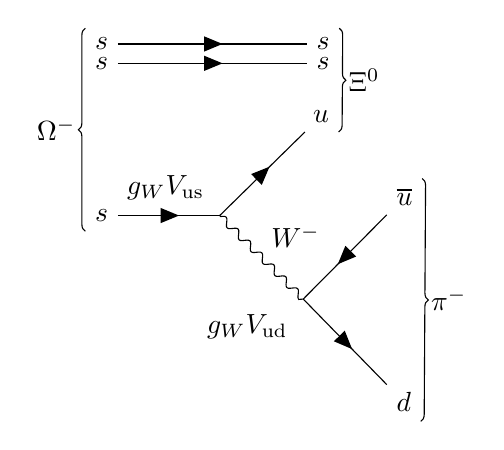
\begin{tikzpicture}
      \begin{feynman}
        \vertex (i1) {$s$};
        \vertex [right=of i1] (m1);
        \vertex [above left=0.3 em of m1] {$g_WV_{\text{us}}$};
        \vertex [above right=of m1] (f1) {$u$};
        \vertex [below right=of m1] (m3);
        \vertex [below left=0.3 em of m3] {$g_WV_{\text{ud}}$};
        \vertex [above right=of m3] (f2) {$\overline{u}$};
        \vertex [below right=of m3] (f3) {$d$};
         \vertex [above= 5.5 em of i1] (si1) {$s$};
        \vertex [right= 8 em of si1] (sf1) {$s$};
         \vertex [above= 0.7 em of si1] (si2) {$s$};
        \vertex [right= 8 em of si2] (sf2) {$s$};
        \diagram* {
          (i1) -- [fermion] (m1),
          (si1) -- [fermion] (sf1),
          (si2) -- [fermion] (sf2),
          (m1) -- [fermion] (f1),
          (m1) -- [photon, edge label = $W^-$] (m3),
          (f2) -- [fermion] (m3),
          (m3) -- [fermion] (f3)
        };
        \draw [decoration={brace}, decorate] (i1.south west) -- (si2.north west)
          node [pos=0.5, left] {$\Omega^-$};
        \draw [decoration={brace}, decorate] (sf2.north east) -- (f1.south east)
          node [pos=0.5, right] {$\Xi^0$};
           \draw [decoration={brace}, decorate] (f2.north east) -- (f3.south east)
          node [pos=0.5, right] {$\pi^-$};
      \end{feynman}
    \end{tikzpicture}
    \end{center}
    \item $\Xi^0(\text{uss})\rightarrow\Lambda^0(\text{uds})\pi^0(u\overline{u})$
        \begin{center}
        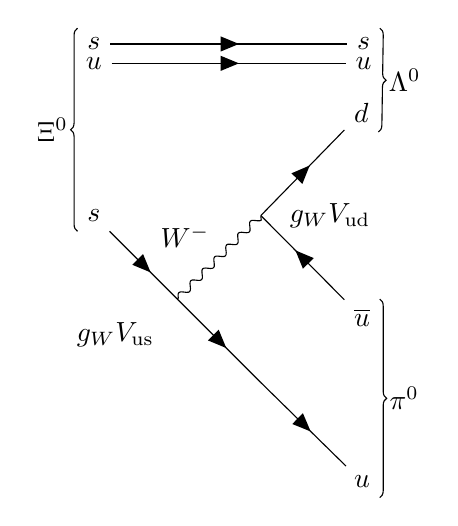
\begin{tikzpicture}
      \begin{feynman}
        \vertex (i1) {$s$};
        \vertex [below right=of i1] (m1);
        \vertex [below left=0.7 em of m1] {$g_WV_{\text{us}}$};
        \vertex [above right=of m1] (m3);
        \vertex [above right=of m3] (f1) {$d$};
        \vertex [right=0.7 em of m3] {$g_WV_{\text{ud}}$};
        \vertex [below right=of m3] (f2) {$\overline{u}$};
        \vertex [below right=of m1] (m4);
        \vertex [below right=of m4] (f3){$u$};
         \vertex [above= 5.5 em of i1] (si1) {$u$};
        \vertex [right= 9.75 em of si1] (sf1) {$u$};
         \vertex [above= 0.7 em of si1] (si2) {$s$};
        \vertex [right= 9.75 em of si2] (sf2) {$s$};
        \diagram* {
          (i1) -- [fermion] (m1)--[fermion](m4)--[fermion](f3),
          (si1) -- [fermion] (sf1),
          (si2) -- [fermion] (sf2),
          (m1) -- [photon, edge label = $W^-$] (m3),
          (f2) -- [fermion] (m3),
          (m3) -- [fermion] (f1)
        };
        \draw [decoration={brace}, decorate] (i1.south west) -- (si2.north west)
          node [pos=0.5, left] {$\Xi^0$};
        \draw [decoration={brace}, decorate] (sf2.north east) -- (f1.south east)
          node [pos=0.5, right] {$\Lambda^0$};
           \draw [decoration={brace}, decorate] (f2.north east) -- (f3.south east)
          node [pos=0.5, right] {$\pi^0$};
      \end{feynman}
    \end{tikzpicture}
    \end{center}
    \item $\Lambda^0(\text{uds})\rightarrow p(\text{uud})\pi^-(d\overline{u})$
      \begin{center}
        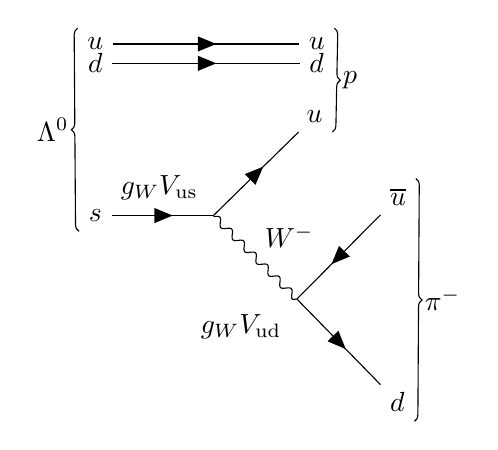
\begin{tikzpicture}
      \begin{feynman}
        \vertex (i1) {$s$};
        \vertex [right=of i1] (m1);
        \vertex [above left=0.3 em of m1] {$g_WV_{\text{us}}$};
        \vertex [above right=of m1] (f1) {$u$};
        \vertex [below right=of m1] (m3);
        \vertex [below left=0.3 em of m3] {$g_WV_{\text{ud}}$};
        \vertex [above right=of m3] (f2) {$\overline{u}$};
        \vertex [below right=of m3] (f3) {$d$};
         \vertex [above= 5.5 em of i1] (si1) {$d$};
        \vertex [right= 8 em of si1] (sf1) {$d$};
         \vertex [above= 0.7 em of si1] (si2) {$u$};
        \vertex [right= 8 em of si2] (sf2) {$u$};
        \diagram* {
          (i1) -- [fermion] (m1),
          (si1) -- [fermion] (sf1),
          (si2) -- [fermion] (sf2),
          (m1) -- [fermion] (f1),
          (m1) -- [photon, edge label = $W^-$] (m3),
          (f2) -- [fermion] (m3),
          (m3) -- [fermion] (f3)
        };
        \draw [decoration={brace}, decorate] (i1.south west) -- (si2.north west)
          node [pos=0.5, left] {$\Lambda^0$};
        \draw [decoration={brace}, decorate] (sf2.north east) -- (f1.south east)
          node [pos=0.5, right] {$p$};
           \draw [decoration={brace}, decorate] (f2.north east) -- (f3.south east)
          node [pos=0.5, right] {$\pi^-$};
      \end{feynman}
    \end{tikzpicture}
    \end{center}
\end{enumerate}
\newpage
$\Omega^-(\text{sss})\rightarrow\Xi^-(\text{dss})\overline{K}^0(s\overline{d})$ is a strong decay.
        \begin{center}
        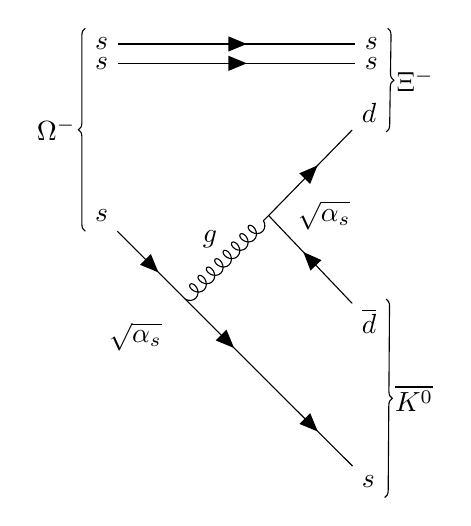
\begin{tikzpicture}
      \begin{feynman}
        \vertex (i1) {$s$};
        \vertex [below right=of i1] (m1);
        \vertex [below left=0.7 em of m1] {$\sqrt{\alpha_s}$};
        \vertex [above right=of m1] (m3);
        \vertex [above right=of m3] (f1) {$d$};
        \vertex [right=0.7 em of m3] {$\sqrt{\alpha_s}$};
        \vertex [below right=of m3] (f2) {$\overline{d}$};
        \vertex [below right=of m1] (m4);
        \vertex [below right=of m4] (f3) {$s$};
         \vertex [above= 5.5 em of i1] (si1) {$s$};
        \vertex [right= 9.75 em of si1] (sf1) {$s$};
         \vertex [above= 0.7 em of si1] (si2) {$s$};
        \vertex [right= 9.75 em of si2] (sf2) {$s$};
        \diagram* {
          (i1) -- [fermion] (m1)--[fermion] (m4)--[fermion](f3),
          (si1) -- [fermion] (sf1),
          (si2) -- [fermion] (sf2),
          (m1) -- [gluon, edge label = $g$] (m3),
          (f2) -- [fermion] (m3),
          (m3) -- [fermion] (f1)
        };
        \draw [decoration={brace}, decorate] (i1.south west) -- (si2.north west)
          node [pos=0.5, left] {$\Omega^-$};
        \draw [decoration={brace}, decorate] (sf2.north east) -- (f1.south east)
          node [pos=0.5, right] {$\Xi^-$};
           \draw [decoration={brace}, decorate] (f2.north east) -- (f3.south east)
          node [pos=0.5, right] {$\overline{K^0}$};
      \end{feynman}
    \end{tikzpicture}
    \end{center}
The minimum energy to obtain the products is
$$E_{\text{min}}=m_\Xi+m_{\overline{K^0}}=1.32~\text{GeV}+0.498~\text{GeV}=1.818~\text{GeV}$$
The centre of mass energy is, however, 
$$\sqrt{s}=m_\Omega=1.67~\text{GeV}<E_{\text{min}}$$
Hence, this strong decay is a kinematically forbidden process.\\[5pt]
Finally, for the reaction $\Omega^-(sss)\rightarrow\Lambda^0(uds)\pi^-(\overline{u}d)$,
       \begin{center}
        \begin{tikzpicture}
      \begin{feynman}
      \vertex (i1) {$s$};
         \vertex [above= 6.5 em of i1] (si1) {$s$};
        \vertex [right= 6 em of si1] (sf1) {$s$};
        \vertex [right =of i1](m1);
        \vertex [above left=0.7 em of m1] {$g_WV_{\text{su}}$};
        \vertex [above right =of m1](f1) {$u$};
        \vertex [below right =of m1](m2);
        \vertex [below left=0.5 em of m2] {$g_WV_{\text{ud}}$};
        \vertex [above right =of m2](f2){$d$};
        \vertex [below right =of m2](m3);
        \vertex [above right=0.7 em of m3] {$g_WV_{\text{us}}$};
        \vertex [below = 7.5 em of i1](i3){$s$};
        \vertex [below right= of m3](m4);
        \vertex [below left=0.7 em of m4] {$g_WV_{\text{ud}}$};
        \vertex [above right= of m4](f3){$d$};
        \vertex [below right= of m4](f4){$\overline{u}$};
        
        \diagram* {
        (si1) -- [fermion] (sf1),
        (i1) --[fermion] (m1)--[fermion] (f1),
        (m1) -- [photon, edge label =$W^-$] (m2),
        (m2) -- [fermion] (f2),
        (m3) -- [fermion,edge label=$\overline{u}$](m2),
        (i3) -- [fermion] (m3),
        (m3) -- [photon, edge label=$W^-$] (m4),
        (m4) --[fermion] (f3),
        (f4) -- [fermion](m4)
        };
         \draw [decoration={brace}, decorate] (i3.south west) -- (si2.north west)
          node [pos=0.5, left] {$\Omega^-$};
        \draw [decoration={brace}, decorate] (sf1.north east) -- (f2.south east)
          node [pos=0.5, right] {$\Lambda^0$};
           \draw [decoration={brace}, decorate] (f3.north east) -- (f4.south east)
          node [pos=0.5, right] {$\pi^-$};
      \end{feynman}
    \end{tikzpicture}
    \end{center}
    The matrix element is $\mathcal{M}\propto V_{\text{su}}^2V^2_{\text{ud}}g_W^4$. There are more vertices here since two strange quarks need to decay. The matrix element is doubly Cabibbo suppressed, hence this weak decay is strongly suppressed.
\end{ans}
\newpage
\subsection*{Electroweak Unification}
\begin{qns}[Z mass peak]\leavevmode
\begin{enumerate}[label=(\alph*)]
    \item  In lectures we deduced that the couplings of the Z boson to fermions should be of the form:
    $$g_Z[I_3-Q\sin^2\theta_W]\text{ where } g_Z=\frac{e}{\sin\theta_W\cos\theta_W}$$
    In this expression, $Q$ is the electric charge (in units of $e$), $I_3$ is the weak isospin of the fermion species and helicity state being considered and the weak mixing angle is given by $\sin^2\theta_W\approx 0.23$. The decay rate into $f\overline{f}$ (assumed massless compared with the Z) is proportional to ($g_L^2+g_R^2$) where $g_L$ and $g_R$ are the couplings to left-handed and righthanded fermions respectively. Compare the Z decay rates to pairs of charged lepton pairs of each species, neutrino-antineutrino pairs, and to u-like and d-like quark-antiquark pairs. Hence predict the branching fractions for Z decay to $\tau^+\tau^-$, to neutrinos and to hadrons.
    \item  In the OPAL experiment at LEP the cross-section for $e^+e^-\rightarrow\tau^+\tau^-$ was measured at various centre-of-mass energies. Some of the results are shown below. Plot these data
    \begin{center}
    \begin{tabular}{|c|c|}
    \hline
       $E_{\text{cm}}$/GeV  & $\sigma(e^+e^-\rightarrow\tau^+\tau^-)$/nb  \\
       \hline
        88.481 & 0.2769$\pm$ 0.0235\\
        \hline
        89.442 & 0.4892$\pm$ 0.0091\\
        \hline
        90.223 & $0.8331\pm0.0368$\\
        \hline
        91.283 & 1.4988$\pm$ 0.0213\\
        \hline
        91.969 & 1.1892$\pm$0.0235\\
        \hline
        92.971 & $0.7089\pm0.0105$\\
        \hline
        93.717 & 0.4989$\pm$0.0276\\
        \hline
    \end{tabular}
    \end{center}
    and make estimates of the Z boson mass, $m_Z$, the total width of the Z boson, $\Gamma_Z$, and the partial decay width to $\tau^+\tau^-$,$\Gamma_\tau$, (assuming lepton universality of the Neutral Current). Compare the branching fraction for $Z\rightarrow\tau^+\tau^-$ with your predictions from (a), and comment.\\[5pt]
    Why is the measured resonance curve asymmetric? Indicate what other effects need to be taken into account when accurately determining $m_Z$, $\Gamma_Z$ and $\Gamma_\tau$.
    \item Estimate the total decay width, $\Gamma_Z$, and the lifetime of the Z boson using the resonant cross-section ratio,
    $$\frac{\sigma(e^+e^-\rightarrow Z\rightarrow\text{hadrons})}{\sigma(e^+e^-\rightarrow Z\rightarrow\mu^+\mu^-)}=20.7$$
    and the measured values of the Z partial decay widths, $\Gamma(Z\rightarrow\mu^+\mu^-)=$ 83.3 MeV and $\Gamma(Z\rightarrow\nu_\mu\overline{\nu}_\mu)=$ 166.5 MeV. Make clear any assumptions you make.
\end{enumerate}
\end{qns}
\begin{ans}\leavevmode
\begin{enumerate}[label=(\alph*)]
\item The decay rates are $\Gamma\propto g_L^2+g_R^2$ where
$$g_L=g_Z(I_3-\sin^2\theta_W~Q),\quad g_R=-g_Z\sin^2\theta_W~Q,\quad\sin^2\theta_W\approx 0.23$$
where the right-handed $I_3=0$. We have:
\begin{center}
    \begin{tabular}{|c|c|c|}
    \hline
        $\ell$ & $Q$ & $I_3$ \\
          \hline
        LH & -1 & -1/2\\
         \hline
        RH & -1 & 0\\
        \hline
    \end{tabular}
    \begin{tabular}{|c|c|c|}
    \hline
        $\nu$ & $Q$ & $I_3$ \\
          \hline
        LH & 0 & +1/2\\
         \hline
        RH & 0 & 0\\
        \hline
    \end{tabular}
    \begin{tabular}{|c|c|c|}
    \hline
        $u,c$ & $Q$ & $I_3$ \\
          \hline
        LH & +2/3 & +1/2\\
         \hline
        RH & +2/3 & 0\\
        \hline
    \end{tabular}
    \begin{tabular}{|c|c|c|}
    \hline
        $d,s,b$ & $Q$ & $I_3$ \\
          \hline
        LH & -1/3 & -1/2\\
         \hline
        RH & -1/3 & 0\\
        \hline
    \end{tabular}
\end{center}
Their corresponding decay rates are
$$\Gamma_{\ell^+\ell^-}=g_Z^2((-0.5+0.23)^2+0.23^2)=0.1258g_Z^2,\quad\Gamma_{\nu\overline{\nu}}=g_Z^2(0.5^2)=0.25g_Z^2$$
for each charged lepton pair, and each neutrino pair respectively. The top quark is kinematically inhibited so for quarks with charge $2e/3$, we have:
$$\Gamma_{u\overline{u}}=\Gamma_{c\overline{c}}=3g_Z^2((0.5-0.23(2/3))^2+(0.23(2/3)^2))=0.4311g_Z^2$$
The bottom quark, although heavy, is not kinematically inhibited, so for quarks with charge $-e/3$ we have all 3 flavours:
$$\Gamma_{d\overline{d}}=\Gamma_{s\overline{s}}=\Gamma_{b\overline{b}}=3g_Z^2((-0.5+0.23(1/3))^2+(0.23(1/3))^2)=0.5553g_Z^2$$
The total decay rate is
$$\Gamma_{\text{tot}}=(3\times 0.1258+3\times 0.25+2\times0.4311+3\times 0.5553)g_Z^2=3.6555 g_Z^2$$
The branching fractions are
$$B_{\tau\tau^+}=\frac{\Gamma_{\tau\tau^+}}{\Gamma_{\text{tot}}}=\frac{0.1258}{3.6555}=0.034,\quad B_{\nu\overline{\nu}}=\frac{3\Gamma_{\nu\overline{\nu}}}{\Gamma_{\text{tot}}}=\frac{3(0.25)}{3.6555}=0.205$$
$$B_{\text{hadrons}}=\frac{2\Gamma_{u\overline{u}}+3\Gamma_{d\overline{d}}}{\Gamma_{\text{tot}}}=\frac{2\times 0.4311+3\times 0.5553}{3.6555}=0.6916$$
\item Plotting the data on Origin and fitting it to a Lorentzian shape:
\begin{figure}[H]
    \centering
    \includegraphics[width=0.7\linewidth]{Lorentzian.PNG}
\end{figure}
To obtain the width and mass of the Z boson from the graph, we read off its full-width half maximum (maximum at $\sim 1.5$ nb) and its peak energy respectively:
$$\Gamma_Z\sim 2.6~\text{GeV},\quad m_Z\approx 91.37~\text{GeV}$$
To obtain the partial decay width, we need to first obtain the total cross-section, i.e. value at its peak:
$$\sigma_0=1.5\text{nb}=1.5\times10^{-9}\times 10^{-28}\text{m}^2=1.5\times10^{-7}\text{fm}^2=\frac{1.5\times10^{-7}}{0.197^2}\text{GeV}^{-2}=3.865\times10^{-6}\text{GeV}^{-2}$$
But the Breit-Wigner cross-section (at the peak) is
$$\sigma=\frac{\pi g}{p_i^2}\frac{\Gamma_{Z\rightarrow e^+e^-}\Gamma_{Z\rightarrow\tau^+\tau^-}}{\Gamma^2/4},\quad g=\frac{2J_Z+1}{(2J_{e^+}+1)(2J_{e^-}+1)}=\frac{3}{4}$$
In the Centre Of Momentum frame, the colliding e$^+$e$^-$ pair have momenta $|p_{e^+}|=|p_{e^-}|$ such that $\sqrt{p_{e^+}^2+m_{e^+}^2}+\sqrt{p_{e^-}^2+m_{e^-}^2}=m_Z$. By conservation of energy, $p_i\approx\frac{1}{2}m_Z$ where $m_Z>>m_e$. By lepton universality, $\Gamma_{Z\rightarrow e^-e^+}=\Gamma_{Z\rightarrow\tau^+\tau^-}$. Hence, 
$$\sigma_0=\frac{12\pi}{m_Z^2}\frac{\Gamma_e\Gamma_\tau}{\Gamma_Z^2}=\frac{12\pi}{m_Z^2}\frac{\Gamma_\tau^2}{\Gamma_Z^2}\implies\Gamma_\tau=\sqrt{\frac{\sigma_0\Gamma_Z^2m_Z^2}{12\pi}}=\sqrt{\frac{(3.865\times10^{-6})(2.6)^2(91.37)^2}{12\pi}}=0.076~\text{GeV}$$
Compared to the theoretical prediction in (a), $B_\tau=0.034$, the branching fraction is
$$B_\tau=\frac{\Gamma_\tau}{\Gamma_Z}=\frac{0.076}{2.6}=0.029$$
The experimental value need to be corrected:
\begin{itemize}
    \item QED effects: synchrotron radiation emitted from the $e^+e^-$ beams before they form $Z^0$, reduces collision energy at the point when the resonance is formed - decrease cross-section at or below the peak, increase cross-section above the peak, leading to an asymmetric resonance curve and smearing of the peak;
    \item tidal distortions of the Earth by the Moon: rocks surrounding LEP are distorted, changing the nominal radius of LEP by 0.15 nm, hence changing the centre-of-mass energy;
    \item timetable of the train near LEP: leakage currents from the TGV rail via Lake Geneva follows the path of least resistance, using LEP as a conductor.
\end{itemize}



The experimental value is slightly smaller due to the smearing of the peak (from QED effects), leading $\Gamma_Z$ to be slightly higher. The measured resonance curve is asymmetric due to synchrotron radiation emitted from the $e^+e^-$ beams before they form $Z^0$. This reduces collision energy at the point when the resonance is formed, and decrease cross-section at or below the peak, increase cross-section above the peak. The effects to be taken into account are: (1) QED effects; (2) tidal distortions of the Earth; (3) timetable of the train near LEP.
\item Using the given ratios of cross-section, we can relate the decay widths: $\Gamma_{\text{hadrons}}=20.7~\Gamma_{\mu^+\mu^-}=1724.31~\text{MeV}$, where $\Gamma_{\mu^+\mu^-}=83.3$ MeV. Z decays to either leptons or hadrons. Due to lepton universality, $\Gamma_e=\Gamma_\mu=\Gamma_\tau$ and $\Gamma_{\nu_e}=\Gamma_{\nu_\mu}=\Gamma_{\nu_\tau}$, so the total Z decay width is
$$\Gamma_Z=3\Gamma_\mu+3\Gamma_{\nu_\mu\overline{\nu}_\mu}+\Gamma_{\text{hadrons}}=(3(83.3)+3(166.5)+1724.31)~\text{MeV}=2.47~\text{GeV}$$
The lifetime of the Z boson is
$$\frac{1}{\Gamma_Z}=\frac{1}{2.47}\times 6.58\times10^{-25}=2.66\times10^{-25}~\text{s}$$
\end{enumerate}
\end{ans}
\begin{qns}[W width]
The number of neutrino species can be estimated from the total width of the W boson. Using the Standard Model prediction of the partial width for $W^-\rightarrow e^-\overline{\nu}_e$ decays,
$$\Gamma(W^-\rightarrow e^-\overline{\nu}_e)=\frac{G_F}{\sqrt{2}}\frac{M_W^3}{6\pi}$$
the mass of the W boson, $M_W=80.385\pm0.015$ GeV/$c^2$ and the total width, $\Gamma_W=2.085\pm0.042$ GeV, estimate the number of light neutrino species. Make clear your assumptions.\\[5pt]
[$G_F=1.2\times10^{-5}$ GeV$^{-2}$]
\end{qns}
\begin{ans}
$$\Gamma=\frac{1.2\times10^{-5}~\text{GeV}^{-2}\times (80.385~\text{GeV/c}^2)^3}{\sqrt{2}6\pi}=0.23382~\text{GeV}$$
The error is obtained via:
$$\sigma_\Gamma=\Gamma\frac{3\sigma_{M_W}}{M_W}=0.23382\frac{3(0.015)}{0.385)}=1.31\times10^{-4}$$
Hence, $\Gamma_{e^-\overline{\nu}_e}=(0.23382\pm0.00013)$ GeV. Let the total number of generations of neutrinos be $N_\nu$. We have the total width to be
$$(2.085\pm0.042)\text{GeV}=\Gamma_W=N_\nu\Gamma_{e^-\overline{\nu}_e}+2\times 3\times\Gamma_{e^-\overline{\nu}_e}\implies N_\nu=\frac{\Gamma_W}{\Gamma_{e^-\overline{\nu}_e}}-6=\frac{2.085}{0.23382}-6=2.917$$
where lepton universality is true. We further assume quark universality. Here, the factor of 2 is because the top and bottom quarks are kinematically forbidden here while the factor of 3 accounts for all 3 colour combinations. The error in $N_\nu$ is
$$\sigma_{N_\nu}=N_\nu\sqrt{\bigg(\frac{\sigma_{\Gamma_W}}{\Gamma_W}\bigg)^2+\bigg(\frac{\sigma_{\Gamma_{e^-\overline{\nu}_e}}}{\Gamma_{e^-\overline{\nu}_e}}\bigg)^2}=2.917\sqrt{\bigg(\frac{0.042}{2.085}\bigg)^2+\bigg(\frac{0.00013}{0.23382}\bigg)^2}=0.0588$$
The experimental answer is within two standard deviations from the theoretical prediction of $N_\nu=3$.
\end{ans}
\begin{qns}[$\nu$ scattering]
Draw all possible lowest order Feynman diagrams for the following neutrino scattering or annihilation processes:
\begin{enumerate}[label=(\alph*)]
    \item  $\nu_ee^-\rightarrow\nu_ee^-$
    \item $\overline{\nu}_ee^-\rightarrow\overline{\nu}_ee^-$
    \item $\nu_\mu e^-\rightarrow\nu_\mu e^-$
    \item $\overline{\nu}_\mu e^-\rightarrow\overline{\nu}_\mu e^-$
    \item $\nu_e n\rightarrow e^- p$
\end{enumerate}
\end{qns}
\begin{ans}\leavevmode
\begin{enumerate}[label=(\alph*)]
\item $\nu_ee^-\rightarrow\nu_ee^-$ Cannot have s-channel since lepton number will not be conserved at the vertices. Two possible t-channel diagrams depending on charge at the vertex:
\begin{center}
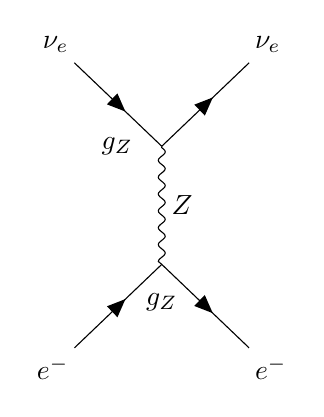
\begin{tikzpicture}
      \begin{feynman}
        \vertex (m1);
        \vertex [left=0.7em of m1] {$g_Z$};
        \vertex [above left=of m1] (i1) {$\nu_e$};
        \vertex [below=of m1] (m2);
        \vertex [below left=of m2] (i2) {$e^-$};
        \vertex [below=0.7em of m2] {$g_Z$};
        \vertex [above right=of m1] (f2) {$\nu_e$};
        \vertex [below right=of m2] (f1){$e^-$};
        \diagram*{
          (i1) -- [fermion] (m1) -- [fermion] (f2),
          (i2) -- [fermion] (m2),
          (m2) -- [fermion] (f1),
          (m1) -- [photon, edge label=$Z$] (m2)
        };
      \end{feynman}
    \end{tikzpicture}
\end{center}
\begin{center}
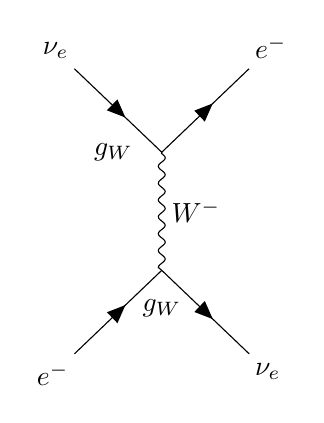
\begin{tikzpicture}
      \begin{feynman}
        \vertex (m1);
        \vertex [left=0.7em of m1] {$g_W$};
        \vertex [above left=of m1] (i1) {$\nu_e$};
        \vertex [below=of m1] (m2);
        \vertex [below left=of m2] (i2) {$e^-$};
        \vertex [below=0.7em of m2] {$g_W$};
        \vertex [above right=of m1] (f2) {$e^-$};
        \vertex [below right=of m2] (f1){$\nu_e$};
        \diagram*{
          (i1) -- [fermion] (m1) -- [fermion] (f2),
          (i2) -- [fermion] (m2),
          (m2) -- [fermion] (f1),
          (m1) -- [photon, edge label=$W^-$] (m2)
        };
      \end{feynman}
    \end{tikzpicture}
\end{center}
\item $\overline{\nu}_e e^-\rightarrow\overline{\nu}_e e^-$ Cannot have t-channel since lepton number will not be conserved at the vertices. We also needed to conserve charge.
\begin{center}
    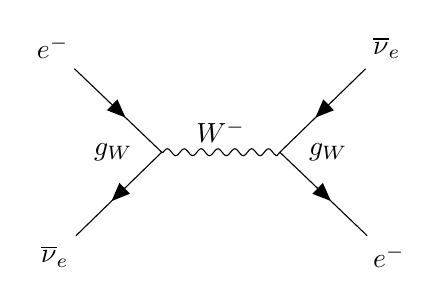
\begin{tikzpicture}
      \begin{feynman}
        \vertex (m1);
        \vertex [left=0.7em of m1] {$g_W$};
        \vertex [above left=of m1] (i1) {$e^-$};
        \vertex [below left=of m1] (i2) {$\overline{\nu}_e$};
        \vertex [right=of m1] (m2);
        \vertex [right=0.7em of m2] {$g_W$};
        \vertex [above right=of m2] (f2) {$\overline{\nu}_e$};
        \vertex [below right=of m2] (f1) {$e^-$};

        \diagram*{
          (i1) -- [fermion] (m1) -- [fermion] (i2),
          (f2) -- [fermion] (m2) -- [fermion] (f1),
          (m1) -- [photon, edge label=$W^-$] (m2)
        };
      \end{feynman}
    \end{tikzpicture}
\end{center}
\newpage
\item $\nu_\mu e^-\rightarrow\nu_\mu e^-$ Cannot have $W$ vector boson since charge has to be conserved. Cannot have s-channel since lepton number is not conserved.
\begin{center}
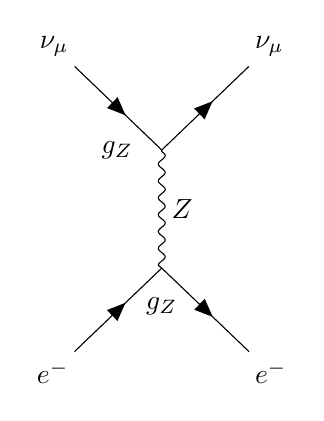
\begin{tikzpicture}
      \begin{feynman}
        \vertex (m1);
        \vertex [left=0.7em of m1] {$g_Z$};
        \vertex [above left=of m1] (i1) {$\nu_\mu$};
        \vertex [below=of m1] (m2);
        \vertex [below left=of m2] (i2) {$e^-$};
        \vertex [below=0.7em of m2] {$g_Z$};
        \vertex [above right=of m1] (f2) {$\nu_\mu$};
        \vertex [below right=of m2] (f1){$e^-$};
        \diagram*{
          (i1) -- [fermion] (m1) -- [fermion] (f2),
          (i2) -- [fermion] (m2),
          (m2) -- [fermion] (f1),
          (m1) -- [photon, edge label=$Z$] (m2)
        };
      \end{feynman}
    \end{tikzpicture}
\end{center}
\item $\overline{\nu}_\mu e^-\rightarrow\overline{\nu}_\mu e^-$ Cannot have charged current coupling across lepton generation.
\begin{center}
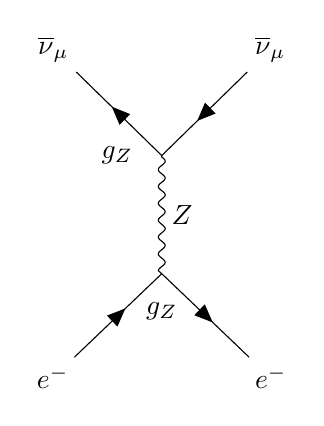
\begin{tikzpicture}
      \begin{feynman}
        \vertex (m1);
        \vertex [left=0.7em of m1] {$g_Z$};
        \vertex [above left=of m1] (i1) {$\overline{\nu}_\mu$};
        \vertex [below=of m1] (m2);
        \vertex [below left=of m2] (i2) {$e^-$};
        \vertex [below=0.7em of m2] {$g_Z$};
        \vertex [above right=of m1] (f2) {$\overline{\nu}_\mu$};
        \vertex [below right=of m2] (f1){$e^-$};
        \diagram*{
          (m1) -- [fermion] (i1),
          (f2)-- [fermion] (m1),
          (i2) -- [fermion] (m2),
          (m2) -- [fermion] (f1),
          (m1) -- [photon, edge label=$Z$] (m2)
        };
      \end{feynman}
    \end{tikzpicture}
\end{center}
\item $n\nu_e\rightarrow e^-p$ Flavour changing so charged current involves $W$.
\begin{center}
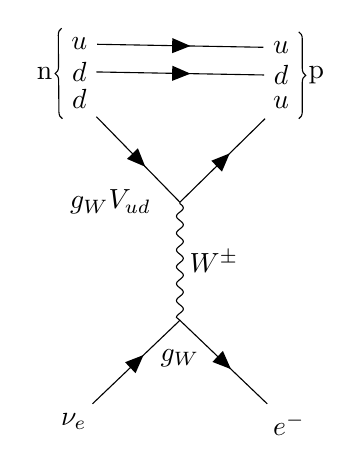
\begin{tikzpicture}
      \begin{feynman}
        \vertex (m1);
        \vertex [left=0.7em of m1] {$g_WV_{ud}$};
        \vertex [above left=of m1] (i1) {$d$};
        \vertex [above=1 em of i1] (si2) {$d$};
        \vertex [above=1 em of si2] (si1) {$u$};
        \vertex [below=of m1] (m2);
        \vertex [below left=of m2] (i2) {$\nu_e$};
        \vertex [below=0.7em of m2] {$g_W$};
        \vertex [above right=of m1] (f2) {$u$};
        \vertex [below right=of m2] (f1){$e^-$};
        \vertex [above=1 em of f2] (sf2) {$d$};
        \vertex [above=1 em of sf2] (sf1) {$u$};
        \diagram*{
          (i1) -- [fermion] (m1) -- [fermion] (f2),
          (i2) -- [fermion] (m2),
          (m2) -- [fermion] (f1),
          (m1) -- [photon, edge label=$W^\pm$] (m2),
          (si1) -- [fermion] (sf1),
          (si2) -- [fermion] (sf2)
        };
        \draw [decoration={brace}, decorate] (i1.south west) -- (si1.north west)
          node [pos=0.5, left] {n};
        \draw [decoration={brace}, decorate] (sf1.north east) -- (f2.south east)
          node [pos=0.5, right] {p};
      \end{feynman}
    \end{tikzpicture}
\end{center}
Here, both time ordering processes are considered.
\end{enumerate}
\end{ans}
\newpage
\begin{qns}[Weak force and conservation]
Consider each of the groups of processes given below. In each group, with the aid of Feynman diagrams using the Standard Model vertices, determine which processes are allowed and which are forbidden. By considering the strength of the forces involved, rank the processes in each group in order of expected rate.
\begin{center}
    \begin{tabular}{ccc}
        $\pi^0\rightarrow\gamma\gamma$ & $\pi^0\rightarrow\pi^-e^+\nu_e$ & $\pi^0\rightarrow\nu\overline{\nu}$ \\
       $e^+e^-\rightarrow\tau^+\tau^-$ & $\overline{\nu}_\mu+\tau^-\rightarrow\tau^-+\overline{\nu}_\mu$ & $\nu_\tau+p\rightarrow\tau^++n$ \\
       $B^0(\overline{b}d)\rightarrow D^-(\overline{c}d)\pi^+$ & $B^0\rightarrow\pi^+\pi^-$ & $B^0\rightarrow J/\psi~K^0$\\
       $D^0(c\overline{u})\rightarrow K^-\pi^+$ & $D^0\rightarrow\pi^+\pi^-$ & $D^0\rightarrow K^+\pi^-$\\
    \end{tabular}
\end{center}
\end{qns}
\begin{ans}\leavevmode
\begin{enumerate}
\item $\pi^0\rightarrow\gamma\gamma$ with $\pi^0$ ($u\overline{u}$)
   \begin{center}
    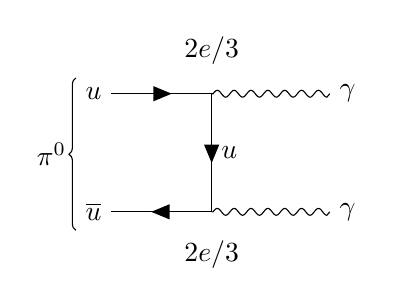
\begin{tikzpicture}
      \begin{feynman}
        \vertex (i1) {$u$};
        \vertex [below=of i1] (i2) {$\overline{u}$};
        \vertex [right=of i1] (m1);
        \vertex [above=0.7 em of m1] {$2e/3$};
        \vertex [right=of m1] (f1) {$\gamma$};
        \vertex [right=of i2] (m2);
        \vertex [below=0.7 em of m2] {$2e/3$};
        \vertex [right=of m2] (f2) {$\gamma$};

        \diagram* {
          (i1) -- [fermion] (m1),
          (m2) -- [fermion] (i2),
          (m1) -- [photon] (f1),
          (m2) -- [photon] (f2),

          (m1) -- [fermion, edge label=$u$] (m2);
        };
        \draw [decoration={brace}, decorate] (i2.south west) -- (i1.north west)
          node [pos=0.5, left] {$\pi^0$};
      \end{feynman}
    \end{tikzpicture}
  \end{center}
  This is a EM vertex with cross-section $\sigma\propto\frac{16}{81}e^4$ and it is allowed.\\[5pt]
  $\pi^0\rightarrow\pi^-e^+\nu_e$ with $\pi^0$ ($d\overline{d}$), $\pi^-$ ($d\overline{u}$)
      \begin{center}
        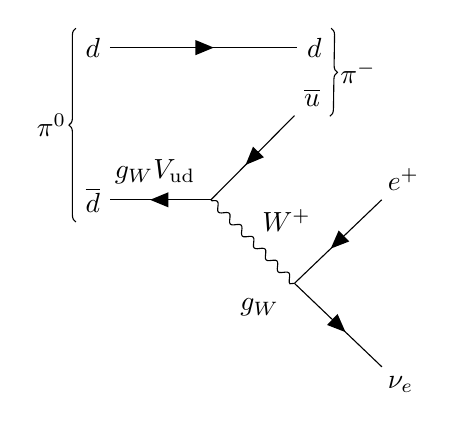
\begin{tikzpicture}
      \begin{feynman}
        \vertex (i1) {$\overline{d}$};
        \vertex [right=of i1] (m1);
        \vertex [above left=0.3 em of m1] {$g_WV_{\text{ud}}$};
        \vertex [above right=of m1] (f1) {$\overline{u}$};
        \vertex [below right=of m1] (m3);
        \vertex [below left=0.3 em of m3] {$g_W$};
        \vertex [above right=of m3] (f2) {$e^+$};
        \vertex [below right=of m3] (f3) {$\nu_e$};
         \vertex [above= 5.5 em of i1] (si1) {$d$};
        \vertex [right= 8 em of si1] (sf1) {$d$};
        \diagram* {
          (m1) -- [fermion] (i1),
          (si1) -- [fermion] (sf1),
          (f1) -- [fermion] (m1),
          (m1) -- [photon, edge label = $W^+$] (m3),
          (f2) -- [fermion] (m3),
          (m3) -- [fermion] (f3)
        };
        \draw [decoration={brace}, decorate] (i1.south west) -- (si1.north west)
          node [pos=0.5, left] {$\pi^0$};
        \draw [decoration={brace}, decorate] (sf1.north east) -- (f1.south east)
          node [pos=0.5, right] {$\pi^-$};
      \end{feynman}
    \end{tikzpicture}
    \end{center}
    Weak interaction plausible, but $m_{\pi^0}=134.98$ MeV/c$^2$, while $m_{\pi^-}=139.57$ MeV/c$^2>m_{\pi^0}$, so kinematically forbidden.\\[5pt]
    $\pi^0\rightarrow\nu\overline{\nu}$ with $\pi^0$ ($u\overline{u}$)
    \begin{center}
    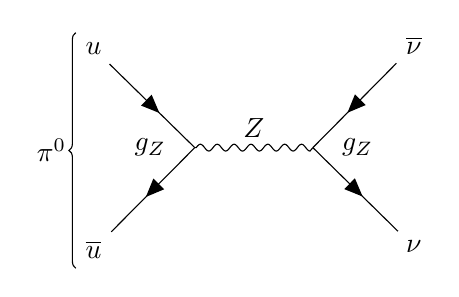
\begin{tikzpicture}
      \begin{feynman}
        \vertex (m1);
        \vertex [left=0.7em of m1] {$g_Z$};
        \vertex [above left=of m1] (i1) {$u$};
        \vertex [below left=of m1] (i2) {$\overline{u}$};
        \vertex [right=of m1] (m2);
        \vertex [right=0.7em of m2] {$g_Z$};
        \vertex [above right=of m2] (f2) {$\overline{\nu}$};
        \vertex [below right=of m2] (f1) {$\nu$};

        \diagram*{
          (i1) -- [fermion] (m1) -- [fermion] (i2),
          (f2) -- [fermion] (m2) -- [fermion] (f1),
          (m1) -- [photon, edge label=$Z$] (m2)
        };
        \draw [decoration={brace}, decorate] (i2.south west) -- (i1.north west)
          node [pos=0.5, left] {$\pi^0$};
      \end{feynman}
    \end{tikzpicture}
\end{center}
Weak interaction plausible with Feynman diagram as above. This is kinematically possible since $m_u>>m_\nu$. The cross-section is $\sigma\propto g_Z^4\propto\frac{e^4}{\sin^4\theta\cos^4\theta}$. But, $J_{\pi^0}=0$, and we have the two products travel in opposite directions in the frame of $\pi^0$. The neutrinos are fermions, each with spin-1/2. If the spin is along the momentum $\vec{p}$, we have a right-handed state. But right-handed neutrinos do not exist. The neutrino must be left-handed, with spin anti-parallel with $\vec{p}$, thus violating conservation of angular momentum. Hence, this reaction is forbidden.\\[5pt]
Only $\pi^0\rightarrow\gamma\gamma$ will occur.
\newpage
\item $e^+e^-\rightarrow\tau^+\tau^-$: EM or weak interactions possible. s-channel to conserve lepton number.
    \begin{center}
    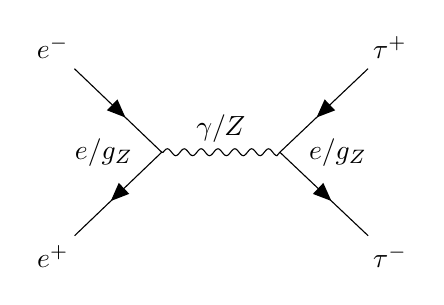
\begin{tikzpicture}
      \begin{feynman}
        \vertex (m1);
        \vertex [left=0.7em of m1] {$e/g_Z$};
        \vertex [above left=of m1] (i1) {$e^-$};
        \vertex [below left=of m1] (i2) {$e^+$};
        \vertex [right=of m1] (m2);
        \vertex [right=0.7em of m2] {$e/g_Z$};
        \vertex [above right=of m2] (f2) {$\tau^+$};
        \vertex [below right=of m2] (f1) {$\tau^-$};

        \diagram*{
          (i1) -- [fermion] (m1) -- [fermion] (i2),
          (f2) -- [fermion] (m2) -- [fermion] (f1),
          (m1) -- [photon, edge label=$\gamma/Z$] (m2)
        };
      \end{feynman}
    \end{tikzpicture}
\end{center}
$\overline{\nu}_\mu+\tau^-\rightarrow\overline{\nu}_\mu+\tau^-$: Weak interactions only. t-channel to conserve lepton number.
\begin{center}
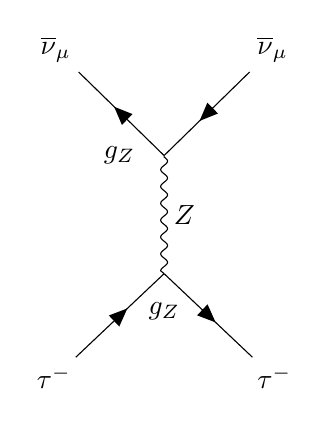
\begin{tikzpicture}
      \begin{feynman}
        \vertex (m1);
        \vertex [left=0.7em of m1] {$g_Z$};
        \vertex [above left=of m1] (i1) {$\overline{\nu}_\mu$};
        \vertex [below=of m1] (m2);
        \vertex [below left=of m2] (i2) {$\tau^-$};
        \vertex [below=0.7em of m2] {$g_Z$};
        \vertex [above right=of m1] (f2) {$\overline{\nu}_\mu$};
        \vertex [below right=of m2] (f1){$\tau^-$};
        \diagram*{
          (m1) -- [fermion] (i1),
          (f2)-- [fermion] (m1),
          (i2) -- [fermion] (m2),
          (m2) -- [fermion] (f1),
          (m1) -- [photon, edge label=$Z$] (m2)
        };
      \end{feynman}
    \end{tikzpicture}
\end{center}
$\nu_\tau+p\rightarrow\tau^++n$
      \begin{center}
        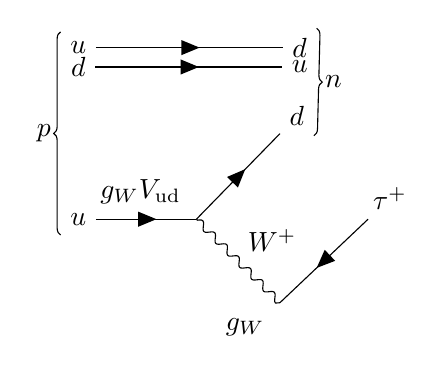
\begin{tikzpicture}
      \begin{feynman}
        \vertex (i1) {$u$};
        \vertex [right=of i1] (m1);
        \vertex [above left=0.3 em of m1] {$g_WV_{\text{ud}}$};
        \vertex [above right=of m1] (f1) {$d$};
        \vertex [below right=of m1] (m3);
        \vertex [below left=0.3 em of m3] {$g_W$};
        \vertex [above right=of m3] (f2) {$\tau^+$};
         \vertex [above= 5.5 em of i1] (si1) {$d$};
         \vertex [above= 0.7 em of si1] (si2) {$u$};
        \vertex [right= 8 em of si1] (sf1) {$u$};
        \vertex [right= 8 em of si2] (sf2) {$d$};
        \diagram* {
          (i1) -- [fermion] (m1),
          (si1) -- [fermion] (sf1),
          (si2) -- [fermion] (sf2),
          (m1) -- [fermion] (f1),
          (m1) -- [photon, edge label = $W^+$] (m3),
          (f2) -- [fermion] (m3)
        };
        \draw [decoration={brace}, decorate] (i1.south west) -- (si2.north west)
          node [pos=0.5, left] {$p$};
        \draw [decoration={brace}, decorate] (sf2.north east) -- (f1.south east)
          node [pos=0.5, right] {$n$};
      \end{feynman}
    \end{tikzpicture}
    \end{center}
    Lepton number is not conserved, so this reaction is forbidden.\\[5pt]
    The two allowed reactions with relative rates are $\Gamma(e^+e^-\rightarrow\tau^+\tau^-)>\Gamma(\overline{\nu}_\mu+\tau^-\rightarrow\tau^-+\overline{\nu}_\mu)$. This is because the former can happen with either $\gamma$ or $Z$ as the propagator.
\newpage
\item $B^0$ ($\overline{b}d$)$\rightarrow D^-$ ($\overline{c}d$)$\pi^+$($u\overline{d}$)
     \begin{center}
        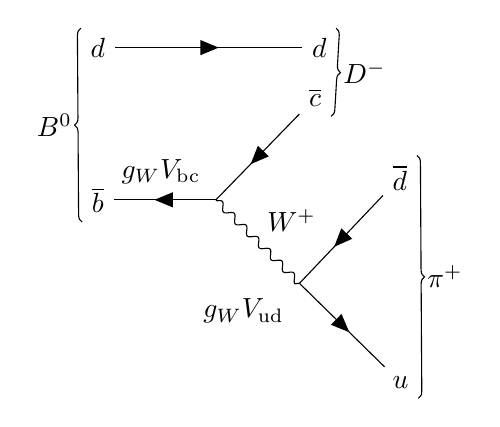
\begin{tikzpicture}
      \begin{feynman}
        \vertex (i1) {$\overline{b}$};
        \vertex [right=of i1] (m1);
        \vertex [above left=0.3 em of m1] {$g_WV_{\text{bc}}$};
        \vertex [above right=of m1] (f1) {$\overline{c}$};
        \vertex [below right=of m1] (m3);
        \vertex [below left=0.3 em of m3] {$g_WV_{\text{ud}}$};
        \vertex [above right=of m3] (f2) {$\overline{d}$};
        \vertex [below right=of m3] (f3) {$u$};
         \vertex [above= 5.5 em of i1] (si1) {$d$};
        \vertex [right= 8 em of si1] (sf1) {$d$};
        \diagram* {
          (m1) -- [fermion] (i1),
          (si1) -- [fermion] (sf1),
          (f1) -- [fermion] (m1),
          (m1) -- [photon, edge label = $W^+$] (m3),
          (f2) -- [fermion] (m3),
          (m3) -- [fermion] (f3)
        };
        \draw [decoration={brace}, decorate] (i1.south west) -- (si1.north west)
          node [pos=0.5, left] {$B^0$};
        \draw [decoration={brace}, decorate] (sf1.north east) -- (f1.south east)
          node [pos=0.5, right] {$D^-$};
           \draw [decoration={brace}, decorate] (f2.north east) -- (f3.south east)
          node [pos=0.5, right] {$\pi^+$};
      \end{feynman}
    \end{tikzpicture}
    \end{center}
    Cabibbo allowed. The masses are $m_{B^0}=5279.5$ MeV/c$^2$, $m_{D^-}=1869.3$ MeV/c$^2$, $m_{\pi^+}=$139.6 MeV/c$^2$, so kinematically allowed.\\[5pt]
    $B^0$ ($\overline{b}d$)$\rightarrow \pi^-$ ($\overline{u}d$)$\pi^+$ ($u\overline{d}$)
     \begin{center}
        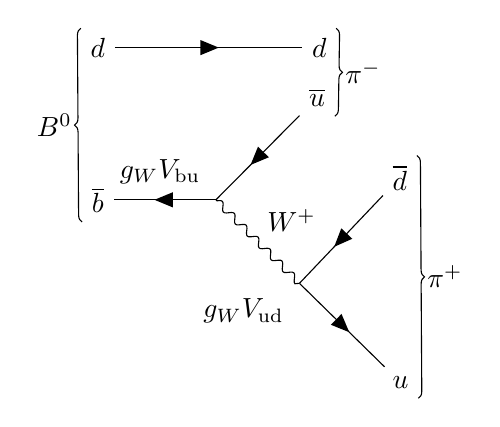
\begin{tikzpicture}
      \begin{feynman}
        \vertex (i1) {$\overline{b}$};
        \vertex [right=of i1] (m1);
        \vertex [above left=0.3 em of m1] {$g_WV_{\text{bu}}$};
        \vertex [above right=of m1] (f1) {$\overline{u}$};
        \vertex [below right=of m1] (m3);
        \vertex [below left=0.3 em of m3] {$g_WV_{\text{ud}}$};
        \vertex [above right=of m3] (f2) {$\overline{d}$};
        \vertex [below right=of m3] (f3) {$u$};
         \vertex [above= 5.5 em of i1] (si1) {$d$};
        \vertex [right= 8 em of si1] (sf1) {$d$};
        \diagram* {
          (m1) -- [fermion] (i1),
          (si1) -- [fermion] (sf1),
          (f1) -- [fermion] (m1),
          (m1) -- [photon, edge label = $W^+$] (m3),
          (f2) -- [fermion] (m3),
          (m3) -- [fermion] (f3)
        };
        \draw [decoration={brace}, decorate] (i1.south west) -- (si1.north west)
          node [pos=0.5, left] {$B^0$};
        \draw [decoration={brace}, decorate] (sf1.north east) -- (f1.south east)
          node [pos=0.5, right] {$\pi^-$};
           \draw [decoration={brace}, decorate] (f2.north east) -- (f3.south east)
          node [pos=0.5, right] {$\pi^+$};
      \end{feynman}
    \end{tikzpicture}
    \end{center}
    Doubly Cabibbo suppressed. The masses are $m_{B^0}=5279.5$ MeV/c$^2$ and $m_{\pi^+}=$139.6 MeV/c$^2$, so kinematically allowed.\\[5pt]
    $B^0$ ($\overline{b}d$)$\rightarrow$ J/$\psi$ (c$\overline{c}$)$K^0$ ($d\overline{s}$)
            \begin{center}
        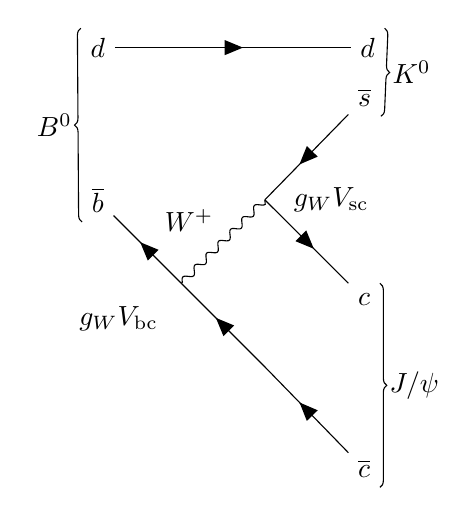
\begin{tikzpicture}
      \begin{feynman}
        \vertex (i1) {$\overline{b}$};
        \vertex [below right=of i1] (m1);
        \vertex [below left=0.7 em of m1] {$g_WV_{\text{bc}}$};
        \vertex [above right=of m1] (m3);
        \vertex [above right=of m3] (f1) {$\overline{s}$};
        \vertex [right=0.7 em of m3] {$g_WV_{\text{sc}}$};
        \vertex [below right=of m3] (f2) {$c$};
        \vertex [below right=of m1] (m4);
        \vertex [below right=of m4] (f3){$\overline{c}$};
         \vertex [above= 5.5 em of i1] (si1) {$d$};
        \vertex [right= 9.75 em of si1] (sf1) {$d$};
        \diagram* {
          (f3)--[fermion](m4) -- [fermion] (m1)--[fermion](i1),
          (si1) -- [fermion] (sf1),
          (m1) -- [photon, edge label = $W^+$] (m3),
          (m3) -- [fermion] (f2),
          (f1) -- [fermion] (m3)
        };
        \draw [decoration={brace}, decorate] (i1.south west) -- (si1.north west)
          node [pos=0.5, left] {$B^0$};
        \draw [decoration={brace}, decorate] (sf1.north east) -- (f1.south east)
          node [pos=0.5, right] {$K^0$};
           \draw [decoration={brace}, decorate] (f2.north east) -- (f3.south east)
          node [pos=0.5, right] {$J/\psi$};
      \end{feynman}
    \end{tikzpicture}
    \end{center}
    Singly Cabibbo suppressed. The masses are $m_{B^0}=5279.5$ MeV/c$^2$, $m_{J/\psi}=3096.9$ MeV/c$^2$ and $m_{K^0}=497.6$ MeV/c$^2$, so kinematically allowed.\\[5pt]
    Their relative rates are determined by the extent of Cabibbo suppression.
    \newpage
\item $D^0$ ($c\overline{u}$)$\rightarrow$ $K^-$ (s$\overline{u}$) $\pi^+$ (u$\overline{d}$)
  \begin{center}
        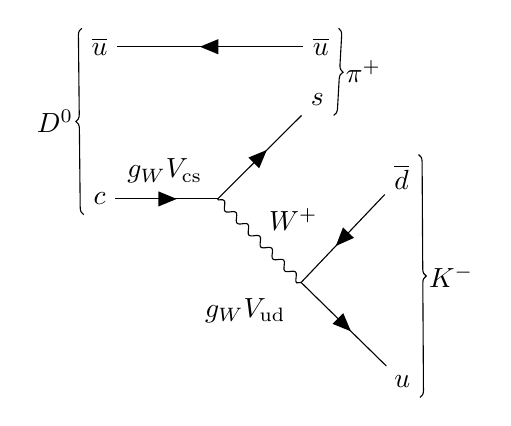
\begin{tikzpicture}
      \begin{feynman}
        \vertex (i1) {$c$};
        \vertex [right=of i1] (m1);
        \vertex [above left=0.3 em of m1] {$g_WV_{\text{cs}}$};
        \vertex [above right=of m1] (f1) {$s$};
        \vertex [below right=of m1] (m3);
        \vertex [below left=0.3 em of m3] {$g_WV_{\text{ud}}$};
        \vertex [above right=of m3] (f2) {$\overline{d}$};
        \vertex [below right=of m3] (f3) {$u$};
         \vertex [above= 5.5 em of i1] (si1) {$\overline{u}$};
        \vertex [right= 8 em of si1] (sf1) {$\overline{u}$};
        \diagram* {
          (i1) -- [fermion] (m1),
          (sf1) -- [fermion] (si1),
          (m1) -- [fermion] (f1),
          (m1) -- [photon, edge label = $W^+$] (m3),
          (f2) -- [fermion] (m3),
          (m3) -- [fermion] (f3)
        };
        \draw [decoration={brace}, decorate] (i1.south west) -- (si1.north west)
          node [pos=0.5, left] {$D^0$};
        \draw [decoration={brace}, decorate] (sf1.north east) -- (f1.south east)
          node [pos=0.5, right] {$\pi^+$};
           \draw [decoration={brace}, decorate] (f2.north east) -- (f3.south east)
          node [pos=0.5, right] {$K^-$};
      \end{feynman}
    \end{tikzpicture}
    \end{center}
    Cabibbo allowed. The masses are $m_{D^0}=1864.8$ MeV/c$^2$, $m_{K^-}=493.7$ MeV/c$^2$, $m_{\pi^+}=139.6$ MeV/c$^2$, so it is kinematically allowed.

    $D^0$ ($c\overline{u}$)$\rightarrow$ $\pi^+$ (u$\overline{d}$) $\pi^-$ (d$\overline{u}$)
  \begin{center}
        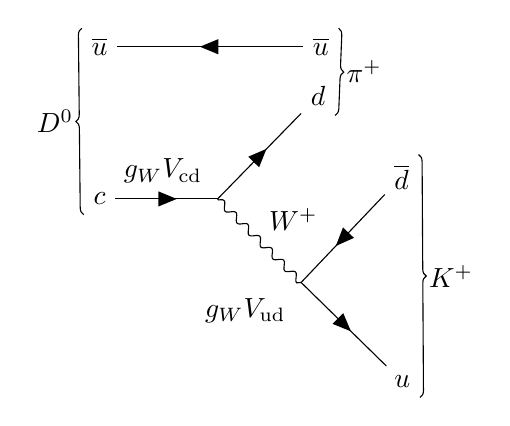
\begin{tikzpicture}
      \begin{feynman}
        \vertex (i1) {$c$};
        \vertex [right=of i1] (m1);
        \vertex [above left=0.3 em of m1] {$g_WV_{\text{cd}}$};
        \vertex [above right=of m1] (f1) {$d$};
        \vertex [below right=of m1] (m3);
        \vertex [below left=0.3 em of m3] {$g_WV_{\text{ud}}$};
        \vertex [above right=of m3] (f2) {$\overline{d}$};
        \vertex [below right=of m3] (f3) {$u$};
         \vertex [above= 5.5 em of i1] (si1) {$\overline{u}$};
        \vertex [right= 8 em of si1] (sf1) {$\overline{u}$};
        \diagram* {
          (i1) -- [fermion] (m1),
          (sf1) -- [fermion] (si1),
          (m1) -- [fermion] (f1),
          (m1) -- [photon, edge label = $W^+$] (m3),
          (f2) -- [fermion] (m3),
          (m3) -- [fermion] (f3)
        };
        \draw [decoration={brace}, decorate] (i1.south west) -- (si1.north west)
          node [pos=0.5, left] {$D^0$};
        \draw [decoration={brace}, decorate] (sf1.north east) -- (f1.south east)
          node [pos=0.5, right] {$\pi^+$};
           \draw [decoration={brace}, decorate] (f2.north east) -- (f3.south east)
          node [pos=0.5, right] {$K^+$};
      \end{feynman}
    \end{tikzpicture}
    \end{center}
Kinematically allowed, but singly Cabibbo suppressed.\\[5pt]
$D^0$ ($c\overline{u}$)$\rightarrow$ $\pi^-$ (d$\overline{u}$) $K^+$ (u$\overline{s}$)
  \begin{center}
        \begin{tikzpicture}
      \begin{feynman}
        \vertex (i1) {$c$};
        \vertex [right=of i1] (m1);
        \vertex [above left=0.3 em of m1] {$g_WV_{\text{cd}}$};
        \vertex [above right=of m1] (f1) {$d$};
        \vertex [below right=of m1] (m3);
        \vertex [below left=0.3 em of m3] {$g_WV_{\text{us}}$};
        \vertex [above right=of m3] (f2) {$\overline{s}$};
        \vertex [below right=of m3] (f3) {$u$};
         \vertex [above= 5.5 em of i1] (si1) {$\overline{u}$};
        \vertex [right= 8 em of si1] (sf1) {$\overline{u}$};
        \diagram* {
          (i1) -- [fermion] (m1),
          (sf1) -- [fermion] (si1),
          (m1) -- [fermion] (f1),
          (m1) -- [photon, edge label = $W^+$] (m3),
          (f2) -- [fermion] (m3),
          (m3) -- [fermion] (f3)
        };
        \draw [decoration={brace}, decorate] (i1.south west) -- (si1.north west)
          node [pos=0.5, left] {$D^0$};
        \draw [decoration={brace}, decorate] (sf1.north east) -- (f1.south east)
          node [pos=0.5, right] {$\pi^-$};
           \draw [decoration={brace}, decorate] (f2.north east) -- (f3.south east)
          node [pos=0.5, right] {$K^+$};
      \end{feynman}
    \end{tikzpicture}
    \end{center}
Kinematically allowed, but doubly Cabibbo suppressed.\\[5pt]
Their relative rates are determined by the extent of Cabibbo suppression.
\end{enumerate}
\end{ans}
\newpage
\subsection*{Neutrino oscillations}
\begin{qns}[$\nu$ oscillations]\leavevmode
\begin{enumerate}[label=(\alph*)]
    \item Show that if there are two neutrino mass eigenstates $\nu_2$ and $\nu_3$ with masses $m_2$ and $m_3$ and energies $E_2$ and $E_3$, mixed so that
    $$\nu_\mu=\nu_2\cos\theta+\nu_3\sin\theta$$
    $$\nu_\tau=-\nu_2\sin\theta+\nu_3\cos\theta$$
    then the number of muon neutrinos observed at a distance $L$ from the muon source is
    $$|\nu_\mu(L)|^2=|\nu_\mu(L=0)|^2\times\bigg[1-\sin^2(2\theta)\sin^2\bigg\{\bigg(\frac{E_3-E_2}{2\hbar}\bigg)\frac{L}{c}\bigg\}\bigg]$$
    \item If $m_2$ and $m_3$ are very much less than the neutrino momentum, $p$, show that
    $$|\nu_\mu(L)|^2\approx|\nu_\mu(L=0)|^2\times\bigg[1-\sin^2(2\theta)\sin^2\bigg\{A\bigg(\frac{(m_2^2-m_3^2)L}{p}\bigg)\bigg\}\bigg]$$
    where $A$ is a constant.
    \item In 2005 the MINOS experiment started to study neutrino oscillations by pointing a beam of 1-5 GeV/c muon neutrinos from Fermilab, Illinois, at the 5400 ton MINOS far dectector in the SOUDAN mine in Minnesota, 730 km away. The experiment aimed to make a precise measurement of $m^2_3-m_2^2$.\\[5pt] Sketch the expected energy spectrum of muon neutrinos at the MINOS far detector if $\sin^2(2\theta)=0.90$ and $m_3^2-m_2^2=2.5\times10^{-3}$ (eV/c$^2$)$^2$. Assume that the energy spectum of neutrinos produced by the beam at Fermilab is of uniform intensity in the range 1-5 GeV and zero elsewhere (i.e. a top-hat function).
    \item If muon neutrinos oscillate into tau neutrinos, will any $\tau$ leptons (produced by charged current interactions) be observed in the MINOS far detector?\\[5pt]
    Hint: You may find the result of qu.21 useful.
\end{enumerate}
[$A =$ 1.27 s$^{−1}$ if $m_2$ and $m_3$ are measured in eV/c$^2$, $p$ in GeV/c and $L$ in km. The mass of the $\tau^-$ is 1.777 GeV/c$^2$.]]
\end{qns}
\begin{ans}\leavevmode
\begin{enumerate}[label=(\alph*)]
\item At $t=0$, $L=0$, we observe purely muons, i.e. $\psi(t=0)=\nu_\mu=\nu_2\cos\theta+\nu_3\sin\theta$. Inverting the state matrix:
$$\begin{pmatrix}\nu_\mu\\\nu_\tau\\\end{pmatrix}=\begin{pmatrix}\cos\theta&\sin\theta\\-\sin\theta&\cos\theta\\\end{pmatrix}\begin{pmatrix}\nu_2\\\nu_3\\\end{pmatrix}\implies\begin{pmatrix}\nu_2\\\nu_3\\\end{pmatrix}=\begin{pmatrix}\cos\theta&-\sin\theta\\\sin\theta&\cos\theta\\\end{pmatrix}\begin{pmatrix}\nu_\mu\\\nu_\tau\\\end{pmatrix}$$
The wavefunction is thus
\begin{align}
\psi(t)&=\nu_2e^{-iE_2t/\hbar}\cos\theta+\nu_3e^{-iE_3t/\hbar}\sin\theta\nonumber\\&=(\nu_\mu\cos\theta-\nu_\tau\sin\theta)e^{-iE_2t/\hbar}\cos\theta+(\nu_\mu\sin\theta+\nu_\tau\cos\theta)e^{-iE_3t/\hbar}\sin\theta\nonumber\\&=\nu_\mu(\cos^2\theta~e^{-iE_2t/\hbar}+\sin^2\theta~e^{-iE_3t/\hbar})+\nu_\tau\sin\theta\cos\theta(e^{-iE_3t/\hbar}-e^{-iE_2t/\hbar})\nonumber
\end{align}
The probability of observing a tau neutrino is
\begin{align}
    |c_\tau|^2&=\sin^2\theta\cos^2\theta\bigg|e^{-iE_3t/\hbar}-e^{-iE_2t/\hbar}\bigg|^2\nonumber\\&=\frac{1}{4}\sin^22\theta(e^{iE_3t/\hbar}-e^{iE_2t/\hbar})(e^{-iE_3t/\hbar}-e^{-iE_2t/\hbar})\nonumber\\&=\frac{1}{4}\sin^22\theta(2-e^{i(E_2-E_3)t/\hbar}-e^{-i(E_3-E_2)t/\hbar})\nonumber\\&=\frac{1}{4}\sin^22\theta\frac{(e^{i(E_2-E_3)t/2\hbar}-e^{-i(E_2-E_3)t/2\hbar})^2}{i^2}\nonumber\\&=\frac{1}{4}\sin^22\theta~4\sin^2\frac{(E_3-E_2)t}{2\hbar}\nonumber
\end{align}
The number of muon neutrinos at a distance $L$ is
$$\nu_\mu(L)=\nu_\mu(L=0)(1-p(\nu_\tau))\implies|\nu_\mu(L)|^2=|\nu_\mu(L=0)|^2\bigg(1-\sin^22\theta\sin^2\frac{(E_3-E_2)}{2\hbar}\frac{L}{c}\bigg)$$
\item Assuming $m_2,m_3<<p$, we have
$$E_i=\sqrt{p^2+m_i^2}=p\sqrt{1+\frac{m_i^2}{p^2}}\approx p\bigg(1+\frac{m_i^2}{2p^2}\bigg)\implies E_3-E_2=\frac{m_3^2-m_2^2}{2p}$$
Hence, we approximate
$$|\nu_\mu(L)|^2\approx|\nu_\mu(L=0)|^2\bigg[1-\sin^22\theta\sin^2\frac{m_3^2-m_2^2}{4p\hbar}\frac{L}{c}\bigg]$$
We read off $A=-\frac{1}{4\hbar c}=-1.27$ GeV$^{-1}$fm$^{-1}=-1.27\times10^6$ eV$^{-1}$m$^{-1}$.
\item Plug the values into the equation:
$$\frac{|\nu_\mu(L)|^2}{|\nu_\mu(0)|^2}\approx 1-0.9\sin^2\frac{(2.5\times10^{-3}(\text{eV/c}^2)^2(1.27\times10^6\text{eV}^{-1}\text{m}^{-1})(730\times10^3\text{m})}{E}=1-0.9\sin^2\frac{2.32}{E}$$
where $E$ is in GeV.
\begin{center}
\begin{tikzpicture}
      \draw[->] (0,0) -- (6,0) node[right] {$E/$GeV};
      \draw[->] (0,0) -- (0,4) node[left] {$|\nu_\mu(L)|^2/|\nu_\mu(0)|^2$};
      \draw[domain=1:5,smooth,variable=\x,black] plot ({\x},{3*(1-0.9*(sin(deg(2.32/\x))^2)});
      \draw (1,0) node[below]{1};
      \draw (5,0) node[below]{5};
\end{tikzpicture}
\end{center}
\item From Q21b, $E_{\nu,\text{min}}=3.47$ GeV. A smaller energy range 3.47 to 5 GeV is possible for neutrino oscillation. A few tau leptons ($n\nu_\tau\rightarrow p\tau^-$) can be observed in the MINOS far detector.
\end{enumerate}
\end{ans}
\newpage
\section{Example Sheet 4}
\subsection*{Basic nuclear properties}
\begin{qns}[SEMF]
The Semi-Empirical mass formula (SEMF) for nuclear masses may be written in the form
$$M(A,Z)=Zm_p+(A-Z)m_n-a_VA+a_SA^{2/3}+a_C\frac{Z^2}{A^{1/3}}+a_A\frac{(A-2Z)^2}{A}+\delta (A,Z)$$
where $m_p$ and $m_n$ are the masses of the proton and neutron respectively. Fitted values for the coefficients are given at the end of the question.
\begin{enumerate}[label=(\alph*)]
    \item Explain the physical significance and functional form of the various terms.
    \item  Treating the nucleus as a sphere of uniform charge density, show that the constant
    $$a_C=\frac{3e^2}{20\pi\varepsilon_0R_0}=0.72 \text{ MeV}$$
    \item By reference to the SEMF explain in physical terms why nuclear fission and fusion are possible.
    \item Use the Semi-Empirical mass formula to predict that the value of $Z$ of the most stable isobar of mass number $A$ is
    $$Z=\frac{m_n-m_p+4a_A}{2a_cA^{-1/3}+8a_A/A}$$
    Predict the $Z$ for the most stable nuclei with $A = 101$ and $A = 191$. Compare with nuclear data, which you can find on the web (e.g. \url{http://www.nndc.bnl.gov/chart/}). Predict the most stable super-heavy nucleus with mass number 300.
    \item  Show that the effect of gravitational binding in the nucleus may be accounted for by adding a term $−a_GA^{5/3}$ to the SEMF (neglecting the proton-neutron mass difference). Show that $a_G$ is given by
    $$a_G=\frac{3Gm_n^2}{5E_0}\approx 5.8\times10^{-37}\text{ MeV}$$
    Use the SEMF, so modified, to estimate that the lightest `nucleus' consisting entirely of neutrons (i.e. a neutron star) has a mass approximately 10\% that of the sun. Amazingly enough, this reckless extrapolation over more than 50 orders of magnitude turns out to give more or less the right answer!\\[5pt]
    {Take the mass of the Sun to be $2\times10^{30}$ kg.}
\end{enumerate}
[Use the following data: $m_p=938.3$ MeV, $m_n=939.6$ MeV, $m_e=0.511$ MeV, $a_V=15.8$ MeV, $a_S=18.0$ MeV, $a_A=23.5$ MeV. Nuclear radius $R=R_0A^{1/3}$ with $R_0=1.2$ fm.]
\end{qns}
\begin{ans}\leavevmode
\begin{enumerate}[label=(\alph*)]
\item The terms are:
\begin{itemize}
    \item $Zm_p+(A-Z)m_n$ is the sum of proton and neutron mass. The remaining terms are binding energies.
    \item $a_VA$ is a volume term. The more nucleons present, the larger the volume $V$, the higher the binding energy $B$, i.e. $V\propto A\propto R^3,~B\propto V$
    \item $a_SA^{2/3}$ is a surface term. The surface nucleons are not as strongly bound. The larger the surface area $\mathcal{A}$, the smaller $B$ is, i.e. $\mathcal{A}\propto R^2\propto A^{2/3}$ with $B\propto-\mathcal{A}$
    \item $a_CZ^2/A^{1/3}$ is the repulsive electromagnetic forces between protons, which decreases the binding energy. It is $\propto Z^2/R\propto Z^2/A^{1/3}$, i.e. electrostatic potential energy
    \item $a_A(A-2Z)^2/A$ is the asymmetry term. Nuclei with $N\sim Z$ ($A=2Z$) tend to be stable. This term decreases the binding energy. It is less the further we move away from $N=2$. This term scales as $1/A$ with the levels being more closely spaced as $A$ increases. So for large $A$, this term's contribution is small.
    \item $\delta (A,Z)$ is the pairing term. If $Z$ and $N$ are even, the nucleus is particularly stable. This term increases the binding energy and depends like $A^{-3/4}$, i.e. effect decreases for heavier nuclei. $\delta (A,Z)<0$ for $Z,N$ even; $\delta (A,Z)>0$ for $Z, N$ odd; $\delta(A,Z)=0$ for even-odd nuclei. 
\end{itemize}
\item Consider a sphere of uniform charge density $\rho=3Ze/4\pi R^3$. The shell at $r$ feels $-\frac{Zer^3}{R^3}\frac{1}{4\pi\varepsilon_0r}$ due to the charge enclosed by a spherical volume of radius $r$. Due to spherical symmetry, the total energy of the sphere is done by summing the contributions of individual successive spherical shells, $\int \Phi_{\text{shell}} dQ$. But we have
$$\frac{dQ}{4\pi r^2dr}=\frac{Ze\rho}{(4/3)\pi R^3}\implies dQ=\frac{3Zer^2}{R^3}dr$$
We have
$$U_E=-\int_0^R\frac{Zer^3}{R^3}\frac{3Zer^2}{R^3}\frac{1}{4\pi\varepsilon_0r}dr=-\int_0^R\frac{Z^2e^2}{R^6}\frac{3}{4\pi\varepsilon_0}r^4dr=-\frac{Z^2e^2}{R^6}\frac{3}{4\pi\varepsilon_0}\frac{R^5}{5}=-\frac{3Z^2e^2}{20\pi\varepsilon_0R}$$
But $R=R_0 A^{1/3}$, where $R_0=1.2$ fm, hence comparing with $a_CZ^2/A^{1/3}$, we have
$$a_C=\frac{3e^2}{20R_0\pi\varepsilon_0}=\frac{3(1.6\times10^{-19}\text{C})^2}{20(1.2\times10^{-15}\text{m})\pi(8.85\times10^{-12}\text{F/m})}=0.72~\text{MeV}$$
\item In nuclear fission and fusion, the total number of nucleons is the same, so the difference in binding energy dictates whether energy is released in the process. The SEMF expression for binding energy has a maximum at Fe, i.e. nuclei with $Z$ smaller than Fe undergoes fusion to increase binding energy, whereas nuclei with $Z$ larger than Fe undergoes fission.
\item The nuclei is most stable when $M(A,Z)$ is minimized with respect to $Z$ at constant $A$, i.e. $(\frac{\partial M}{\partial Z})_A=0$, i.e.
$$0=m_p-m_n+\frac{2a_C}{A^{1/3}}Z-2a_n\frac{(A-2Z)2}{A}=m_p-m_n-4a_A+Z\bigg(\frac{2a_C}{A^{1/3}}+\frac{8a_A}{A}\bigg)\implies Z=\frac{m_n-m_p+4a_A}{(2a_c/A^{1/3})+(8a_A/A)}$$
where $m_n=939.6$ MeV, $m_p=938.3$ MeV, $a_A=23.5$ MeV, $a_C=0.72$ MeV, $a_A=23.5$ MeV. Plugging in $A=101$, 191, 300 respectively gives $\approx 44,$ 77, 113 (i.e. Ru, Ir for the first two).
\item Gravitational force is a central potential (spherical symmetry), hence we can use the successive spherical shell method. The gravitational potential energy on an element is $GM_{\text{enclosed}} dm/r$. But, 
$$\frac{M_{\text{encl}}}{r^3}=\frac{Am_n}{R^3},\quad\frac{dm}{4\pi r^2dr}=\frac{Am_n}{(4/3)\pi R^3}$$
This gives the total self-gravitational potential energy to be
$$U_G=\int_0^R\frac{G}{r}\frac{Am_nr^3}{R^3}\frac{3Am_n}{R^3}r^2dr=\frac{3GA^2m_n^2}{R^6}\int_0^Rr^4dr=\frac{3GA^2}{5R}m_n^2=\frac{3Gm_n^2}{5R_0}A^{5/3}\propto A^{5/3}$$
where $R=R_0A^{1/3}$. The constant is
$$a_G=\frac{3Gm_n^2}{5R_0}=\frac{3(6.67\times10^{-11}\text{N m}^2\text{kg}^{-2})(939.6\times10^6)\text{eV}(1.6\times10^{-19}\text{J/eV}}{5(1.2\times10^{-15}\text{m})(3\times10^8\text{m/s})^4}=5.8\times10^{-37}~\text{MeV}$$
This is stable if $Am_n>B>0$, where $B=a_VA-a_SA^{2/3}-a_AA+a_GA^{5/3}$. Consider a neutron star, $A=N$, $Z=0$, then
$$0=a_VN-a_SN^{2/3}-a_AN+a_GN^{5/3}\implies N=\bigg(\frac{a_A-a_V}{a_G}\bigg)^{3/2}=\bigg(\frac{(23.5-15.8)~\text{MeV}}{5.8\times10^{-37}~\text{MeV}}\bigg)^{3/2}=4.84\times10^{55}$$
where we assume $N$ is large, and the final numerical result is consistent with the assumption.
\end{enumerate}
\end{ans}
\newpage
\begin{qns}[Fermi Gas model]
We can predict the form of the asymmetry term, and estimate its magnitude, using the Fermi Gas model. This involves treating the $N$ neutrons and $Z$ protons as free fermions of mass $m$ moving in a box of volume $V=\frac{4}{3}\pi R_0^3A$. The model therefore only accounts for the kinetic energy of the nucleons, and not their potential energy.\\[5pt]
A standard calculation, which you have done before (at least for a cubic box), gives the density of states for each species (including spin degeneracy) as
$$g(E)=BAE^{1/2}\text{ where } B=\frac{4\sqrt{2}m^{3/2}R_0^3}{3\pi\hbar^3}$$
You need not prove this unless you want to practice. Show that the Fermi energy for the neutrons is
$$E_F=\bigg(\frac{3N}{2BA}\bigg)^{2/3}$$
Calculate the Fermi energy $\overline{E}_F$ and the corresponding nucleon momentum for the symmetric case $N=Z=0.5 A$.\\[5pt]
Show that the total kinetic energy of the nucleons is given by
$$\frac{3}{5}\bigg(\frac{3}{2BA}\bigg)^{2/3}(N^{5/3}+Z^{5/3})$$
Expand about the symmetric point $N=Z=\frac{1}{2}A$ by writing $N=\frac{1}{2}A(1+\alpha)$ and $Z=\frac{1}{2}A(1-\alpha)$ to show that the asymmetry energy has the form:
$$a_A\frac{(N-Z)^2}{A}\text{ where }a_A=\frac{1}{3}\overline{E}_F$$
Note that this underestimates the empirical value, because this model does not take account of the potential energy, which also depends on $(N − Z)$.\\[5pt]
One contribution to the pairing energy can also be estimated from this model, reflecting the stepwise increase of the kinetic energy resulting from the exclusion principle. This would be expected to be approximately equal to the energy spacing of levels at the Fermi level, i.e. $1/g(E_F)$. Show that this is, for the $N = Z =\frac{1}{2}A$ case:
$$\frac{4\overline{E}_F}{3A}$$
Evaluate and compare with the fitted value in the SEMF for a typical value of A. Note that the Fermi Gas model again gives an underestimate because it does not take account of the additional potential energy arising from the spatial overlap of two nucleons in the same energy level.
\end{qns}
\begin{ans}
For $N$ neutrons, the Fermi sphere is filled up to energy $E_F$:
$$N=\int_0^{E_F}g(E)dE=BA\int_0^{E_F}E^{1/2}dE=BAE_F^{3/2}\frac{2}{3}\implies E_F=\bigg(\frac{3N}{2BA}\bigg)^{2/3}$$
For the symmetric case $N=Z=A/2$ and with $R_0=1.2$ fm:
$$\overline{E}_F=\bigg(\frac{3}{4B}\bigg)^{2/3}=\bigg(\frac{3}{4}\frac{3\pi}{4\sqrt{2}}\frac{(6.626\times10^{-34}/2\pi)^3}{(1.66\times10^{-27})^{3/2}(1.2\times10^{-15})^3}\bigg)^{2/3}=33.4~\text{MeV}$$
The corresponding momentum is $p=\sqrt{2mE_F}=2\sqrt{(33.4)(939.6)}=250$ MeV/c. The total kinetic energy of $N$ neutrons is
$$E_k=\int_0^{E_F}Eg(E)dE=BA\int_0^{E_F}E^{3/2}dE=\frac{2BA}{5}E_F^{5/2}=\frac{2}{5}BA\bigg(\frac{3N}{2BA}\bigg)^{5/3}=\frac{3}{5}\bigg(\frac{3}{2BA}\bigg)^{2/3}N^{5/3}$$
Similarly, for $Z$ protons, the total kinetic energy is $\frac{3}{5}(\frac{3}{2BA})^{2/3}Z^{5/3}$. The total kinetic energy of the nucleons is the sum of both.\\[5pt]
Expand about $N=Z=A/2$,
$$N^{5/3}\approx\bigg(\frac{1}{2}A\bigg)^{5/3}\bigg(1+\frac{5}{3}\alpha+\frac{5}{3}\frac{2}{3}\frac{1}{2}\alpha^2+\dots\bigg),\quad Z^{5/3}\approx\bigg(\frac{1}{2}A\bigg)^{5/3}\bigg(1-\frac{5}{3}\alpha+\frac{5}{3}\frac{2}{3}\frac{1}{2}\alpha^2+\dots\bigg)$$
It follows that, the total kinetic energy is
$$\frac{3}{5}\bigg(\frac{3}{2BA}\bigg)^{2/3}\bigg(\frac{1}{2}A\bigg)^{5/3}\bigg(2+\frac{10}{9}\bigg(\frac{N-Z}{A}\bigg)^2\bigg)$$
where $N-Z=A\alpha$. Identify the asymmetric part to be $a_A(N-Z)^2/A$, hence giving 
$$a_A=\frac{2}{3}\bigg(\frac{3}{2BA}\bigg)^{2/3}\frac{1}{A}\bigg(\frac{A}{2}\bigg)^{5/3}=\frac{1}{3(2)^{2/3}}\bigg(\frac{3}{2B}\bigg)^{2/3}=\frac{\overline{E}_F}{3}\approx 11~\text{MeV}$$
For the symmetric case, $1/g(E_F)$ is
$$\frac{1}{g(E_F)}=\frac{1}{BAE^{1/2}}=\frac{1}{BA}\bigg(\frac{4B}{3}\bigg)^{1/3}=\frac{4\overline{E}_F}{3A}$$
where $\overline{E}_F=(3/4B)^{2/3}$.
\end{ans}
\begin{qns}[Nuclear size]
A spherically symmetric nucleus has a radial charge density $\rho(r)$ which is normalised such that $\int\rho(r)d^3\mathbf{r}=1$. Show that in this case the form factor is given by:
$$F(q^2)=\frac{4\pi}{q}\int_0^\infty r\sin qr~\rho(r)dr$$
which can then be approximated by
$$F(q^2)\approx 1-\frac{1}{6}q^2\overline{R^2}+\dots$$
in natural units, where $\overline{R^2}$ is the mean square radius of the charge distribution. When elastic scattering of 200 MeV electrons from a gold foil is observed at 11\degree, it is found that the scattered intensity is 70\% of that expected for a point nucleus. Calculate the r.m.s. radius of the gold nucleus.\\[5pt]
For larger scattering angles ($>$ 50\degree) it is found that the scattered intensity, instead of falling off monotonically with angle, exhibits definite (oscillatory) structure. What does this suggest about the form of $\rho(r)$?
\end{qns}
\begin{ans}
The form factor is defined to be $F(q^2)=\int\rho(\vec{r})e^{i\vec{q}\cdot\vec{r}}d^3\vec{r}$. But, $\rho(r)$ is radial, $\vec{q}\cdot\vec{r}=qr\cos\theta$, $d^3\vec{r}=r^2d\cos\theta dr d\phi$, hence
\begin{align}
F(q^2)&=\int_0^{2\pi}d\phi\int_0^\infty\int_{-1}^1\rho(r)e^{iqr\cos\theta}r^2d\cos\theta~dr\nonumber\\&=2\pi\int_0^\infty\frac{\rho(r)}{iqr}(e^{iqr}-e^{-iqr})r^2dr\nonumber\\&=\frac{4\pi}{q}\int_0^\infty\rho(r)\sin(qr)~rdr\nonumber\\&=\int_0^\infty\rho(r)\bigg(qr^2-\frac{q^3r^4}{6}\bigg)dr=1-\frac{q^2\overline{R^2}}{6}+\dots\nonumber
\end{align}
where $\overline{R^2}=\int_0^\infty r^2\rho(r)dr$. The scattered intensity is $0.7\approx(1-q^2\overline{R^2}/6)^2\implies\sqrt{\overline{R^2}}=\sqrt{(1-\sqrt{0.7})6/q^2}$, where $q=2E\sin(\theta/2)=2(200)\sin(5.5\degree)$ MeV $=38.3$ MeV/c, where $\theta$ is the elastic scattering angle. Hence, $\sqrt{\overline{R^2}}=\frac{\sqrt{(1-\sqrt{0.7})6}}{38.3 \text{MeV}/(197 \text{MeV fm})}=5.09$ fm. Finally, for larger scattering angles, the Fourier transform of $\rho(r)$ oscillates, hence $\rho(r)$ is either a top-hat function or triangular function, instead of a smooth Gaussian. The most likely form of $\rho(r)$ is a Fermi function (top-hat with rounded corners).
\end{ans}
\newpage
\begin{qns}[Mirror nuclei]
One method of estimating nuclear radii is from the mass difference between a pair of odd-A mirror nuclei (A, Z) and (A, Z + 1) for which Z = (A $\pm$ 1)/2. Use the Semi-Empirical mass formula to show that the difference in Coulomb energies between these nuclides, $\Delta E_C$, can be written as
$$\Delta E_C=\frac{3}{5}\frac{A\alpha}{R}$$
where the fine structure constant $\alpha=e^2/4\pi\varepsilon_0$ in natural units and $R$ is the nuclear radius.\\[5pt]
The atomic mass difference between two mirror nuclei can be determined from the $\beta^+$ spectra of the (A, Z + 1) member of the pair,
$$M(A,Z+1)-M(A,Z)=2m_e+E_{\text{max}}$$
where $m_e$ is the mass of an electron and $E_{\text{max}} $ is the maximum kinetic energy of the positron. Calculate the radius of the $(A,Z+1)$ member of each of the following pairs of mirror nuclei
\begin{enumerate}[label=(\alph*)]
    \item ($\tensor*{}{*_{}^{11}_{5}}$B, $\tensor*{}{*_{}^{11}_{6}}$C), $E_{\text{max}}=0.98$ MeV;
    \item ($\tensor*{}{*_{}^{23}_{11}}$Na, $\tensor*{}{*_{}^{23}_{12}}$Mg), $E_{\text{max}}=2.95$ MeV;
    \item ($\tensor*{}{*_{}^{39}_{19}}$K, $\tensor*{}{*_{}^{39}_{20}}$Ca), $E_{\text{max}}=5.49$ MeV;
\end{enumerate}
and comment on the results.\\[5pt]
\textit{Be careful when using atomic mass vs nuclear mass.}
\end{qns}
\begin{ans}
The difference in Coulomb energies is
$$\Delta E_C=E_C(A,Z+1)-E_C(A,Z)=a_C\frac{(A+1)^2}{4}-a_C\frac{(A-1)^2}{4}=a_CA$$
where $a_C=\frac{3e^2}{20\pi\varepsilon_0R}=\frac{3\alpha}{5R}$. The atomic mass difference is
$$\Delta E_C+m_p+m_e-m_n=M(A,Z+1)-M(A,Z)=2m_e+E_{\text{max}}\implies\Delta E_C=m_e+E_{\text{max}}+m_n-m_p$$
where the expression is obtained from $\beta^+$ decay ($p\rightarrow n+e^++\nu_e$). Additional electron is lost to keep the nucleus neutral. Hence, we have $R=\frac{3A\alpha}{5(m_e+E_{\text{max}}+m_n-m_p)}$.
\begin{enumerate}[label=(\alph*)]
\item $R=\frac{3\times11\times\frac{1}{137}\times 197\text{fm}}{5(0.511+0.98+939.56-938.27)\text{MeV}}=3.41$ fm.
\item $R=\frac{3\times11\times\frac{1}{137}\times 197\text{fm}}{5(0.511+2.95+939.56-938.27)\text{MeV}}=4.18$ fm.
\item $R=\frac{3\times11\times\frac{1}{137}\times 197\text{fm}}{5(0.511+5.49+939.56-938.27)\text{MeV}}=4.62$ fm.
\end{enumerate}
Now, $R/A^{1/3}$ is a constant. For (a-c), this roughly agrees with $R_0\sim 1.5$ fm.
\end{ans}
\begin{qns}[Deuteron]
The deuteron has spin-parity $J^P = 1^+$. Assuming that the deuteron is dominated by the orbital angular momentum state $\ell=0$, and noting that no excited states exist, what can be concluded about the nature of the np force and about the existence of nn and pp bound states?
\end{qns}
\begin{ans}
For $\ell=0$, since $J=1$, the spins of the proton and neutron in deuteron must be aligned. This indicates that np force is stronger for aligned spins. If we generalize the idea that nuclear binding is more favourable for aligned spins as opposed to anti-aligned ones, nn and pp bound states are less likely to exist as Pauli's exclusion principle requires that the pp, nn spin states to be anti-aligned since these bound states have symmetric spatial wavefunctions for $\ell=0$.
\end{ans}
\newpage
\subsection*{Nuclear shell model}
\begin{qns}[Spin and parity]
What are magic numbers ? Outline the basis of the Nuclear Shell Model and show how it accounts for magic numbers. How can the shell model be used to predict the spins and parities of nuclear ground states?\\[5pt]
Using the shell model determine the spins and parities of the ground states of the nuclides listed below and compare them with the experimental values given. Comment on any discrepancies you find.
\begin{center}
\begin{tabular}{cccccccccc}
    $\tensor*{}{*_{}^{3}_{2}}$He & $\tensor*{}{*_{}^{9}_{4}}$Be & $\tensor*{}{*_{}^{7}_{3}}$Li & $\tensor*{}{*_{}^{12}_{6}}$C & $\tensor*{}{*_{}^{13}_{6}}$C & $\tensor*{}{*_{}^{15}_{7}}$N &
    $\tensor*{}{*_{}^{17}_{8}}$O &
    $\tensor*{}{*_{}^{23}_{11}}$Na &
    $\tensor*{}{*_{}^{131}_{54}}$Xe&
    $\tensor*{}{*_{}^{207}_{82}}$Pb    \\
    $\frac{1}{2}^+$ & $\frac{3}{2}^-$ & $\frac{3}{2}^-$ & $0^+$ & $\frac{1}{2}^-$ & $\frac{1}{2}^-$ &
    $\frac{5}{2}^+$ & $\frac{3}{2}^+$ & $\frac{3}{2}^+$ & $\frac{1}{2}^-$
\end{tabular}
\end{center}
Assume the following ordering of levels:
$$1s_{1/2}~1p_{3/2}~1p_{1/2}~1d_{3/2}~2s_{1/2}~1f_{7/2}~1f_{5/2}~2p_{3/2}~2p_{1/2}~1g_{9/2}~1g_{7/2}~2d_{5/2}~1h_{11/2}~3s_{1/2}~1h_{9/2}~2f_{7/2}~3p_{3/2}~1i_{13/2}3p_{1/2}~2f_{5/2}\dots$$
\end{qns}
\begin{ans}
Magic numbers are values of $Z$ and/or $N$ for which nuclei are particularly stable (filled `shells' in the nuclear shell model) where there is a large jump in energy to the next shell. Protons and neutrons are independent, so if both $Z$ and $N$ are magic, then the nucleus is doubly magic and very stable. The magic numbers are 2, 8, 20, 28, 50, 82, 126, $\dots$. The nuclear shell model treats each nucleon to be independent and their energy levels to be solutions of the 3D spherical Schr\"{o}dinger's equation with the Saxon-woods potential $V(r)\sim\frac{-V_0}{1+e^{(r-R)/s}}$ which represents the average effect of interactions with the other nucleons in the nucleus. Since the potential is spherically symmetric, the solutions are of the form $R_{n\ell}(r)Y^m_{\ell}(\theta,\phi)$. The energy increases with $n$ and $\ell$, with the degeneracy in each level to be $(2s+1)(2\ell+1)=2(2\ell+1)$ since $s=1/2$. Further, we include a spin-orbit coupling $V_{\text{so}}(r)\hat{L}\cdot\hat{S}$, with $V_{\text{so}}<0$. 
\begin{itemize}
    \item $j=\ell+\frac{1}{2}$: $\hat{L}\cdot\hat{S}|\psi\rangle=\frac{1}{2}\ell|\psi\rangle$
    \item $j=\ell-\frac{1}{2}$: $\hat{L}\cdot\hat{S}|\psi\rangle=-\frac{1}{2}(\ell+1)|\psi\rangle$
\end{itemize}
The larger $j$ state has lower energy. The energy gap is $\Delta E=\frac{1}{2}(2\ell+1)V_{\text{so}}$. To predict spins and parities,
\begin{itemize}
    \item Near closed shells case: We fill shells from the lowest to the highest energy, according to Pauli Exclusion Principle, independently for neutrons and protons. We take into account the pairing energy, which increases with increasing $\ell$, i.e. favourable for the pairing to occur in the higher energy shell for sufficiently high $\ell$.
    \begin{itemize}
        \item For even-even nuclei, $J^P=0^+$.
        \item For even-odd nuclei, consider the unpaired nucleon/hole which has parity $P=(-1)^\ell$ and $J=j$. For paired nucleons, the $m_j$ of both cancel each other, giving net $j=0$.
        \item For odd-odd nuclei, the parity will be $(-1)^{\ell_p+\ell_n}$. For $J$, combine the $j_{\text{proton}}$ and $j_{\text{neutron}}$ by $jj$ coupling.
    \end{itemize}
    \item Away from closed shells case: $V(r)$ no longer spherically symmetric, hence more than 1 nucleon could possibly contribute. For the even-odd nuclei, it is insufficient to just consider the unpaired nucleon.
\end{itemize}
For the examples, we fill the nucleons by noting the degeneracy of each successive shell, from the lowest energy level.
\begin{center}
\begin{tabular}{cc|cc|ccc|c|cccc|}
    & 1s$_{1/2}$ & 1p$_{3/2}$ & 1p$_{1/2}$ & 1d$_{5/2}$ & 1d$_{3/2}$ & 2s$_{1/2}$ & 1f$_{7/2}$ & 1f$_{5/2}$ & 2p$_{3/2}$ & 2p$_{1/2}$ & 1g$_{9/2}$ \\
    $g=2J+1$ & 2 & 4 & 2 & 6 & 4 & 2 & 8 & 6 & 4 & 2 & 10\\
\end{tabular}
\end{center}
\begin{center}
\begin{tabular}{cccccc|cccccc|}
    & 1g$_{7/2}$ & 2d$_{5/2}$ & 2d$_{3/2}$ & 1h$_{11/2}$ & 3s$_{1/2}$ & 1h$_{9/2}$ & 2f$_{7/2}$ & 3p$_{3/2}$ & 1i$_{13/2}$ & 3p$_{1/2}$ & 2f$_{5/2}$ \\
    $g=2J+1$ &8 &6 & 4 & 12 & 2 & 10 & 8 & 4 & 14 & 2 & 6 \\
\end{tabular}
\end{center}
\begin{center}
The cumulated numbers are:
\begin{tabular}{c|cc|ccc|c|cccc|ccccc|cccccc|}
    \textbf{2} & 6 & \textbf{8} & 14 & 18 & \textbf{20} & \textbf{28} & 34 & 38 & 40 & \textbf{50} & 58 & 64 & 68 & 80 & \textbf{82} & 92 & 100 & 104 & 118 & 120 & \textbf{126} \\
\end{tabular}
\end{center}
\newpage
\begin{itemize}
    \item $\tensor*{}{*_{}^{3}_{2}}$He: $Z=2$, $N=1$, the unpaired nucleon is a neutron in the $1s_{1/2}$ level. This has $\ell=0$ and $j=1/2$, hence $P=(-1)^\ell=+1$ and $J=\frac{1}{2}$, giving $J^P=\frac{1}{2}^+$.
    \item $\tensor*{}{*_{}^{9}_{4}}$Be: $Z=4$, $N=5$, the unpaired nucleon is a neutron in the $1p_{3/2}$ level. The degeneracy of the $1p_{3/2}$ level is $2(3/2)+1=4$, giving one unpaired neutron. This has $\ell=1$ and $j=3/2$, hence $P=(-1)^\ell=-1$ and $J=\frac{3}{2}$, giving $J^P=\frac{3}{2}^-$.
    \item $\tensor*{}{*_{}^{7}_{3}}$Li: $Z=3$, $N=4$, the unpaired nucleon is a proton in the $1p_{3/2}$ level. This has $\ell=1$ and $j=3/2$, hence $P=(-1)^\ell=-1$ and $J=\frac{3}{2}$, giving $J^P=\frac{3}{2}^-$.
    \item $\tensor*{}{*_{}^{12}_{6}}$C: $Z=6$, $N=6$, this is an even-even nuclei, hence $J^P=0^+$.
    \item $\tensor*{}{*_{}^{13}_{6}}$C: $Z=6$, $N=7$, the unpaired nucleon is a neutron in the $1p_{1/2}$ level. The degeneracy of the $1p_{1/2}$ level is $2(1/2)+1=2$. This has $\ell=1$ and $j=1/2$, hence $P=(-1)^\ell=-1$ and $J=\frac{1}{2}$, giving $J^P=\frac{1}{2}^-$.  
    \item $\tensor*{}{*_{}^{15}_{7}}$N: $Z=7$, $N=8$, the unpaired nucleon is a proton in the $1p_{1/2}$ level. The degeneracy of the $1p_{1/2}$ level is $2(1/2)+1=2$. This has $\ell=1$ and $j=1/2$, hence $P=(-1)^\ell=-1$ and $J=\frac{1}{2}$, giving $J^P=\frac{1}{2}^-$. 
    \item $\tensor*{}{*_{}^{17}_{8}}$O: $Z=8$, $N=9$, the unpaired nucleon is a neutron in the $1d_{5/2}$ level. This has $\ell=2$ and $j=5/2$, hence $P=(-1)^\ell=+1$ and $J=\frac{5}{2}$, giving $J^P=\frac{5}{2}^+$.    
    \item $\tensor*{}{*_{}^{23}_{11}}$Na: $Z=11$, $N=12$, the unpaired nucleon is the proton in the $1d_{5/2}$ level. This nucleus is non-spherical (significant electric quadrupole moment), so we have to consider all 3 protons in the level containing the unpaired proton. Hence, $j=5/2$, $\ell=2$. We have $m_j\in\{\frac{5}{2},\frac{3}{2},\frac{1}{2},-\frac{1}{2},-\frac{3}{2},-\frac{5}{2}\}$. For instance, have the combination $m_{j_1},m_{j_2},m_{j_3}$ to be $\frac{3}{2}$, $\frac{1}{2}$ and $-\frac{1}{2}$ to give $J=\frac{3}{2}+\frac{1}{2}-\frac{1}{2}=\frac{3}{2}$, consistent with $J^P=\frac{3}{2}^+$ observed. In general, the possible values for $M_J$ are:
    \begin{center}
\begin{tabular}{|M{6cm}|M{6cm}|N}
\hline
$M_J$  & ($m_{j_1}$,$m_{j_2},m_{j_3}$)                &\\[10pt]
\hline
$\frac{9}{2}$  & ($\frac{5}{2},\frac{3}{2},\frac{1}{2}$)&\\[10pt]
\hline
$\frac{7}{2}$  & ($\frac{5}{2},\frac{3}{2},-\frac{1}{2}$)&\\[10pt]
\hline
$\frac{5}{2}$  & ($\frac{5}{2},\frac{3}{2},-\frac{3}{2}$),($\frac{5}{2},\frac{1}{2},-\frac{1}{2}$)&\\[10pt]
\hline
$\frac{3}{2}$ & ($\frac{3}{2},\frac{1}{2},-\frac{1}{2}$), ($\frac{5}{2},\frac{3}{2},-\frac{5}{2}$), ($\frac{5}{2},\frac{1}{2},-\frac{3}{2}$)  &\\[10pt]
\hline
$\frac{1}{2}$ & ($\frac{5}{2},\frac{1}{2},-\frac{5}{2}$), ($\frac{5}{2},-\frac{1}{2},-\frac{3}{2}$), ($\frac{3}{2},\frac{1}{2},-\frac{3}{2}$)&\\[10pt]
\hline
\end{tabular}
\end{center}
Similar values for $M_J$. These 20 states could be regrouped as states of a given $J=j_1+j_2+j_3$ 
\begin{itemize}
    \item $J=\frac{9}{2}$: $M_J\in\{\frac{9}{2},\frac{7}{2},\frac{5}{2},\frac{3}{2},\frac{1}{2},0,-\frac{1}{2},-\frac{3}{2},-\frac{5}{2},-\frac{7}{2},-\frac{9}{2}\}$
    \item $J=\frac{5}{2}$: $M_J\in\{\frac{5}{2},\frac{3}{2},\frac{1}{2},0,-\frac{1}{2},-\frac{3}{2},-\frac{5}{2}\}$
    \item $J=\frac{3}{2}$: $M_J\in\{\frac{3}{2},\frac{1}{2},0,-\frac{1}{2},-\frac{3}{2}\}$
\end{itemize}
    The only possible $J$ values to account for this set of $M_J$ values are $J=\frac{9}{2},\frac{5}{2},\frac{3}{2}$, i.e. $\frac{9}{2}\oplus\frac{5}{2}\oplus\frac{3}{2}=2\frac{9}{2}+1+2\frac{5}{2}+1+2\frac{3}{2}+1=20$.
    \item $\tensor*{}{*_{}^{131}_{54}}$Xe: $Z=54$, $N=77$, the unpaired nucleon is in principle a neutron in $1h_{11/2}$ which has degeneracy $2(11/2)+1=12$. But, the $h$ subshell has high $\ell=5$ and so the pairing is more favourable in the higher energy subshell. But the observed $J^P$ is $\frac{3}{2}^+$, possibly leaving the unpaired neutron in $1d_{3/2}$ with $\ell=2$ such that $P=(-1)^\ell=+1$.
    \item $\tensor*{}{*_{}^{207}_{82}}$Pb: $Z=82$ and $N=125$. 82 is magic, so $j_p=0$. The unpaired neutron is in $2f_{5/2}$ which has degeneracy $2(5/2)+1=6$. But the observed $J^P$ is $\frac{1}{2}^-$, possibly leaving the unpaired neutron in $1p_{1/2}$, with $\ell=1$ such that $P=(-1)^\ell=-1$.
\end{itemize}
\end{ans}
\newpage
\begin{qns}[Energy levels]
The diagram below shows the low-lying energy levels for the nuclides:
$$\tensor*{}{*_{}^{18}_{10}}\text{Ne},~\tensor*{}{*_{}^{166}_{68}}\text{Er},~\tensor*{}{*_{}^{18}_{9}}\text{F},~\tensor*{}{*_{}^{208}_{82}}\text{Pb},~\tensor*{}{*_{}^{18}_{8}}\text{O}$$
The schemes are drawn to the same scale, with energies (in MeV) with respect to the ground state and the spin and parity ($J^P$) values given for each level. Identify which scheme corresponds to each nuclide and explain as fully as you can which features of the levels support your choices.
\begin{figure}[H]
    \centering
    \includegraphics[width=\linewidth]{q34.JPG}
\end{figure}
\end{qns}
\begin{ans}
Identify the most distinct spectrum - c. This is for $\tensor*{}{*_{}^{166}_{68}}$Er, which has $Z=68$ and $N=166-68=98$. This is a heavy and non-magic nucleus that is non-spherically symmetric, hence most likely to have rotational excited states with energies $\propto J(J+1)$. The spectra in c is closely spaced with the first excited state $2^+$ to be very close to the ground state $0^+$.\\[5pt]
Next, consider $\tensor*{}{*_{}^{208}_{82}}$Pb which has $Z=82$ and $N=208-82=126$. This is doubly magic, hence very stable with a large first excitation energy. It is also spherically symmetric, and has no rotational excited state. This corresponds to spectra a.\\[5pt]
Consider $\tensor*{}{*_{}^{18}_{9}}$F which has $Z=9$ and $N=18-9=9$, i.e. the only odd-odd nucleus. There is only one spectra with a ground state that is not $0^+$ (necessary for even-even nuclei), and hence spectra d corresponds to $\tensor*{}{*_{}^{18}_{9}}$F .\\[5pt]
We are left with $\tensor*{}{*_{}^{18}_{8}}$O and $\tensor*{}{*_{}^{18}_{10}}$Ne which are mirror nucleids, and hence similar energy level schemes. The only difference is the Coulomb energy - $\Delta E_C=E(A,Z+1)-E(A,Z)>0$ - the Coulomb repulsion is slightly less for excited states than for the ground state if their wavefunctions is spatially larger (true for smaller $Z$ since states less tightly bound). Hence, Neon's excited states will lie lower w.r.t. the ground state and consequently, spectra b is Neon and spectra e is Oxygen.
\end{ans}
\newpage
\subsection*{Nuclear decay}
\begin{qns}[Alpha Decay]
Discuss the factors which affect the lifetimes of nuclei decaying by $\alpha$-decay. You should include a description of the Geiger-Nuttall law.
\begin{enumerate}[label=(\alph*)]
    \item A nucleus with $A=200$ can decay by the emission of $\alpha$ particles. The $\alpha$ particles are observed with two different energies, 4.687 MeV and 4.650 MeV. Neither of these decays populates the ground state of the daughter nucleus, but each is followed by the emission of a $\gamma$ ray, whose energies are 266 and 305 keV respectively. No other $\gamma$ rays are seen.
    \begin{itemize}
        \item From this information construct an energy level diagram for the states involved, and indicate on it the decay scheme.
        \item The decaying parent state has $J^P=1^-$ and the daughter has ground state $J^P=0^-$. Explain why there is no direct $\alpha$ decay to the ground state.
    \end{itemize}
    \item The values of the energy release, $Q$, and the measured $\alpha$-decay half-lives of some isotopes of Thorium are as follows:
    \begin{center}
        \begin{tabular}{ccc}
        \hline
            Isotope & $Q$/MeV & Half-life/s \\
            \hline
             $\tensor*{}{*_{}^{220}_{90}}$Th&8.95&$1.0\times10^{-5}$\\ 
             $\tensor*{}{*_{}^{222}_{90}}$Th&8.13&$2.8\times10^{-3}$\\ 
             $\tensor*{}{*_{}^{226}_{90}}$Th&6.45&$1.9\times10^{3}$\\ 
             $\tensor*{}{*_{}^{228}_{90}}$Th&5.52&$6.0\times10^{7}$\\ 
             $\tensor*{}{*_{}^{230}_{90}}$Th&4.77&$2.5\times10^{12}$\\
             $\tensor*{}{*_{}^{232}_{90}}$Th&4.08&$4.4\times10^{17}$\\ 
             \hline
        \end{tabular}
    \end{center}
    Estimate the $\alpha$-decay half-life of $\tensor*{}{*_{}^{224}_{90}}$Th, given that the $Q$-value for this decay is 7.31 MeV. What is the approximate uncertainty in your estimate?
\end{enumerate}
\end{qns}
\begin{ans}
$\alpha$-decay has a strong dependence of lifetime on the energy released in decay, $E_0$, and the number of protons in daughter nucleus, $Z$. According to Geiger-Nuttall law, the lifetime is
$$\tau=\frac{1}{fP},\quad P\sim e^{-2G},~G\sim\sqrt{\frac{2m\alpha}{E_0}}\frac{Z_\alpha Z'e^2}{8\hbar\varepsilon_0},~f\sim\frac{v}{2R}=\frac{1}{2R}\sqrt{\frac{2E_\alpha}{m_\alpha}}$$
where $f$ is the frequency of `tunnelling trials' and $P$ is the probability of tunnelling, and $R$ is the radius of the nucleus. We thus have
$$\tau\sim e^{2G}\frac{2R}{v}\implies\ln\tau\sim 2G+\ln\frac{2R}{v}\propto\frac{Z'}{\sqrt{E_0}}+C$$
where $C$ is a constant.
\begin{enumerate}[label=(\alph*)]
\item We have four levels, in descending order of energy: $1^-$ parent state, two excited states and $0^-$ ground state. There are two possible decay schemes:
\begin{itemize}
    \item $E_{\alpha_1}=4.687$ MeV, $E_{\gamma_1}=266$ keV;
    \item $E_{\alpha_2}=4.650$ MeV, $E_{\gamma_2}=305$ keV.
\end{itemize}
There is no direct $\alpha$ decay to the ground state $0^-$, from $1^-$, because this does not conserve $J$ since $\alpha$ particle has $J^P=0^+$. To decay to the ground state, we need to further emit a photon with $J^P=1^-$. Now, $J$ is conserved.
\item Plot $\ln\tau_{1/2}$ against $1/Q^{1/2}$:
$$\ln\tau_{1/2}=\frac{140.4}{Q^{1/2}}-51.91$$
with gradient 140.4 MeV$^{1/2}$. For $Q=7.31$ MeV, the half-life is $\tau_{1/2}=1.02$ s. 
\end{enumerate}
\end{ans}
\newpage
\begin{qns}[Beta Decay]
Outline the Fermi theory of $\beta$ decay and explain the principal assumptions made.\\[5pt]
Explain the difference between Fermi and Gamow-Teller transitions and between super-allowed, allowed and forbidden decays. Explain the significance of $f~t$ values.\\[5pt]
Classify each of the following examples of $\beta$ decay according to whether the decay is superallowed, allowed, 1st forbidden etc., and whether Fermi or Gamow-Teller matrix elements are involved.
\begin{enumerate}[label=(\roman*)]
    \item $n\rightarrow p$
    \item $\tensor*{}{*_{}^{6}_{2}}$He (0$^+$) $\rightarrow$ $\tensor*{}{*_{}^{6}_{3}}$Li (1$^+$) ($ft=830$ s)
    \item $\tensor*{}{*_{}^{14}_{6}}$C (0$^+$) $\rightarrow$ $\tensor*{}{*_{}^{14}_{7}}$N$^*$ (0$^+$) ($ft=3300$ s)
    \item $\tensor*{}{*_{}^{35}_{16}}$S ($\frac{3}{2}^+$) $\rightarrow$ $\tensor*{}{*_{}^{35}_{17}}$Cl ($\frac{3}{2}^+$) ($ft=1\times10^5$ s)
    \item $\tensor*{}{*_{}^{36}_{17}}$Cl ($2^-$) $\rightarrow$ $\tensor*{}{*_{}^{36}_{18}}$Ar ($0^+$)
    \item $\tensor*{}{*_{}^{76}_{35}}$Br ($1^-$) $\rightarrow$ $\tensor*{}{*_{}^{76}_{34}}$Se ($0^+$)
    \item $\tensor*{}{*_{}^{137}_{55}}$Cs ($\frac{7}{2}^+$) $\rightarrow$ $\tensor*{}{*_{}^{137}_{56}}$Ba ($\frac{3}{2}^+$)
\end{enumerate}
\end{qns}
\begin{ans}
Fermi's theory of $\beta$ decay: 4-fermion contact interaction taken as one without a propagator, and coupling constant $G_F=1.166\times10^{-5}$ GeV$^{-2}$. Assuming we are in the low energy regime, which is true for the nuclear decay. By Fermi's Golden Rule, the transition rate is $\Gamma=2\pi|\mathcal{M}_{\text{fi}}|^2\rho(E_f)$, giving
$$\Gamma=\frac{G_F^2}{2\pi^3}|\mathcal{M}_{\text{nuclear}}|^2\int_0^{E_0}(E_0-E_e)^2E_e^2F(Z_\gamma,E_e)dE_e$$
where $F(Z_\gamma,E_e)$ is a Fermi function that captures the effect of the Coulomb interaction on the electron as it moves away from the nucleus. Assuming the recoil is insignificant, such that the energy released is $E_0\approx E_e+E_\nu$. The $e^-$ and $\overline{\nu}$ are described by free particle wavefunctions. The matrix element is then
$$\mathcal{M}_{\text{fi}}=G_F\int\psi_p^*\psi_n e^{-i(\vec{p}_e+\vec{p}_\nu)\cdot\vec{r}}d^3\vec{r}~\mathcal{M}_{\text{nuclear}}$$
Further, we assume an isotropic density of states, i.e. equally likely to be emitted in any direction. The comparative half-life (depends only on the nuclear matrix element) is thus
$$f\tau_{1/2}=\ln 2\frac{2\pi^3}{m_e^5G_F^2|\mathcal{M}_{\text{nuclear}}|^2}$$
where we assume $e\nu$ `bound state' with wavefunction $e^{-i(\vec{p}_e+\vec{p}_\nu)\cdot\vec{r}}$. Distinguish between Fermi and Gamow-Teller transitions:
\begin{itemize}
    \item Fermi's transitions: $e\overline{\nu}$ bound state is in an anti-symmetric singlet spin state.  $S_{e\nu}=0$, $m_{S_{e\nu}}=0$. If $\Delta\ell=0\implies\Delta J=0$, i.e. the parent and daughter nucleus have the same $J$;
    \item Gamow-Teller transitions: $e\overline{\nu}$ is bound state in a symmetric triplet spin state.  $S_{e\nu}=1$, $m_{S_{e\nu}}=0,\pm1\implies\Delta J=0$ or 1. But, we cannot have a 0$\rightarrow$0 transition.
\end{itemize}
The longer the lifetime or $f~t$ value, the more forbidden the transition is. Distinguish between super-allowed, allowed and forbidden decays:
\begin{itemize}
    \item allowed: $e\nu$ has $\ell=0$ $\implies$ $e^{-i(\vec{p}_e+\vec{p}_\nu)\cdot\vec{r}}\sim 1$, $f~t\sim 10^4-10^7$;
    \item super-allowed: subset of allowed transitions, between mirror nucleus where there is maximum overlap between p and n wavefunctions, $f~t\sim 10^3-10^4$;
    \item forbidden: $e\nu$ has $\ell>0$, with the value of $\ell$ indicating 'the order'. The lowest permitted order dominates. $f~t>10^6$.
\end{itemize}
\begin{enumerate}[label=(\roman*)]
    \item $n~(\frac{1}{2}^+)\rightarrow p~(\frac{1}{2}^+)$: no change in parity, so $\ell$ is even. $\ell=0$. Moreover, $\Delta J=0$. Can couple either $S_{e\nu}=0$ (Fermi-allowed) or $S_{e\nu}=1$, to $1/2$ and get $1/2$. Super-allowed because overlap between nucleon wavefunctions must be maximal. 
    \item $\tensor*{}{*_{}^{6}_{2}}$He (0$^+$) $\rightarrow$ $\tensor*{}{*_{}^{6}_{3}}$Li (1$^+$) ($ft=830$ s): No change in parity, so even $\ell$. $\ell=0$.  $\Delta J=1$, hence need $S_{e\nu}=1$, $m_s=1$ Gamow-Teller allowed. Given the $f~t$ value, this is super-allowed.
    \item $\tensor*{}{*_{}^{14}_{6}}$C (0$^+$) $\rightarrow$ $\tensor*{}{*_{}^{14}_{7}}$N$^*$ (0$^+$) ($ft=3300$ s): No change in parity, so even $\ell$. $\ell=0$. Moreover, $\Delta J=0$. Only $S_{e\nu}=0$ Fermi-allowed since for $S_{e\nu}=1$, we cannot have $0^+\rightarrow 0^+$ transition. Given the $f~t$ value and this is allowed, it is thus super-allowed.
    \item $\tensor*{}{*_{}^{35}_{16}}$S ($\frac{3}{2}^+$) $\rightarrow$ $\tensor*{}{*_{}^{35}_{17}}$Cl ($\frac{3}{2}^+$) ($ft=1\times10^5$ s): No change in parity, so even $\ell$. $\ell=0$. $\Delta J=0$. Can couple either $S_{e\nu}=0$ (Fermi) or $S_{e\nu}=1$, $m_s=0$ (Gamow-Teller), to $\frac{3}{2}$ and get $\frac{3}{2}$. Given the $f~t$ value, it is allowed.
    \item $\tensor*{}{*_{}^{36}_{17}}$Cl ($2^-$) $\rightarrow$ $\tensor*{}{*_{}^{36}_{18}}$Ar ($0^+$): Change in parity, so odd $\ell$, hence forbidden. Moreover, $\Delta J=2$. Take $\ell=1$, $S_{e\nu}=1$ and $m_s=1$. Hence, Gamow-Teller first forbidden.
    \item $\tensor*{}{*_{}^{76}_{35}}$Br ($1^-$) $\rightarrow$ $\tensor*{}{*_{}^{76}_{34}}$Se ($0^+$): Change in parity, so odd $\ell$, hence forbidden. Moreover, $\Delta J=1$. For $\ell=1$, could either have $S_{e\nu}=0$ (Fermi first forbidden) or $S_{e\nu}=1$ and $m_s=0$ (Gamow-Teller first forbidden).
    \item $\tensor*{}{*_{}^{137}_{55}}$Cs ($\frac{7}{2}^+$) $\rightarrow$ $\tensor*{}{*_{}^{137}_{56}}$Ba ($\frac{3}{2}^+$): No change in parity, so even $\ell$. Moreover, $\Delta J=2$. $\ell=0$ not possible. Try $\ell=2$, either $S_{e\nu}=0$ (Fermi second forbidden) or $S_{e\nu}=1$ and $m_s=0$ (Gamow-Teller second forbidden).
\end{enumerate}
\end{ans}
\begin{qns}[Fermi theory]
Show that the electron momentum spectrum in $\beta$-decay using Fermi theory can be written as
$$\frac{d\Gamma}{dp_e}=\frac{G_F^2}{2\pi^3}(E_0-E_e)^2p_e^2$$
where $G_F$ is the Fermi constant, $E_e$ and $p_e$ are the energy and momentum of the electron and $E_0$ is the total energy released. You may treat the electron and neutrino as massless.\\[5pt]
Show that the average kinetic energy carried off by the electron in $\beta$ decay is $E_0/2$ when the electron is highly relativistic, and $E_0/3$ when the electron is non-relativistic.\\[5pt]
When the electron is highly relativistic, show that the total decay rate is given approximately by
$$\Gamma=\frac{G_F^2E_0^5}{60\pi^3}$$
The $E_0^5$ dependence is sometimes known as Sargent's Rule.
\end{qns}
\begin{ans}
We have $\Gamma=2\pi G_F^2|\mathcal{M}_{\text{nuclear}}|^2\rho(E_0)\implies d\Gamma =2\pi G_F^2|\mathcal{M}_{\text{nuclear}}|^2\frac{dN}{dE_0}$. But,
$$dN=\frac{p_\nu^2}{(2\pi)^3}d\Omega_\nu dp_\nu\frac{p_e^2}{(2\pi)^3}d\Omega_edp_e=\frac{E_\nu^2}{4\pi^4}p_e^2dp_\nu dp_e$$
where $E_e=p_e$, $E_\nu=p_\nu$, $E_0\approx E_\nu+E_e$ (negligible recoil), and assume isotropic by integrating over $\Omega=0$ to $\Omega=4\pi$. If only varying $E_\nu$, $dE_0=dE_\nu=dp_\nu$, then
$$\frac{dN}{dE_0}=\frac{E_\nu^2}{4\pi^4}p_e^2dp_e=\frac{(E_0-E_e)^2}{4\pi^4}p_e^2dp_e\implies\frac{d\Gamma}{dp_e}=G_F^2\frac{|\mathcal{M}_{\text{nuclear}}|^2}{2\pi^3}(E_0-E_e)^2p_e^2$$
We are in the highly relativistic regime ($p_i\approx E_i$) and with negligible recoil. $p_\nu=p_e$ follows from momentum conservation. The average energy is
$$\frac{\int_0^{E_0}(E_0-E)^2E^2EdE}{\int_0^{E_0}(E_0-E)^2E^2dE}=\frac{(1/4)-(2/5)+(1/6)}{(1/3)-(2/4)+(1/5)}E_0=\frac{1/60}{1/30}E_0=\frac{E_0}{2}$$
But, for the non-relativistic regime $E=p^2/2m\implies dE=\frac{2p}{2m}dp$, the average energy is
$$\frac{\int_0^{\sqrt{2mE_0}}\frac{p^2}{2m}(E_0-\frac{p^2}{2m})^2pdp}{\int_0^{\sqrt{2mE_0}}(E_0-\frac{p^2}{2m})^2pdp}=\frac{\int_0^{E_0}E(E_0-E)^2EE^{-1/2}dE}{\int_0^{E_0}(E_0-E)^2EE^{-1/2}dE}=\frac{((1/5)-2(1/7)+(1/9))E_0^{9/2}}{((1/3)-2(1/5)+(1/7))E_0^{7/2}}=\frac{(8/315)E_0^{9/2}}{(8/105)E_0^{7/2}}=\frac{E_0}{3}$$
The total decay rate, when the electron is highly relativistic ($E_e=p_e$), is
$$\Gamma=\frac{G_F^2}{2\pi^3}\int_0^{E_0}(E_0-E_e)^2E_e^2dE_e=\frac{G_F^2E_0^5}{60\pi^3}$$
\end{ans}
\newpage
\begin{qns}[Gamma Decay]
A nucleus in an excited state at 2.51 MeV can decay by emission of three $\gamma$ rays as shown below. The transitions labelled $\gamma_1$, $\gamma_2$ and $\gamma_3$ are known to proceed via magnetic dipole, electric dipole and electric quadrupole transitions respectively. No other transitions to the ground state, of comparable intensities, are observed. Given that the ground state has a spin of $\frac{3}{2}^+$ what are the most probable spins and parities of these three excited states?
\begin{figure}[H]
    \centering
    \includegraphics[scale=0.5]{q38.JPG}
\end{figure}
\end{qns}
\begin{ans}\leavevmode
\begin{itemize}
    \item $\gamma_3$ is an electric quadrupole (E2) transition with $\Delta E_3=2.51$ MeV. $\Delta J=2$, $\Delta P=0$. Hence, the level 2.51 MeV has $J^P=$ $\frac{7}{2}^+$.
    \item $\gamma_1$ is a magnetic dipole (M1) transition with $\Delta E_1=0.41$ MeV. We have $\Delta J=1$ and no parity change. Consequently, the level 2.10 MeV has $J^P=$ $\frac{5}{2}^+$, $\frac{7}{2}^+$ or $\frac{9}{2}^+$. But if it was $\frac{5}{2}^+$ or $\frac{7}{2}^+$, it could decay to the ground state by E1 or E2 respectively. The 2.10 MeV state is thus $J^P=\frac{9}{2}^+$.
    \item $\gamma_2$ is an electric dipole (E1) transition with $\Delta E_2=1.31$ MeV. We have $\Delta J=1$, $\Delta P=1$. Consequently, the level 1.20 MeV has $J^P=$ $\frac{5}{2}^-$, $\frac{7}{2}^-$ or $\frac{9}{2}^-$. But if it was $\frac{5}{2}^-$, it could decay to the ground state by E1. The 1.20 MeV state has $J^P=\frac{9}{2}^-$ or $\frac{7}{2}^-$ (which can decay to the ground state by the higher order processes E3 or M2/E3 respectively).
    
\end{itemize}
\end{ans}
\subsection*{Fission and Fusion}
\begin{qns}[Fission]\leavevmode
\begin{enumerate}[label=(\alph*)]
    \item Graphite (i.e. $^{12}$C) is sometimes used as a moderator in nuclear reactors. Compute the maximum fractional energy loss which a non-relativistic neutron can undergo in a single elastic collision with a $^{12}$C nucleus. Hence calculate the minimum number of collisions which would be required in order to bring a 2.5 MeV fission neutron down to a thermal energy of 0.025 eV.
    \item Experiments are being performed using a mixture of $^{235}$U and graphite. The graphite contains a fraction of 10$^{−6}$ by weight of $^{10}$B. The neutron absorption cross-sections for $^{12}$C, $^{10}$B, and $^{235}$U at thermal energies are 0.04 b, 3800 b and 700 b respectively, where fission accounts for 580 b of the cross-section in $^{235}$U. What is the maximum fraction by weight of $^{235}$U which could be allowed in the mixture if the multiplication factor at infinite volume is not to exceed unity? Assume that 2.5 neutrons are produced per fission, and that all reactions take place at thermal energies.
\end{enumerate}
\end{qns}
\newpage
\begin{ans}\leavevmode
\begin{enumerate}[label=(\alph*)]
\item Let the velocity of the neutron be $v_n$ before the collision; and after the collision, let the neutron and carbon nucleus' velocity be $v_n'$ and $v_c$ respectively. Conservation of kinetic energy and momentum gives respectively:
$$\frac{1}{2}m_nv_n^2=\frac{1}{2}m_nv_n'^2+\frac{1}{2}m_cv_c^2$$
$$m_nv_n=m_nv_n'+m_cv_c$$
But, $\frac{m_n}{m_c}=\frac{1}{12}$. Let $\alpha=v_n'/v_n$, then
$$v_n^2=v_n'^2+\frac{m_n}{m_c}(v_n-v_n')^2\implies\frac{11}{12}=\frac{13}{12}\alpha^2-\frac{1}{6}\alpha\implies\alpha=\frac{1\pm12}{13}$$
The maximum energy loss with minimum $|\alpha|=11/13$. The fractional energy loss of $n$:
$$f=\frac{v_n^2-v_n'^2}{v_n^2}=1-\alpha^2=1-\frac{11^2}{13^2}=\frac{48}{169}$$
The fraction of energy that remains after a collision is $\beta=\frac{121}{169}$. After $N$ collisions,
$$2.5\times10^6~\beta^N=2.5\times10^{-2}\implies N\log\frac{121}{169}=-8\implies N\approx 55$$
\item Since only $10^{-6}$ of graphite is $^{10}$B, the number of Boron atoms in graphite is negligible. The fraction by weight of $^{235}$U is $\frac{235N_U}{235N_U+12N_C}$. The probability of fission from 1 neutron is
$$\frac{N_U580}{N_U700+N_C0.04+(12/10)\times10^{-6}\times 3800N_C}=\frac{N_U580}{N_U700+N_C0.04456}$$
Require 1 neutron leads to fission out of 2.5 neutrons:
$$\frac{2.5N_U580}{N_U700+N_C0.04456}=1\implies 750 N_U=0.04456N_C$$
The maximum fraction of $^{235}$U by weight is
$$\frac{235}{235+\frac{750}{0.04456}\times 12}=1.16\times10^{-3}$$
\end{enumerate}
\end{ans}
\begin{qns}[Fusion]
Estimate the size of the Coulomb barrier between two $\tensor*{}{*_{}^{16}_{8}}$O nuclei which needs to be overcome before they can undergo fusion, and thus estimate the temperature needed to bring about fusion in this case.
\end{qns}
\begin{ans}
Let $R$ be the radius of $^{16}$O nucleus, where $R=1.2A^{1/3}$ fm $=3.02$ fm. The Coulomb barrier is
$$V\sim\frac{(Ze)^2}{4\pi\varepsilon_02R}=\frac{64\alpha\hbar c}{2R}=\frac{32(0.197)}{137(3.02)}=15.2~\text{MeV}$$
Need $k_BT=V$, but $k_B=\frac{1.38\times10^{-23}}{1.6\times10^{-19}}=8.625\times10^{-5}$ eV/K. The temperature is thus
$$T=\frac{15.2\times10^6}{8.625\times10^{-5}}=1.76\times10^{11}\text{K}$$
\end{ans}
\end{document}